\chapter{激光致空泡与压力波相互作用动力学}\label{chapter5}

在本章中,将从实验和数值计算等角度探讨激光致空泡受不同的压力扰动的动力学机制。将着重对空泡在脉动过程中受到压力波扰动,和空泡出生在不同压力波相位的而受到压力波的影响。出于简化模型的考虑,在本章中,我们将压力波简化为正压部分和负压部分,亦即压力波和张力波的组合。这个压力波以在一定距离外的压力入口处输入正弦波获得。
\begin{figure}[H]
  \centering
  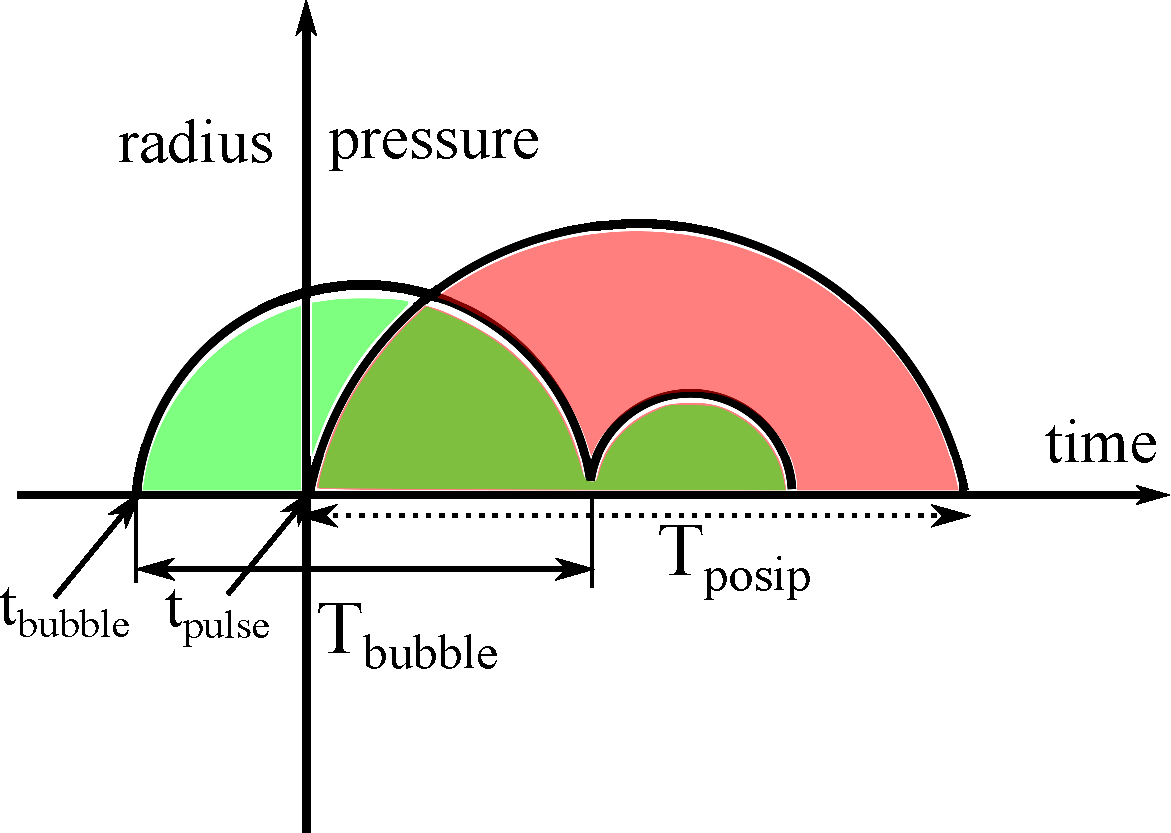
\includegraphics[width=0.5\linewidth]{img/fig5.1-eps-converted-to.pdf}
  \caption{空泡时间和压力波时间对比图。}
  \label{fig:5.1}
\end{figure}



在这里,我们关注空泡产生与压力波入射时间的时间差
$\Delta T =t_{\text{bubini}}-t_{\text{pulse}}$

我们定义一个无量纲变量,
$$\Delta \tilde{T} =\frac{t_{\text{bubini}}-t_{\text{pulse}}}{T_{\text{bubble}}}$$
此处, $t_{\text{bubble}}$
指空泡的出生时间,即激光击穿时间。$t_{\text{pulse}}$
指压力波前到达空泡位置的时间。而这两者的差即
$t_{\text{bubble}}-t_{\text{pulse}}$
为正时,压力波已经开始影响空泡位置,空泡产生在压力波的影响中。差为负时,指空泡产生并运动了一段时间后,压力波前到达空泡位置,并开始影响空泡脉动。
$T_{\text{bubble}}$指空泡的第一运动周期。这里通过这个空泡运动周期来规范化空泡诞生和压力波前到达空泡位置的时间差,这样$\Delta \tilde{T}$
表达了这个时间差与空泡第一脉动周期的相对尺度。$\Delta \tilde{T}<-1$时,压力波在空泡第一脉动周期结束后到达空泡。$-1<\Delta \tilde{T}<0$时,压力波在空泡第一脉动周期到达空泡,其中$-1<\Delta \tilde{T}<-0.6$压力波波影响空泡的溃灭过程,$-0.6<\Delta \tilde{T}<0.4$,压力波影响空泡的稳定阶段。$-0.4<\Delta \tilde{T}<0$压力波影响冲击波的膨胀阶段。$\Delta \tilde{T}>0$时,空泡诞生在压力波影响范围内。

同时,还存在一个压力波时间尺度与空泡生存时间的对比,即
$$\eta=\frac {T_\mathrm{bubble}}{T_\mathrm{posip}}$$ 其中
$T_\mathrm{posip}$
指压力波的正压时间跨度。如果压力波和击穿激光同时扰动空泡位置情景下,即
$\Delta T=0$,当 $\eta>1$ 时,空泡脉动会同时遭受正压和负压,
$\eta<1$ 时,空泡只在正压范围内运动。

本章分为两部分,分别从实验、和求解 K-M 方程的理论结果。


\section{撞击驱动的空泡运动}

如前文所述,撞击作为一种简单的冲击波产生方式有其独特的优势。本节采用第二章中介绍的试管撞击法产生冲击波。产生的高强度压力波沿着试管方向传播,经由界面反射回水体后形成舒张波。在这个压力波在水体中传播过程的不同阶段注入空泡,能够获得不同动力学反应。并运用高速摄影法获得其脉动机制。

\subsection{撞击压力波与激光空泡相互作用的高速摄像系统实现}

为了研究激光致空泡在自由落体和压力波作用下的复杂环境内的脉动,设计的实验安排如图\ref{fig:5.2} 所示。内径 13.5mm 的试管装了 150mm
深的除气去离子水,并在试管轴处击穿形成空泡。由于试管的圆柱形状不利于光学观察和激光聚焦,采用高透玻璃做透光面的棱柱形外围容器包裹,并充满水,以实现光学折射率匹配。这个容器放在一个导引轨道中,以使试管撞击底部铝镁合金平板于同一位置。一束
He-Ne 红光用来以光门方式触发光电二极管(DET10A2,
Thorlabs)和示波器。当试管通过并遮挡住光波路径,延迟发生器(BNC525,
Berkeley Nucleonics
Corporation)产生一系列外触发信号。而空泡通过激光脉冲(Q2, Quantum Light
Instruments, wavelength 532 nm, 6 ns
duration)聚焦到试管轴上产生。空泡动力学过程通过高速摄像机((Mini AX
200,
Photron)获得。另外一个光电二极管用来记录等离子体闪光。拍照视野通过散射匀光的
LED 灯(SugarCUBE, Edmund
Optics)照明。通过高速摄像机拍摄的系列图像,可以获得空泡的等效半径
$R(t)$,即计算截面气相面积,并推导同等面积情况下的圆半径,以之为空泡的半径
$R(t)$。而为了通过图像获得空泡截面面积,首先平均阈值二值化,并以
$2*2$ 像素的正方形开运算并闭运算来移除噪音。

\begin{figure}[H]
  \centering
  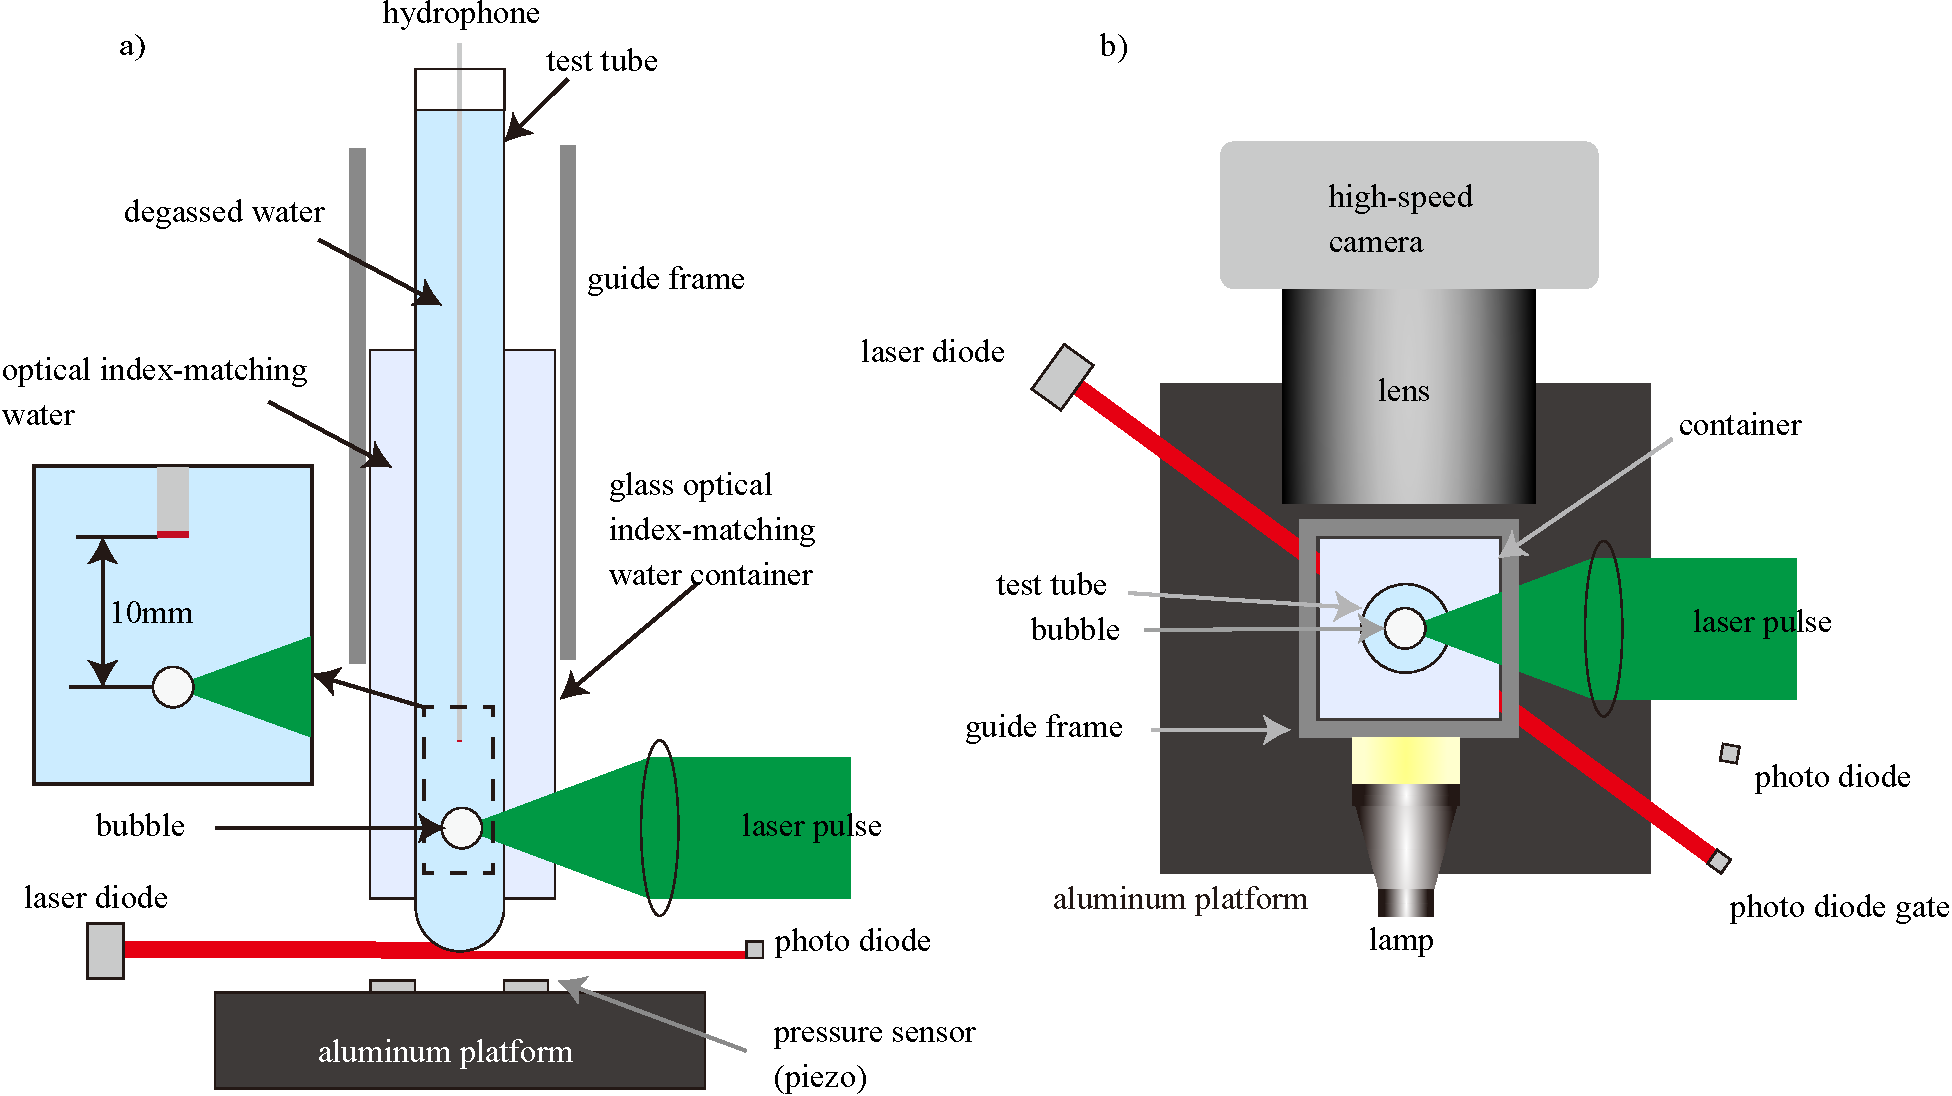
\includegraphics[width=0.8\linewidth]{img/fig5.2-eps-converted-to.pdf}
  \caption[本章的实验设置]{本章的实验设置。a)
是实验装置的侧视图,b)
是俯视图。激光、高速摄像机、和传感器连接并通过示波器和延迟发生器(BNC525)控制。试管在导引结构内下落,并逐渐阻挡光电二极管的光门。BNC525
由此产生触发信号到激光器和摄像机。随后光学击穿产生空泡。空泡的产生时间通过另外的光电二极管受等离子体闪光触发所获得。试管撞击到平台,并随后产生向试管内传播的压力波。摄像机记录整个过程(帧率
160000fps,曝光时间 1/900000 s,视野 $128*128\text{pixels}^2$)。}
  \label{fig:5.2}
\end{figure}

试管在距离金属板 50mm
处释放,并在本作中所有涉及到的撞击实验中保持这个固定距离。如此,如图 \ref{fig:5.3}
所示在试管撞击到平台后,一个压力脉冲产生并在试管内通过水体向上传播。其在声学软表面------液气界面发生反射,由此产生的舒张波向下回传到空泡产生位置。

\begin{figure}[H]
  \centering
  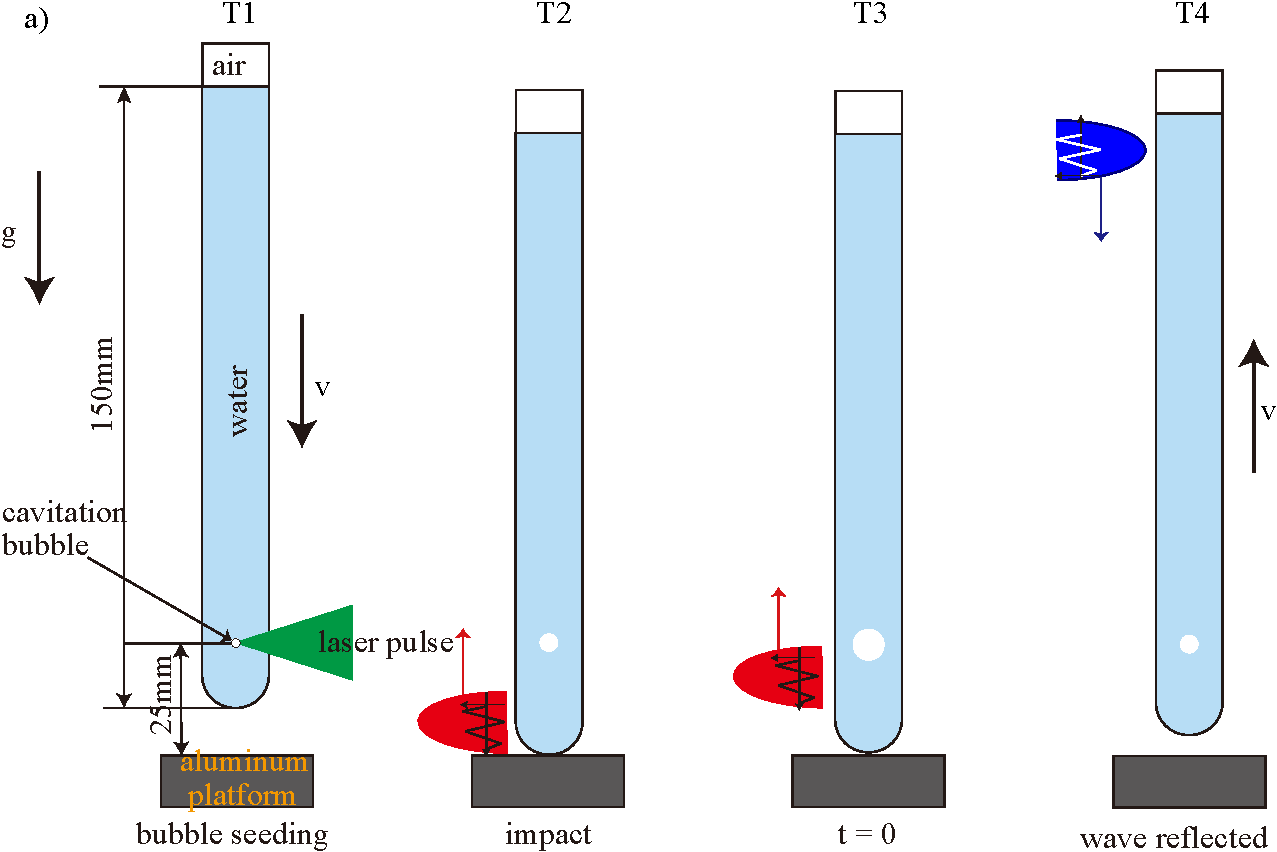
\includegraphics[width=0.6\linewidth]{img/fig5.3-eps-converted-to.pdf}
  \caption[压力波在试管内产生和传播的时序图]{压力波在试管内产生和传播的时序图。T1 到 T4
表示时间时间顺序。试管在撞击平台 (T2) 前自由降落
(T1)。撞击产生了一个压力波向上传播 (T3),并经过激光聚焦 (T1)
产生空泡的位置。经过水气界面反射后,压力波反射会水体内行成张力波 (T4)。
t =0 表示压力波波前第一次到达击穿位置的时刻。激光在 $t=-\Delta T$
时聚焦到距离平台 25mm 处。在研究关注的时间范围内,空泡不发生较大位移。}
  \label{fig:5.3}
\end{figure}


压力波波前经过空泡位置时刻与激光致空泡产生的时刻的时间差 $\Delta T$
可以控制在较大的范围内变化。为了精准的获得撞击时间,将一个压电陶瓷压力传感器(SMD05T04R411,
STEMINC)粘贴到金属平台靠近撞击点的位置。并将一个针状水听器(Müller-Platte)布置到空泡产生位置。通过无激光入射情况下,同高度释放撞击,并记录压电陶瓷的脉冲时间与水听器的脉冲时间差,可以获得撞击后金属板上的弹性波脉冲波前到达压力传感器与水中压力波前到达水听器位置也就是后续空泡产生位置的时间差。在后续数据处理中,利用这个时间差以及压电陶瓷获得的压力信号,推算压力波波前到达空泡位置的时间。值得注意的是,水听器的接口不影响试管的自由落体,重复性的加载水听器或者卸载水听器的实验获得相似的结果。一个典型的水听器波形记录如图
\ref{fig:5.4} 所示。

\begin{figure}[H]
  \centering
  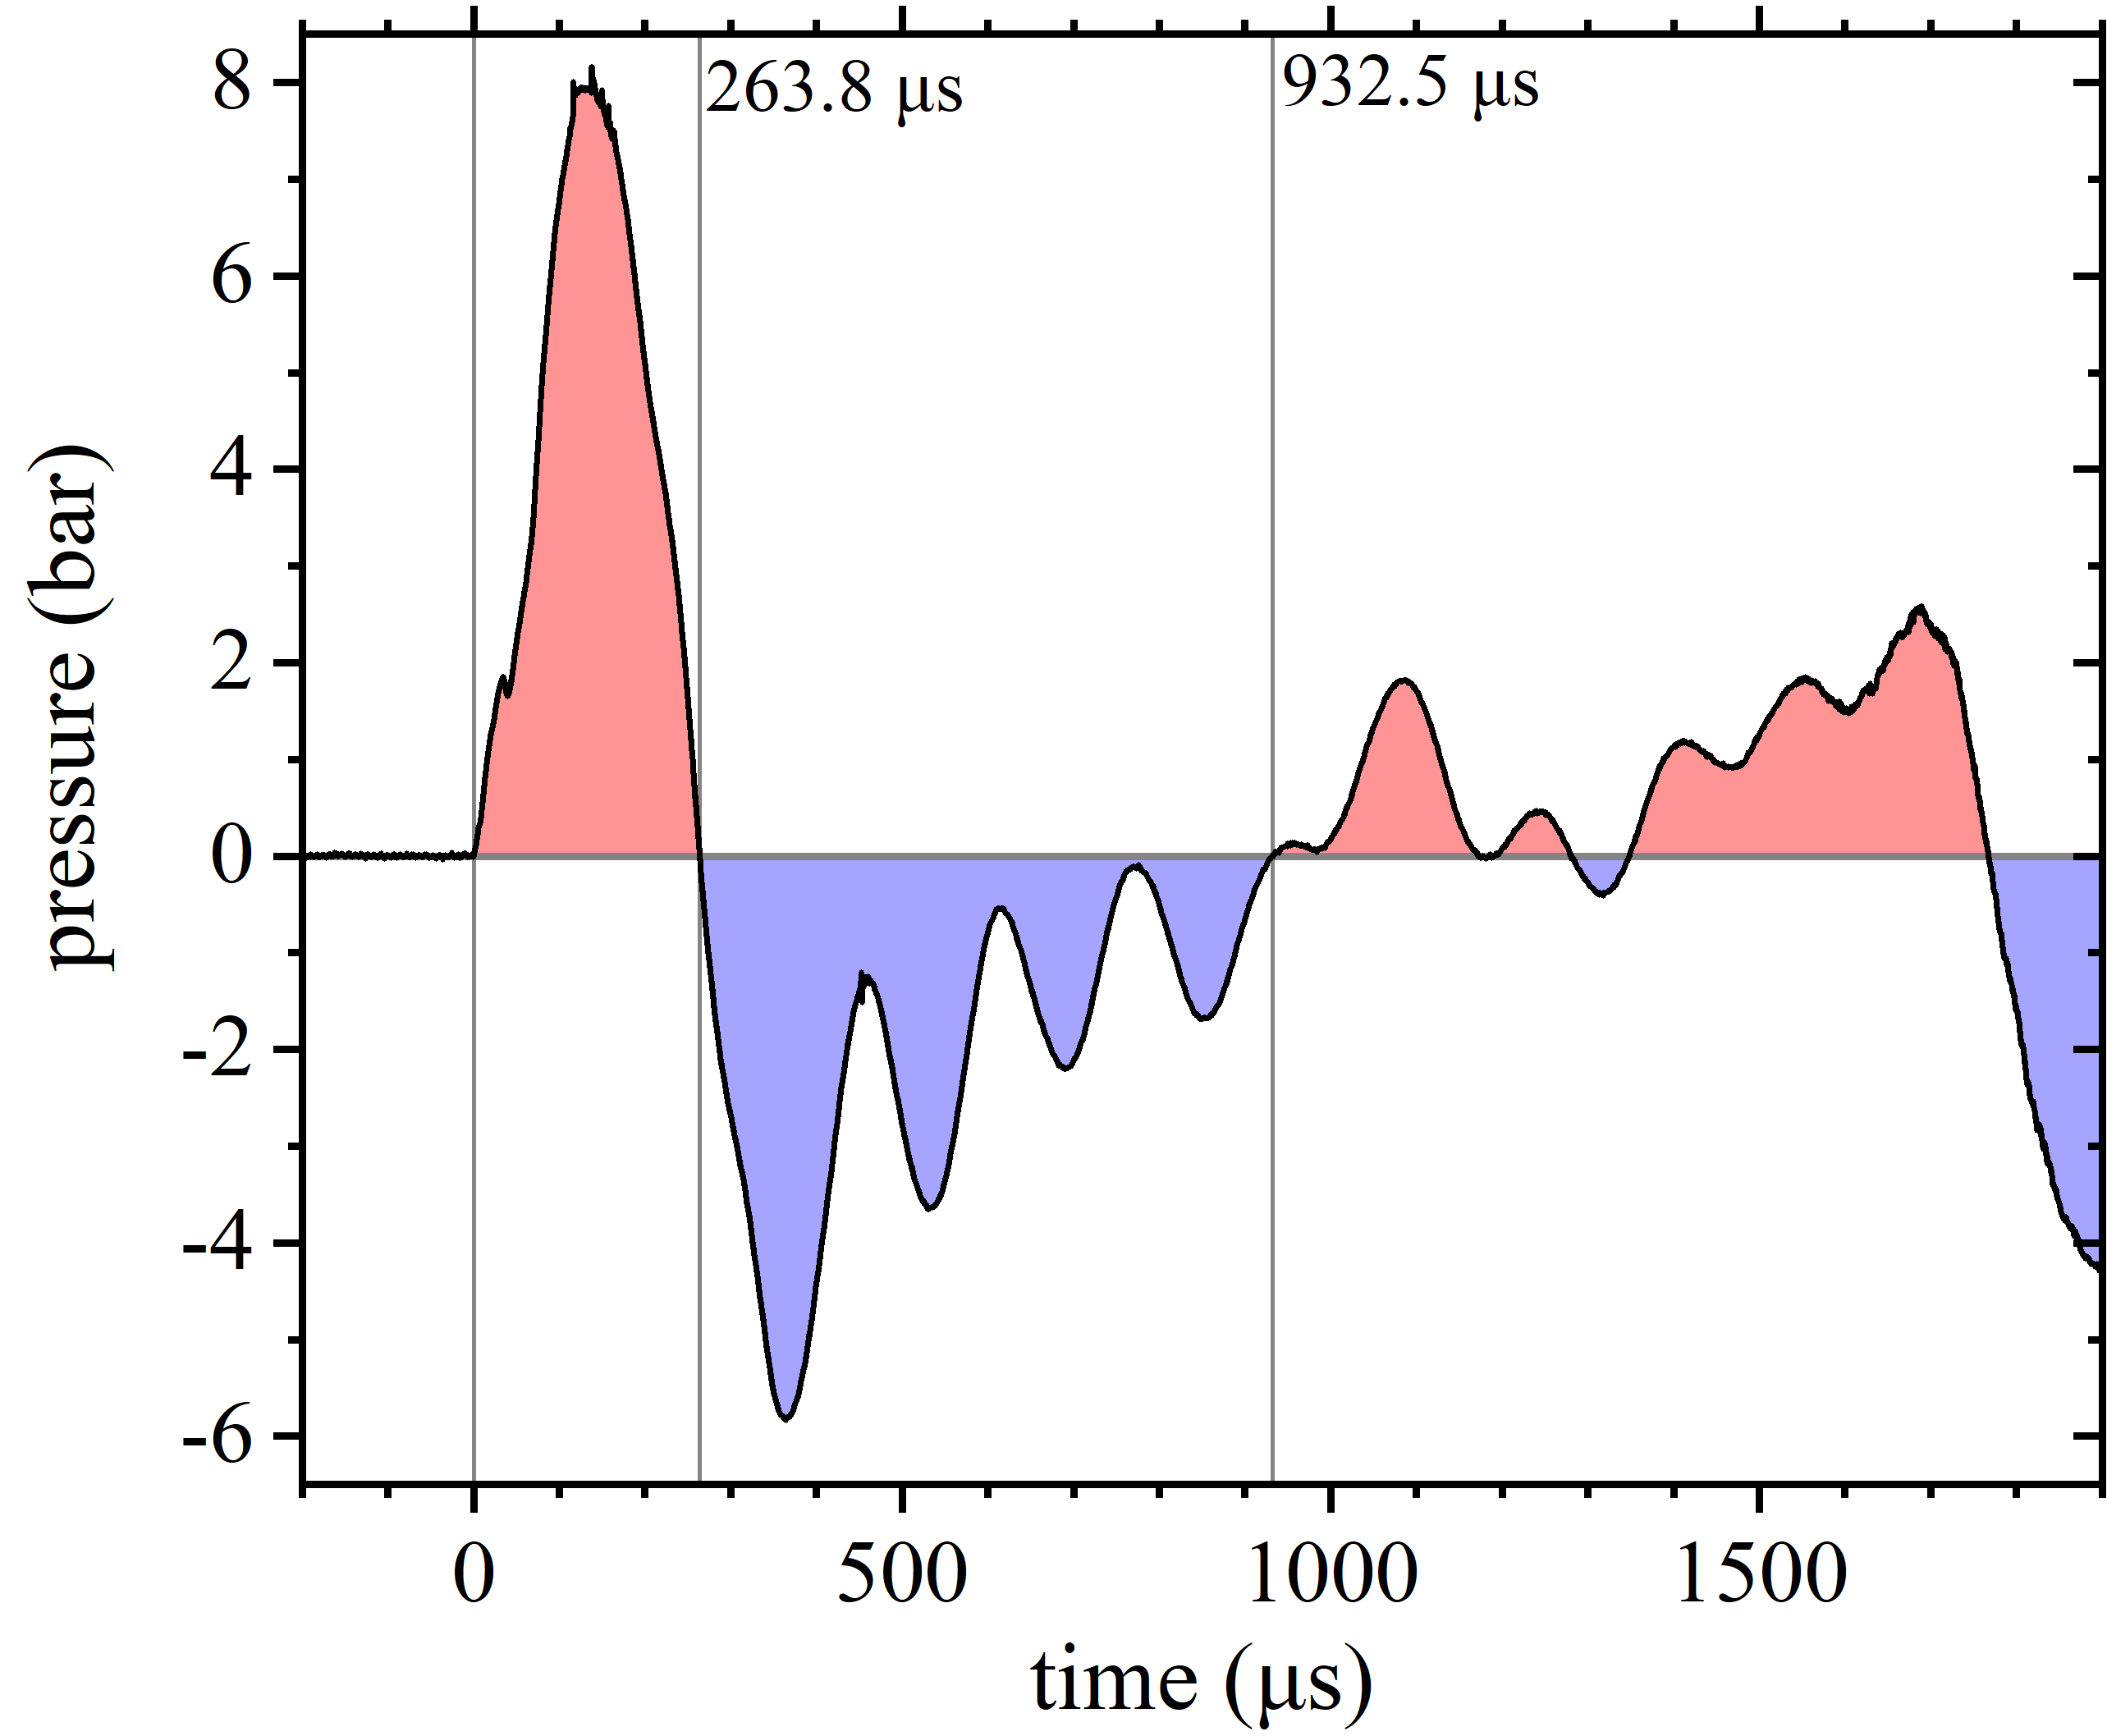
\includegraphics[width=0.6\linewidth]{img/fig5.4.png}
  \caption[冲击压力波,$p_i$,在未射入激光情况下原击穿位置测得(十次平均)]{冲击压力波,$p_i$,在未射入激光情况下原击穿位置测得(十次平均)。压缩相用红色标识,舒张相(反射导致)用蓝色标识。}
  \label{fig:5.4}
\end{figure}

从波形中可以看到,撞击后产生的压力波,传播到空泡位置的压力最高可以 8bar
左右。由于撞击压力的衰减和自由水气界面的反射形成的张力波作用,在 150
$\mu$ s 左右开始下降,并在 263.8 $\mu$ s
处下降到静压以下。压力舒张一直持续到 932.5 $\mu$ s。
除了撞击外,激光击穿同时也产生一个瞬态的压力脉冲。为了区分并考虑这两个压力源,分别记录了在无激光情况下撞击和无撞击情况下的激光击穿的压力波形。图\ref{fig:5.5}
显示了只有激光击穿压力情况的水听器压力记录。此时试管静止的放在平台上,而水听器放在击穿点正上方2mm处。该波形记录了空泡击穿冲击波信号,该击穿冲击波的反射波,以及空泡溃灭冲击波。从图中的击穿冲击波到溃灭冲击波的时间间隔测得的空泡生存时间约97 $\mu$ s。冲击波在 2mm范围内的速度较本地声速快,但这里将其处理成声速,形成的时间误差远小于空泡生存时间,故而忽略这个差别。

\begin{figure}[H]
  \centering
  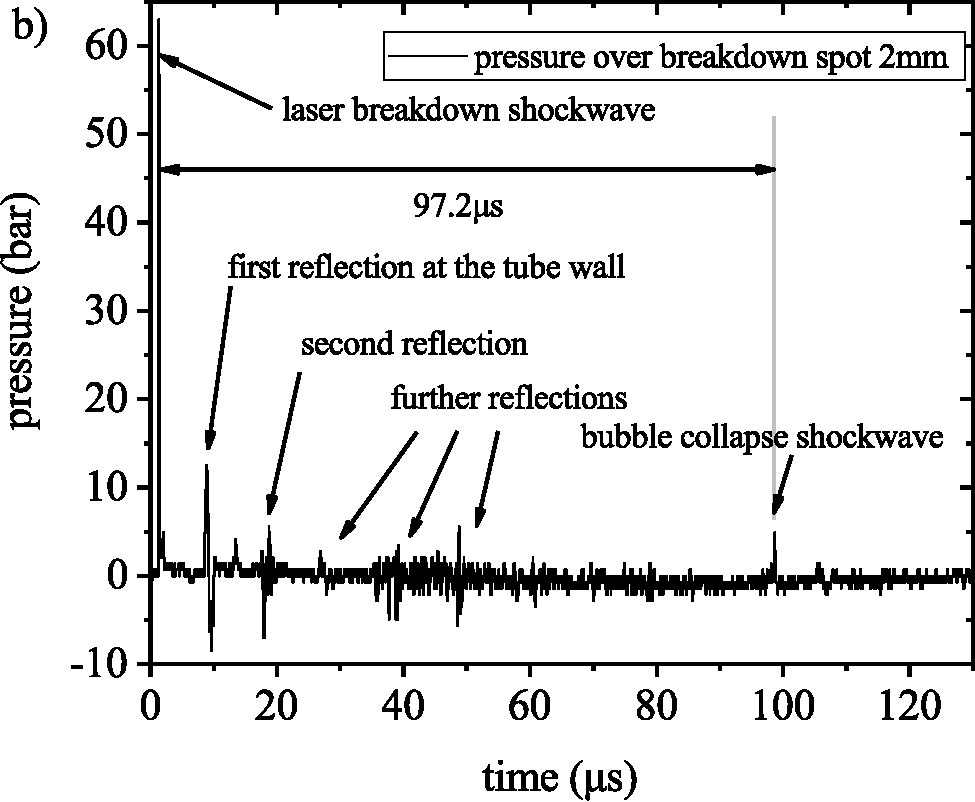
\includegraphics[width=0.8\linewidth]{img/fig5.5-eps-converted-to.pdf}
  \caption[激光击穿冲击波压力]{激光击穿冲击波压力,在无冲击情况下的静态试管中,激光击穿位置上方 2mm
处测得的压力。}
  \label{fig:5.5}
\end{figure}

撞击产生的压力波与图 \ref{fig:5.5}
中显示的反射冲击波将在后续中结合,以重建空泡位置的压力。这是因为以现在的条件水听器不能直接放置在激光击穿位置并获得空泡遭受的压力,并且越靠近击穿位置,空泡将与水听器发生更加强烈的相互作用。如此,为了将实验与
Keller-Miksis 模型相比较,我们需要对空泡位置压力做一个更好的物理预估。
在降落和撞击实验中,空泡在其位置上遭受的压力 $p(t)$
可以看成两个压力的叠加,撞击产生的压力波 $p_i$
和激光击穿冲击波的反射波 $p_s$,即
$p (t)= p_i(t)+ p_s(t)$。通过有限元法(COMSOL
Multiphysics)模拟计算获得,空泡位置处收到的压力与 2mm
处压力相差不超过一个数量级。通过与实验结果的拟合(最小方差法),获得最佳重建压力比例系数为
k=8.3。即,可以将 2mm 处测得的反射波压力乘以
k,并添加时延后获得重建的空泡所受的压力,$p_s (t)=k p_\mathrm{hyd}^\mathrm{2mm}(t+\Delta t)$
。后续针对实验的数值计算中,使用这个压力当作空泡的驱动声压。

\begin{figure}[H]
  \centering
  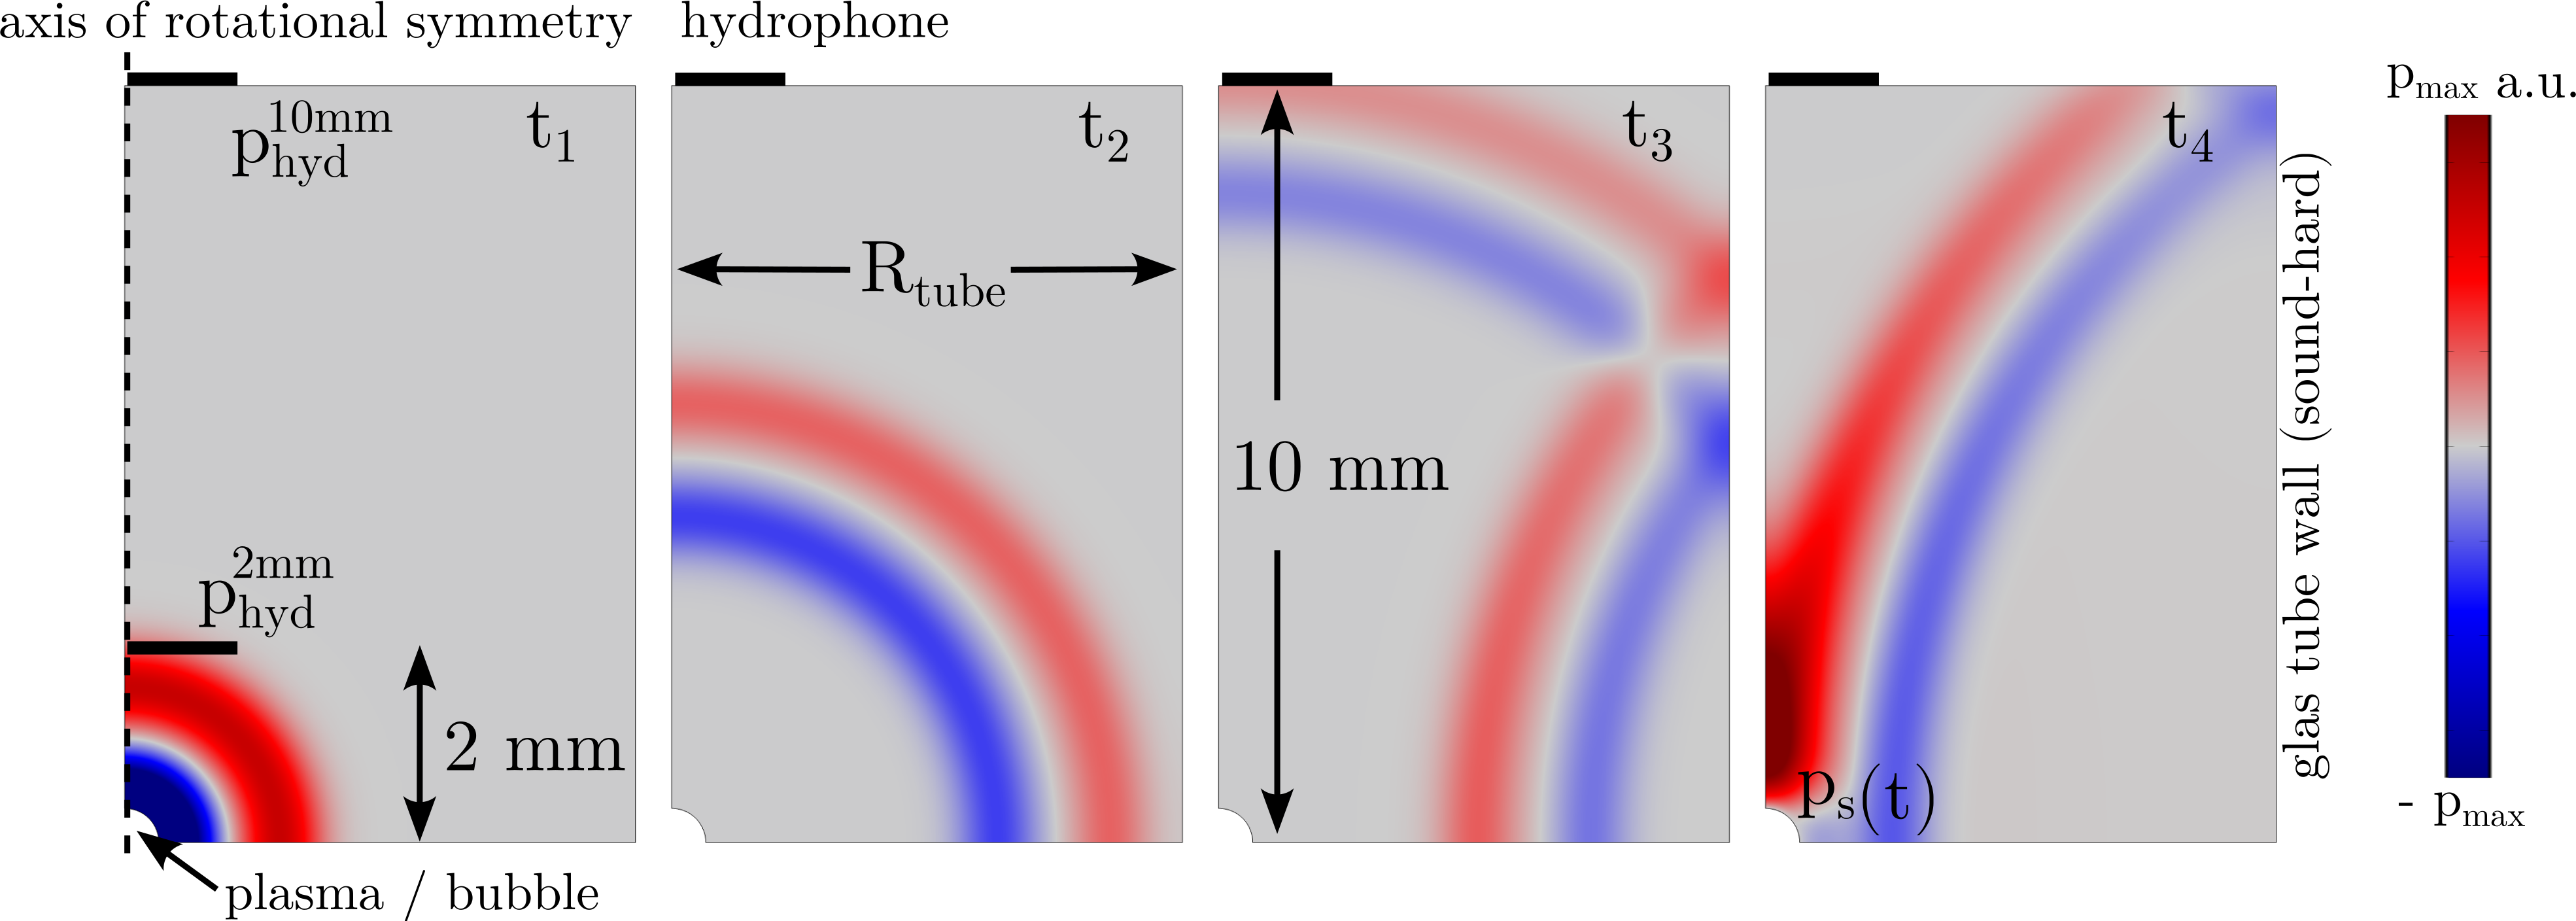
\includegraphics[width=1\linewidth]{img/fig5.6.png}
  \caption{comsol
模拟获得压力重建乘数 k。}
  \label{fig:5.6}
\end{figure}

\begin{figure}[H]
  \centering
  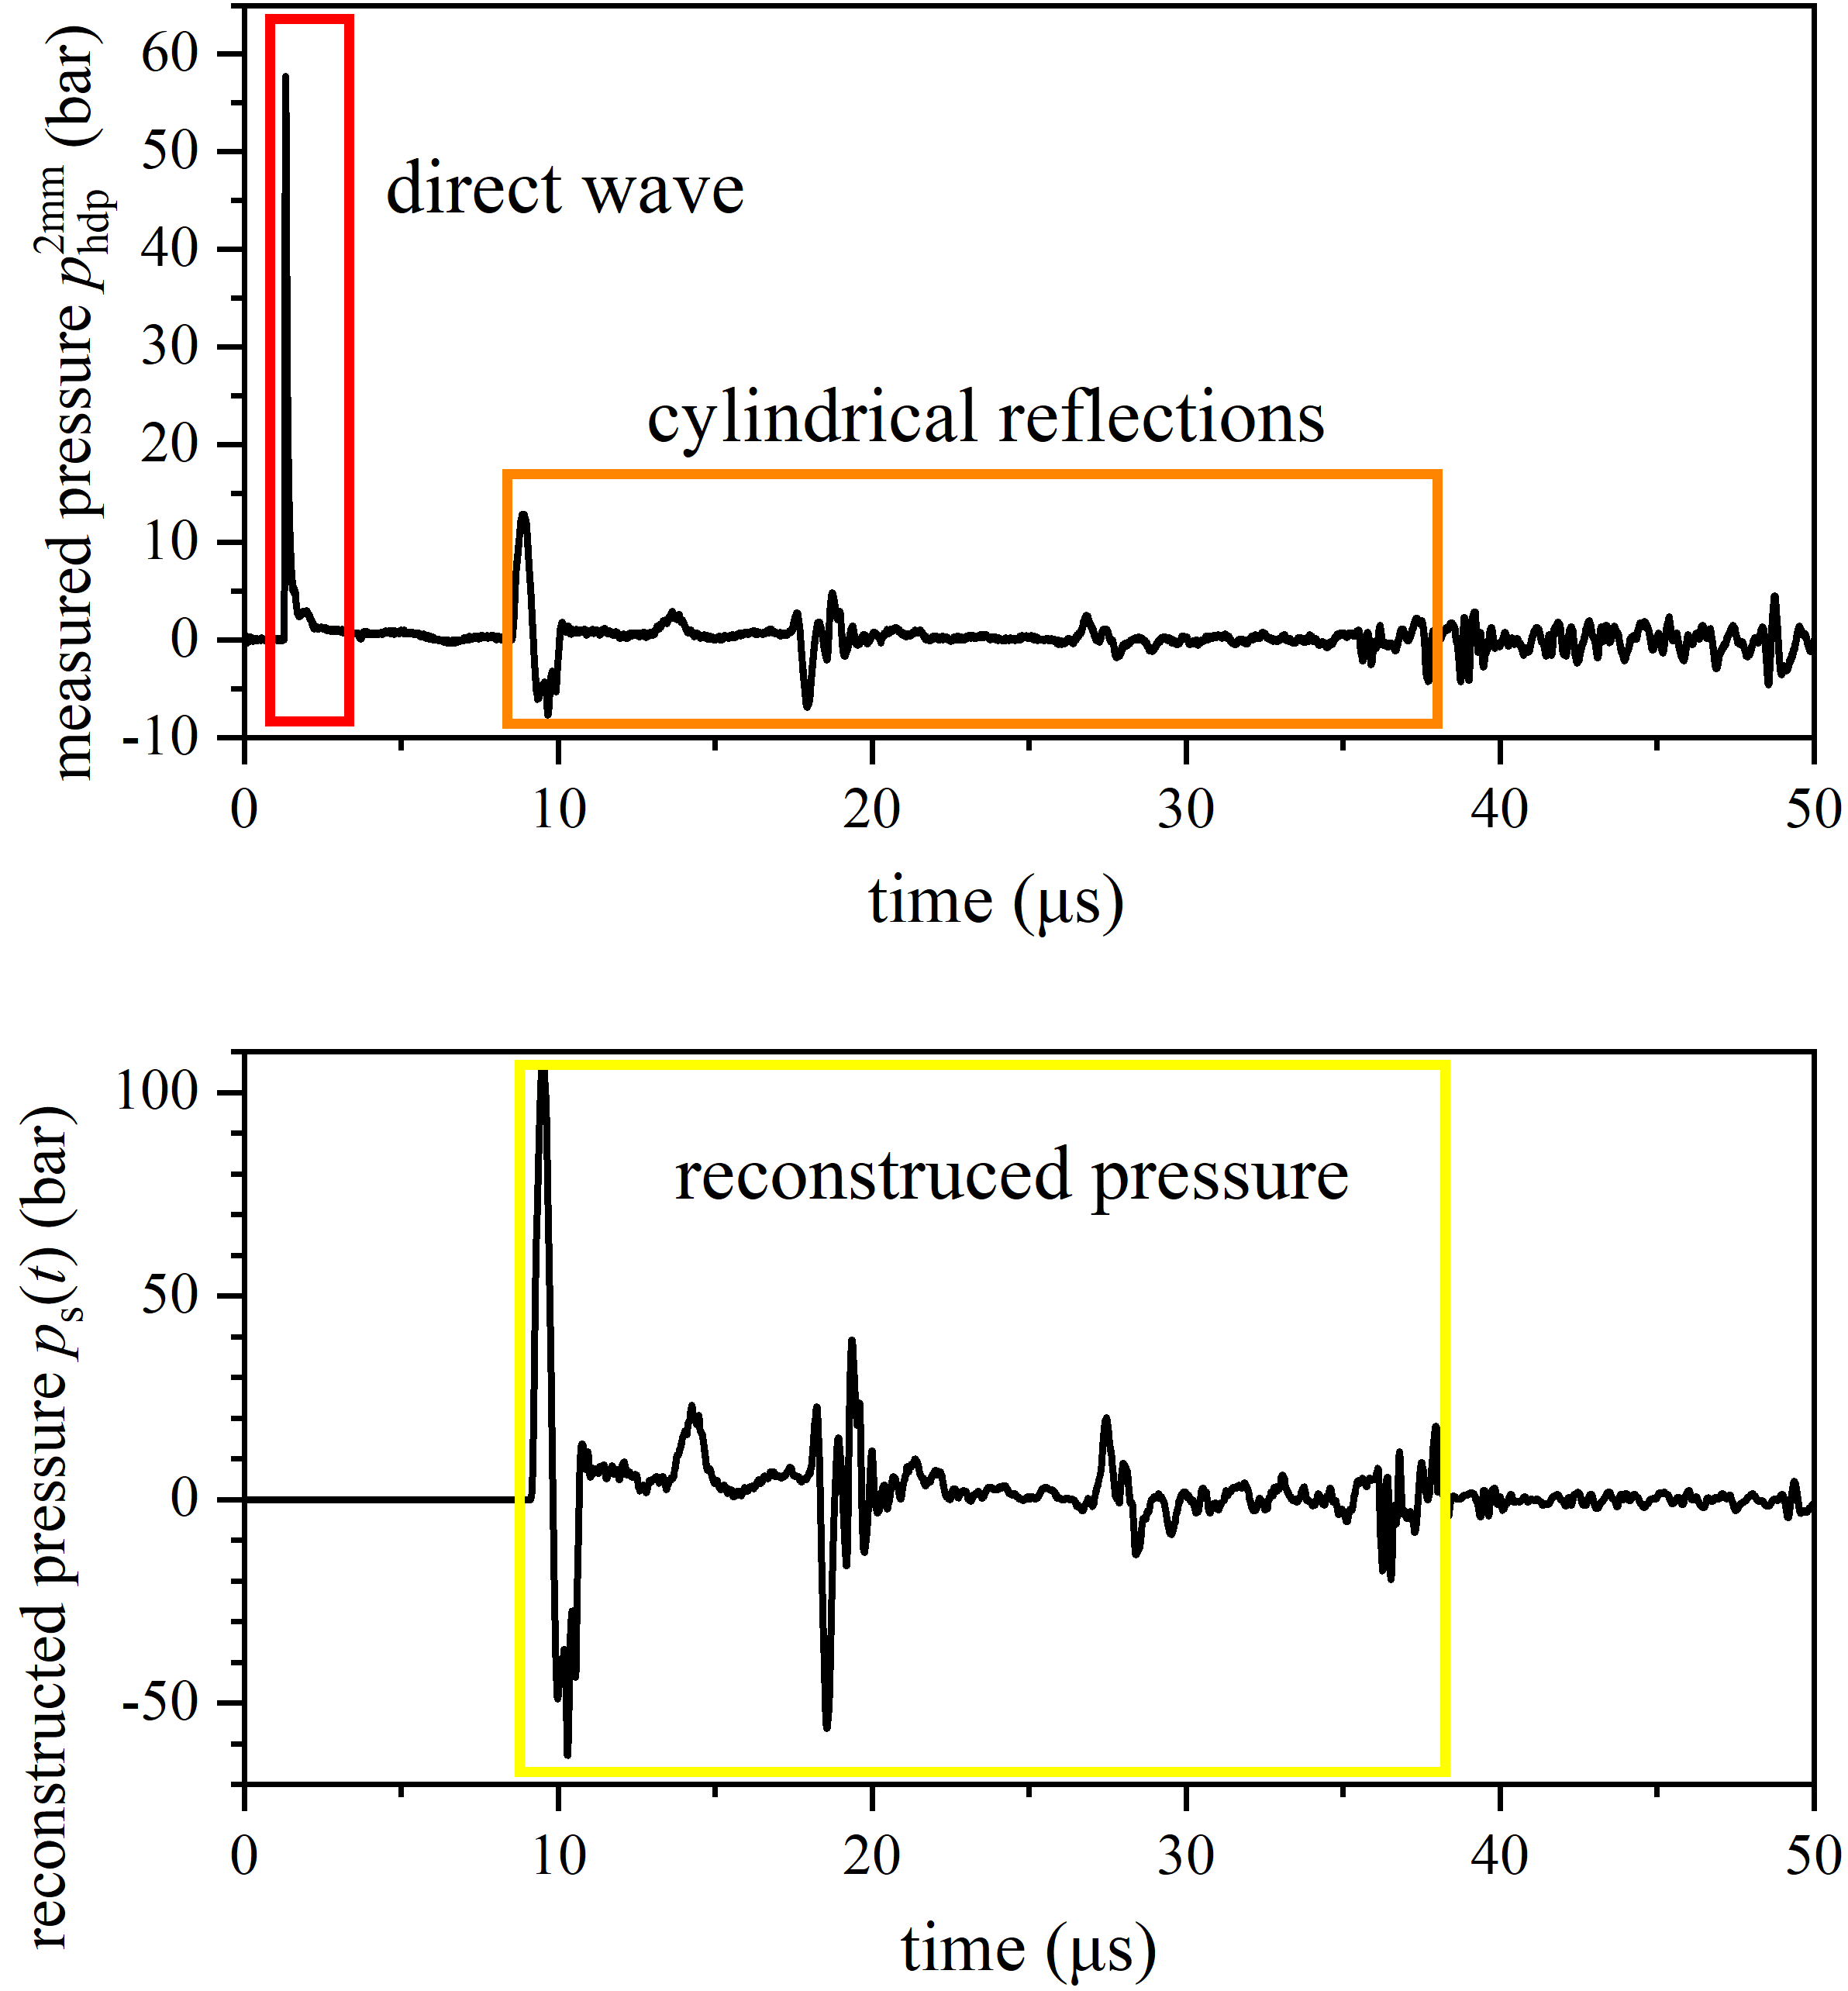
\includegraphics[width=0.6\linewidth]{img/fig5.7.png}
  \caption[利用 2mm
处测得的压力(上)重建空泡处(下)压力]{利用 2mm
处测得的压力(上)重建空泡处(下)压力。重建压力在反射波到达前设置为
0。在受到影响后为
$p_s (t)=k p_\mathrm{hyd}^\mathrm{2mm}(t+\Delta t)$。并截至到 38
$\mu$ s,其后使用测得压力,并在空泡溃灭冲击波处后再次设置为 0。}
  \label{fig:5.7}
\end{figure}

\begin{figure}[H]
  \centering
  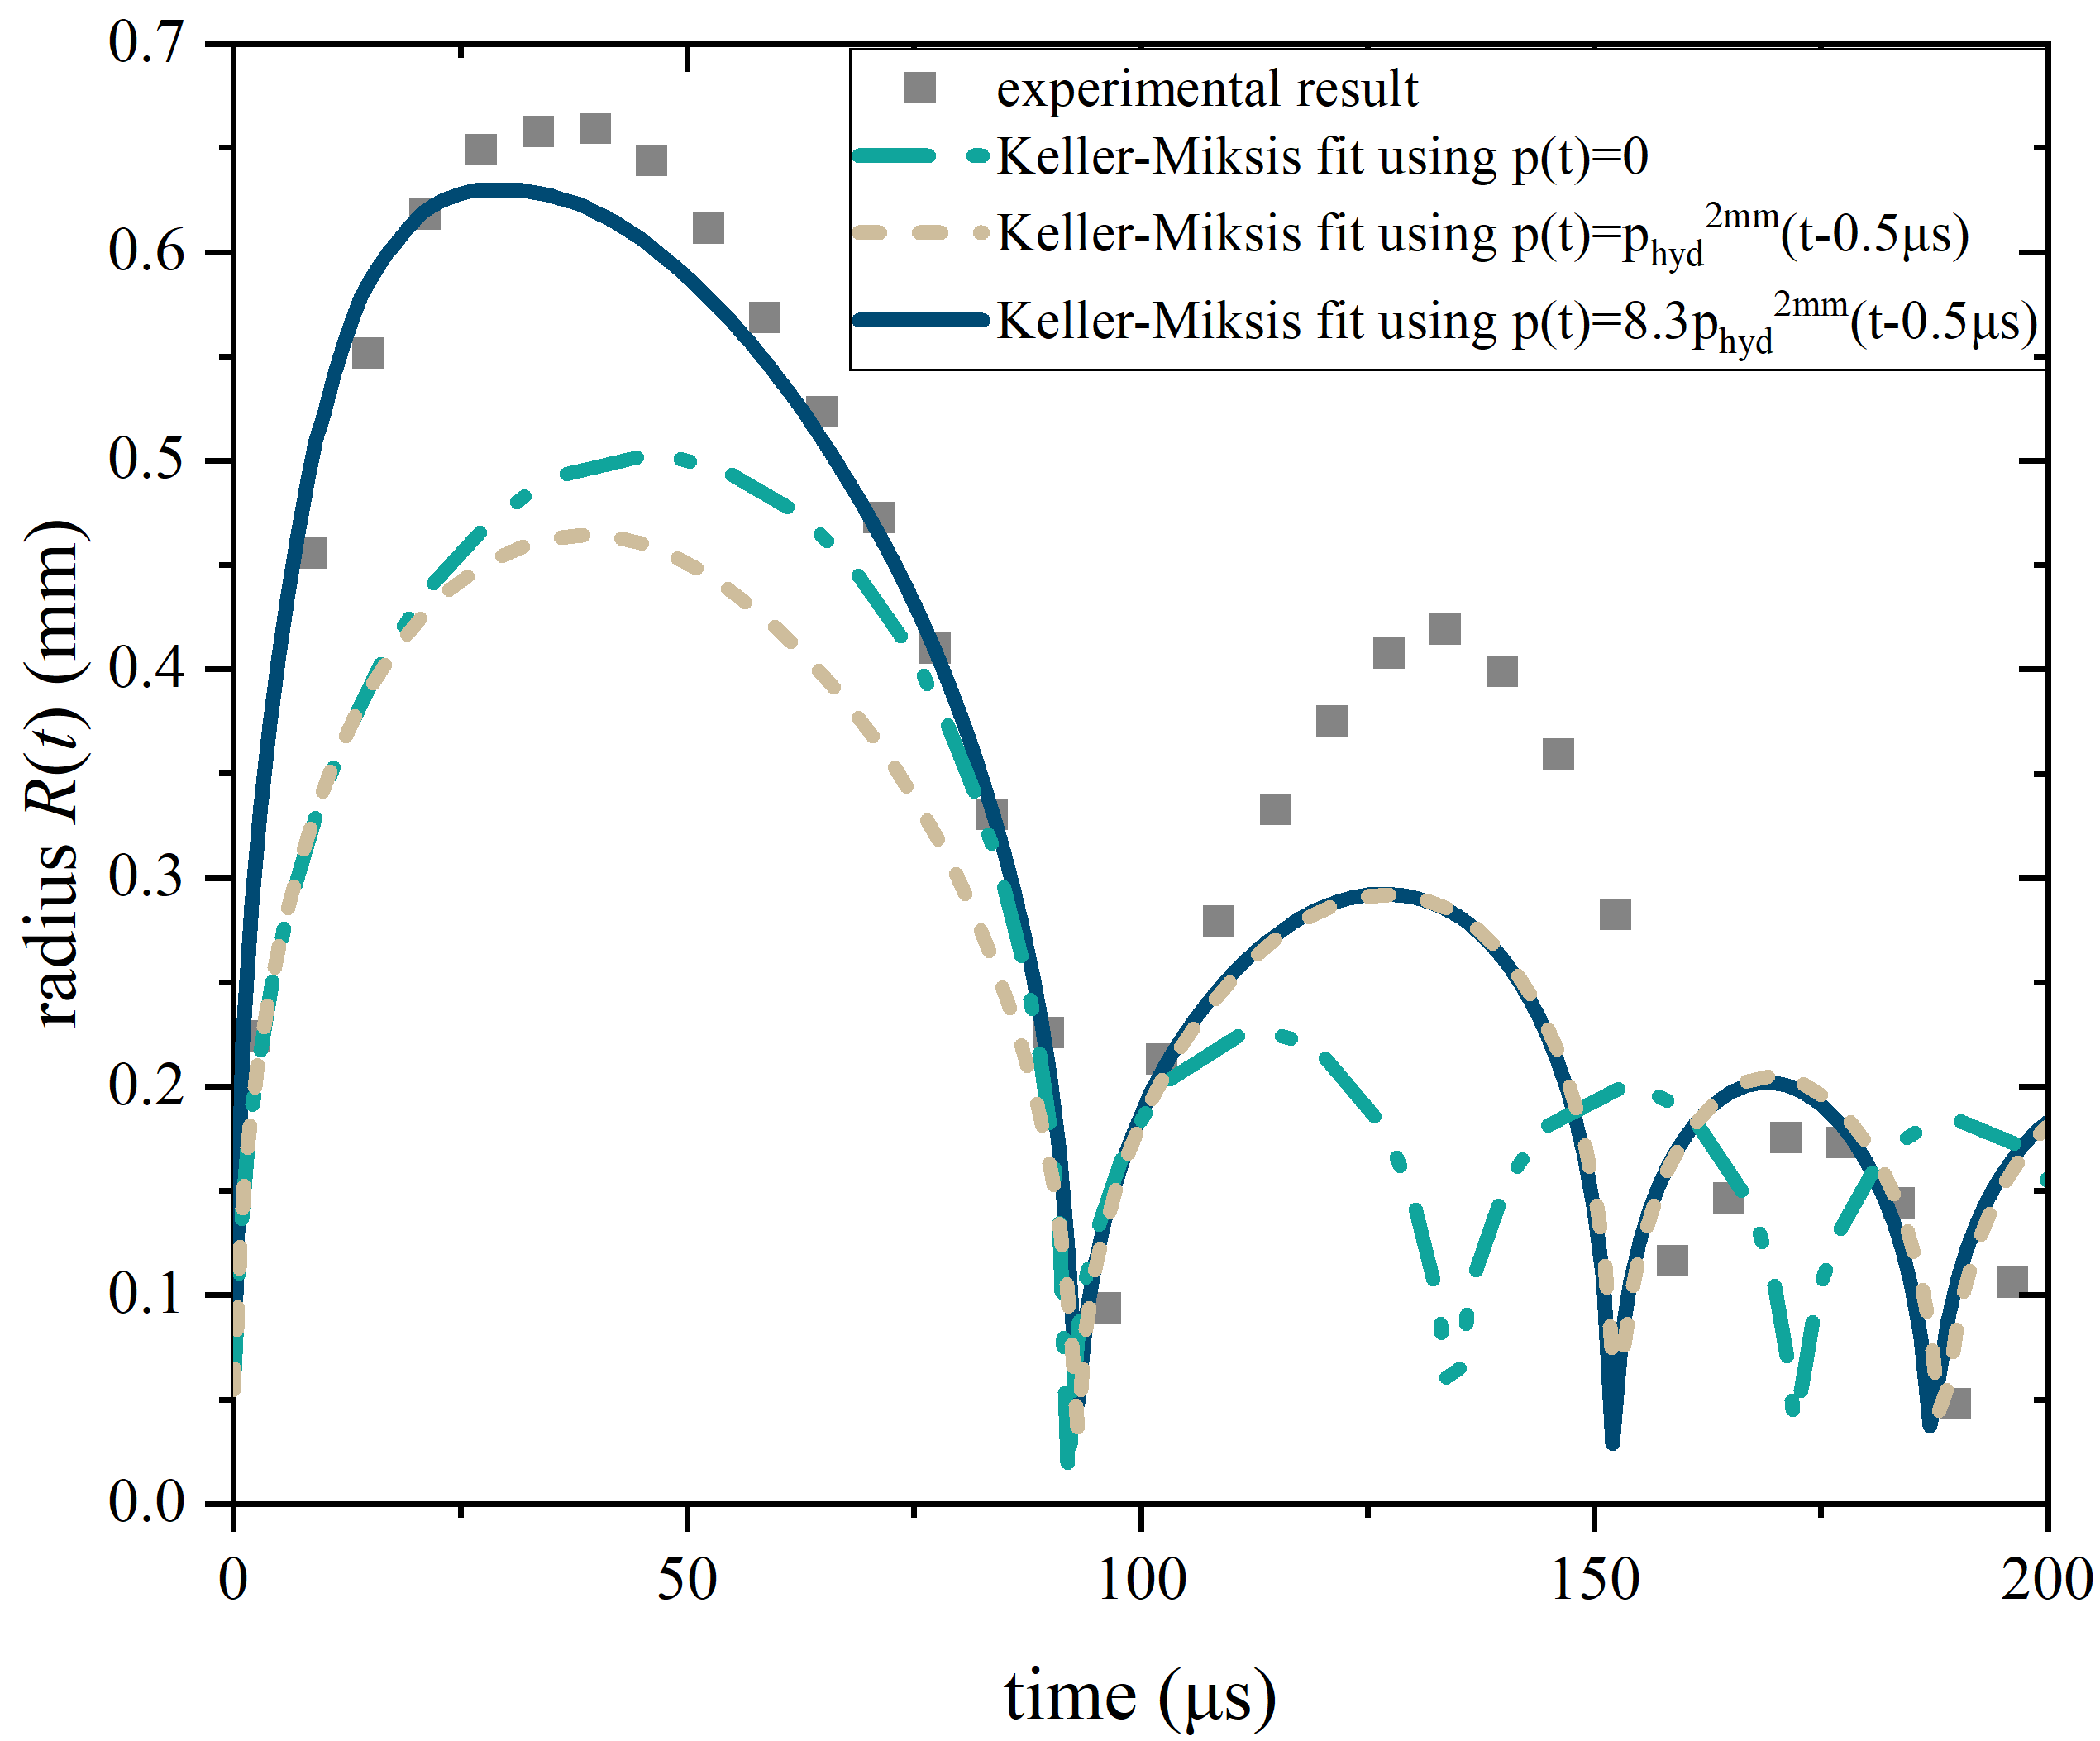
\includegraphics[width=0.7\linewidth]{img/fig5.8.png}
  \caption[利用重建的压力代入
Keller-Miksis
模型计算获得的空泡半径与使用其他压力的对比]{利用重建的压力代入
Keller-Miksis
模型计算获得的空泡半径与使用其他压力的对比。实验半径采自静止试管实验。模型计算的初值为
$R (t = 0) = 54.5\,\mathrm{mm}$,重建压力案例的初始速度为 1280
m/s,直接使用 2mm 水听器压力的案例初始速度为 540
m/s,使用静压条件的案例初始速度为 260m/s。所有案例在 94 $\mu$ s
左右处溃灭。均衡半径取自静止实验中 1ms 时,残余气体形成的小空泡
$R_0=0.09$mm。}
  \label{fig:5.8}
\end{figure}
在后续实验中,水听器放置在击穿点上方 10mm,以检测系列实验中的压力。


\subsection{静止和自由落体中空泡脉动的对比}

在特定高度释放试管后,试管内液体在试管撞击金属板处于失重状态。此时击穿水体形成空泡,空泡处于一个零加速度场中。

图\ref{fig:5.9}
上行显示了激光产生的空泡在无干预情况下,也就是试管静止时的动力学过程。它在本章中作为一个与自由落体和撞击情况的参照存在。在所有实验中,
$t=0$ 是激光击穿形成闪光的时刻,此时当作空泡的开始。在空泡形成后,其在
$t \approx 39.9\,\mu s$ 时能达到最大泡半径约为
$R_\textrm{max}=0.69\,mm$,并在 $t=96.1\,\mu \mathrm{s}$
时溃灭。因为试管体积的限制,这使得空泡的膨胀相和收缩相不再对称,这与在准自由场(即空泡距离边界
$20*R_{\text{max}}$
以上)中产生的空泡存在差别。这种现象可以用激光击穿冲击波及其后续反射波对膨胀相空泡的影响来解释。当空泡产生在立方体水箱中时,击穿冲击波因平面反射的缘故,不会在空泡位置产生汇聚效应,所以通常在水箱实验中忽略这种聚焦效应。但在此处实验中,因空泡产生在具有圆形界面的试管中央,击穿冲击波部分被试管玻璃壁面反射回空泡位置,从而影响空泡脉动。而冲击波产生到返回的时间大约是
$10\,\mu$
s,此时空泡处于膨胀相,使得空泡的膨胀现象受到明显抑制,具体推导见第二章实验设置。但相较于撞击产生的高强度,长持续时间的压力脉冲,这个聚焦冲击波对空泡的影响只有短时的压缩效果,对空泡整体上的膨胀和收缩过程的影响远远小于撞击冲击波。并不影响我们使用这种手段来研究撞击冲击波对空泡的作用机制。

在空泡溃灭后,空泡回弹,并在约 $t=139.9\,\mu \mathrm{s}$
时到达二次脉动的最大泡半径 $R_\textrm{max2}=0.43\,\mathrm{mm}$
,然后再次在 $t=164.9\,\mu \mathrm{s}$
时溃灭。这之后,空泡仍然持续脉动,直到泡能消耗。这个过程约持续到
$t=400\,\mu \mathrm{s}$ ,并因浮力作用而逐渐上浮,离开空泡原位置。图\ref{fig:5.9}
所示的两例空泡脉动半径曲线图在图 \ref{fig:5.12} 中显示为黑色和红色的点。

图\ref{fig:5.9} 
底行自由落体案例的空泡脉动的动力学过程。此自由落体案例是指,在特定高度释放试管后,射入激光产生空泡,空泡在试管撞击金属平面前的后续脉动过程。空泡在自由落体和静止状态下的动力学表现非常相似。
图 \ref{fig:5.10}
也显示两种不同帧率拍摄下获得的空泡半径随时间变化的曲线。cut-method
是将高速摄像取较小的分辨率($8*128$)以获得较高的帧率,而只拍摄到如切片一般的空泡中心区域阴影的方法。试管的微位移造成的空泡位置变动是
cut-method
测得空泡半径变化的主要因素。多次采样间的激光能量密度,和试管微位移造成的击穿冲击波及其后续压力波变化,是影响多次测量间不同结果的主要因素。
针对自由落体和静止状态案例,我们认为在空泡尺寸不够大的情况下,重力的影响十分微弱。在第三章中给出的参数$\zeta=-\rho g R_{\text {max}} \Delta p^{-1}$,可以间接的用来表达空泡形变的程度。在实验案例中,设定最大泡半径为
$R_\textrm{max}=0.7\,$mm,环境压强 $p_a=1\,$bar ,获得的
$\zeta= 7\,*10^{-5}$,远远小于能够产生微射流的阈值$\zeta = 10^{-3}$。这也证明在百微米和毫米尺寸的空泡完全可以忽略重力的作用。

\begin{figure}[H]
  \centering
  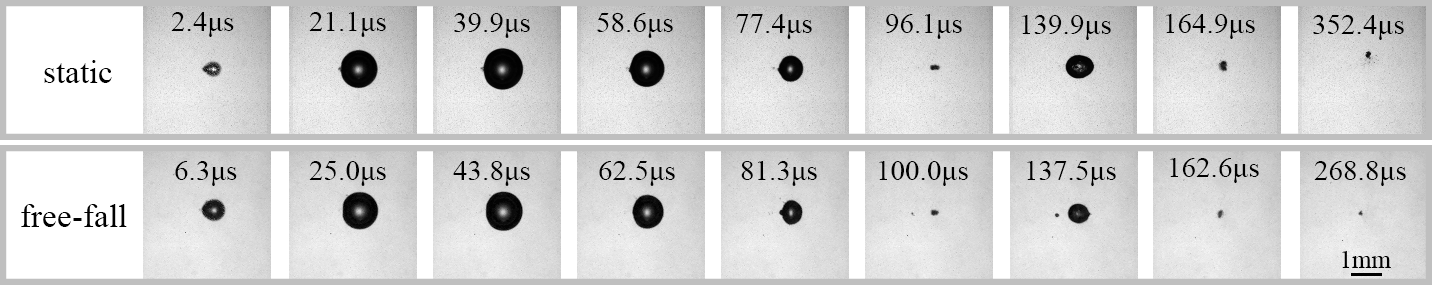
\includegraphics[width=1\linewidth]{img/fig5.9.png}
  \caption[静态和自由落体环境下的空泡动力学过程的照片]{静态和自由落体环境下的空泡动力学过程的照片。每一帧照片对应的时间标注在图片上方。上下栏分别对应了静态和自由落体的案例。标尺标注于于下栏的末端。激光自每帧图片的右方射入,而撞击产生的压力波垂直的自下而上传播。
}
  \label{fig:5.9}
\end{figure}




\begin{figure}[H]
  \centering
  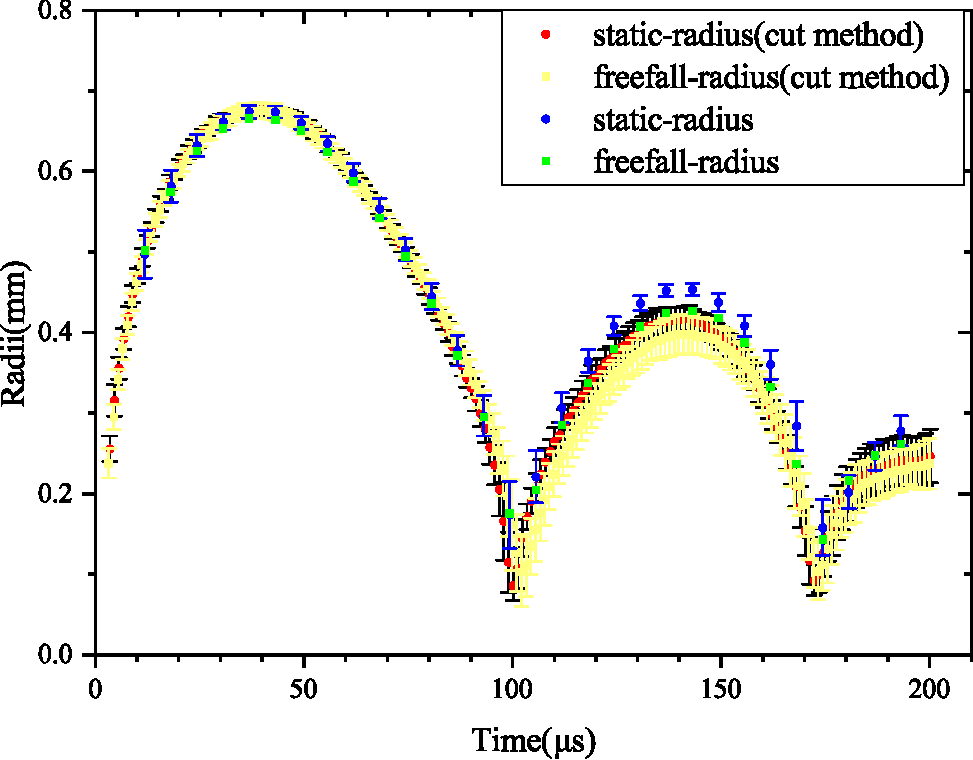
\includegraphics[width=0.7\linewidth]{img/fig5.10-eps-converted-to.pdf}
  \caption[两种方法测得的空泡半径对比]{将相机图像中心稳定到空泡初生位置,分别采用大帧率小视野(cut
method)、和大视野小帧率两种方法获得空泡的半径。前者使用最远距离为空泡直径,后者使用面积法获得半径。误差由十次采样的平均方差表示。
}
  \label{fig:5.10}
\end{figure}




\subsection{瞬态压强驱动的空泡及空泡团簇的运动}

图\ref{fig:5.11}
是显示了在不射入激光的情况下,试管自由下降并撞击金属平台,在空泡产生位置测量得的撞击压力波。正压力波持续了
$263\,\mu$ s,随后进入舒张波阶段。舒张波持续到 $t=932\,\mu$
s。并继之一些后续波动。在整个压力波阶段,正压可以达到 $8\,$
bar,而负压能达到 $-5.5\,bar$ 。

本节将讨论四种不同空泡产生时间相位下的空泡动力学。空泡的产生如图 \ref{fig:5.11}. b
所示。''L''代表激光入射时间。静态情况下,空泡的第一脉动周期持续
$96\,\mu$ s,小于在脉冲压力的正向周期。
四种情况分别是:(a)空泡先于压力脉冲产生;(b)空泡在脉冲正压的波峰附近产生;(c)空泡先于负压开始产生;(d)空泡在负压中产生。此四种情况在图\ref{fig:5.11}
中显示。对应的实验图的时序也标识在该图中。

\begin{figure}[H]
  \centering
  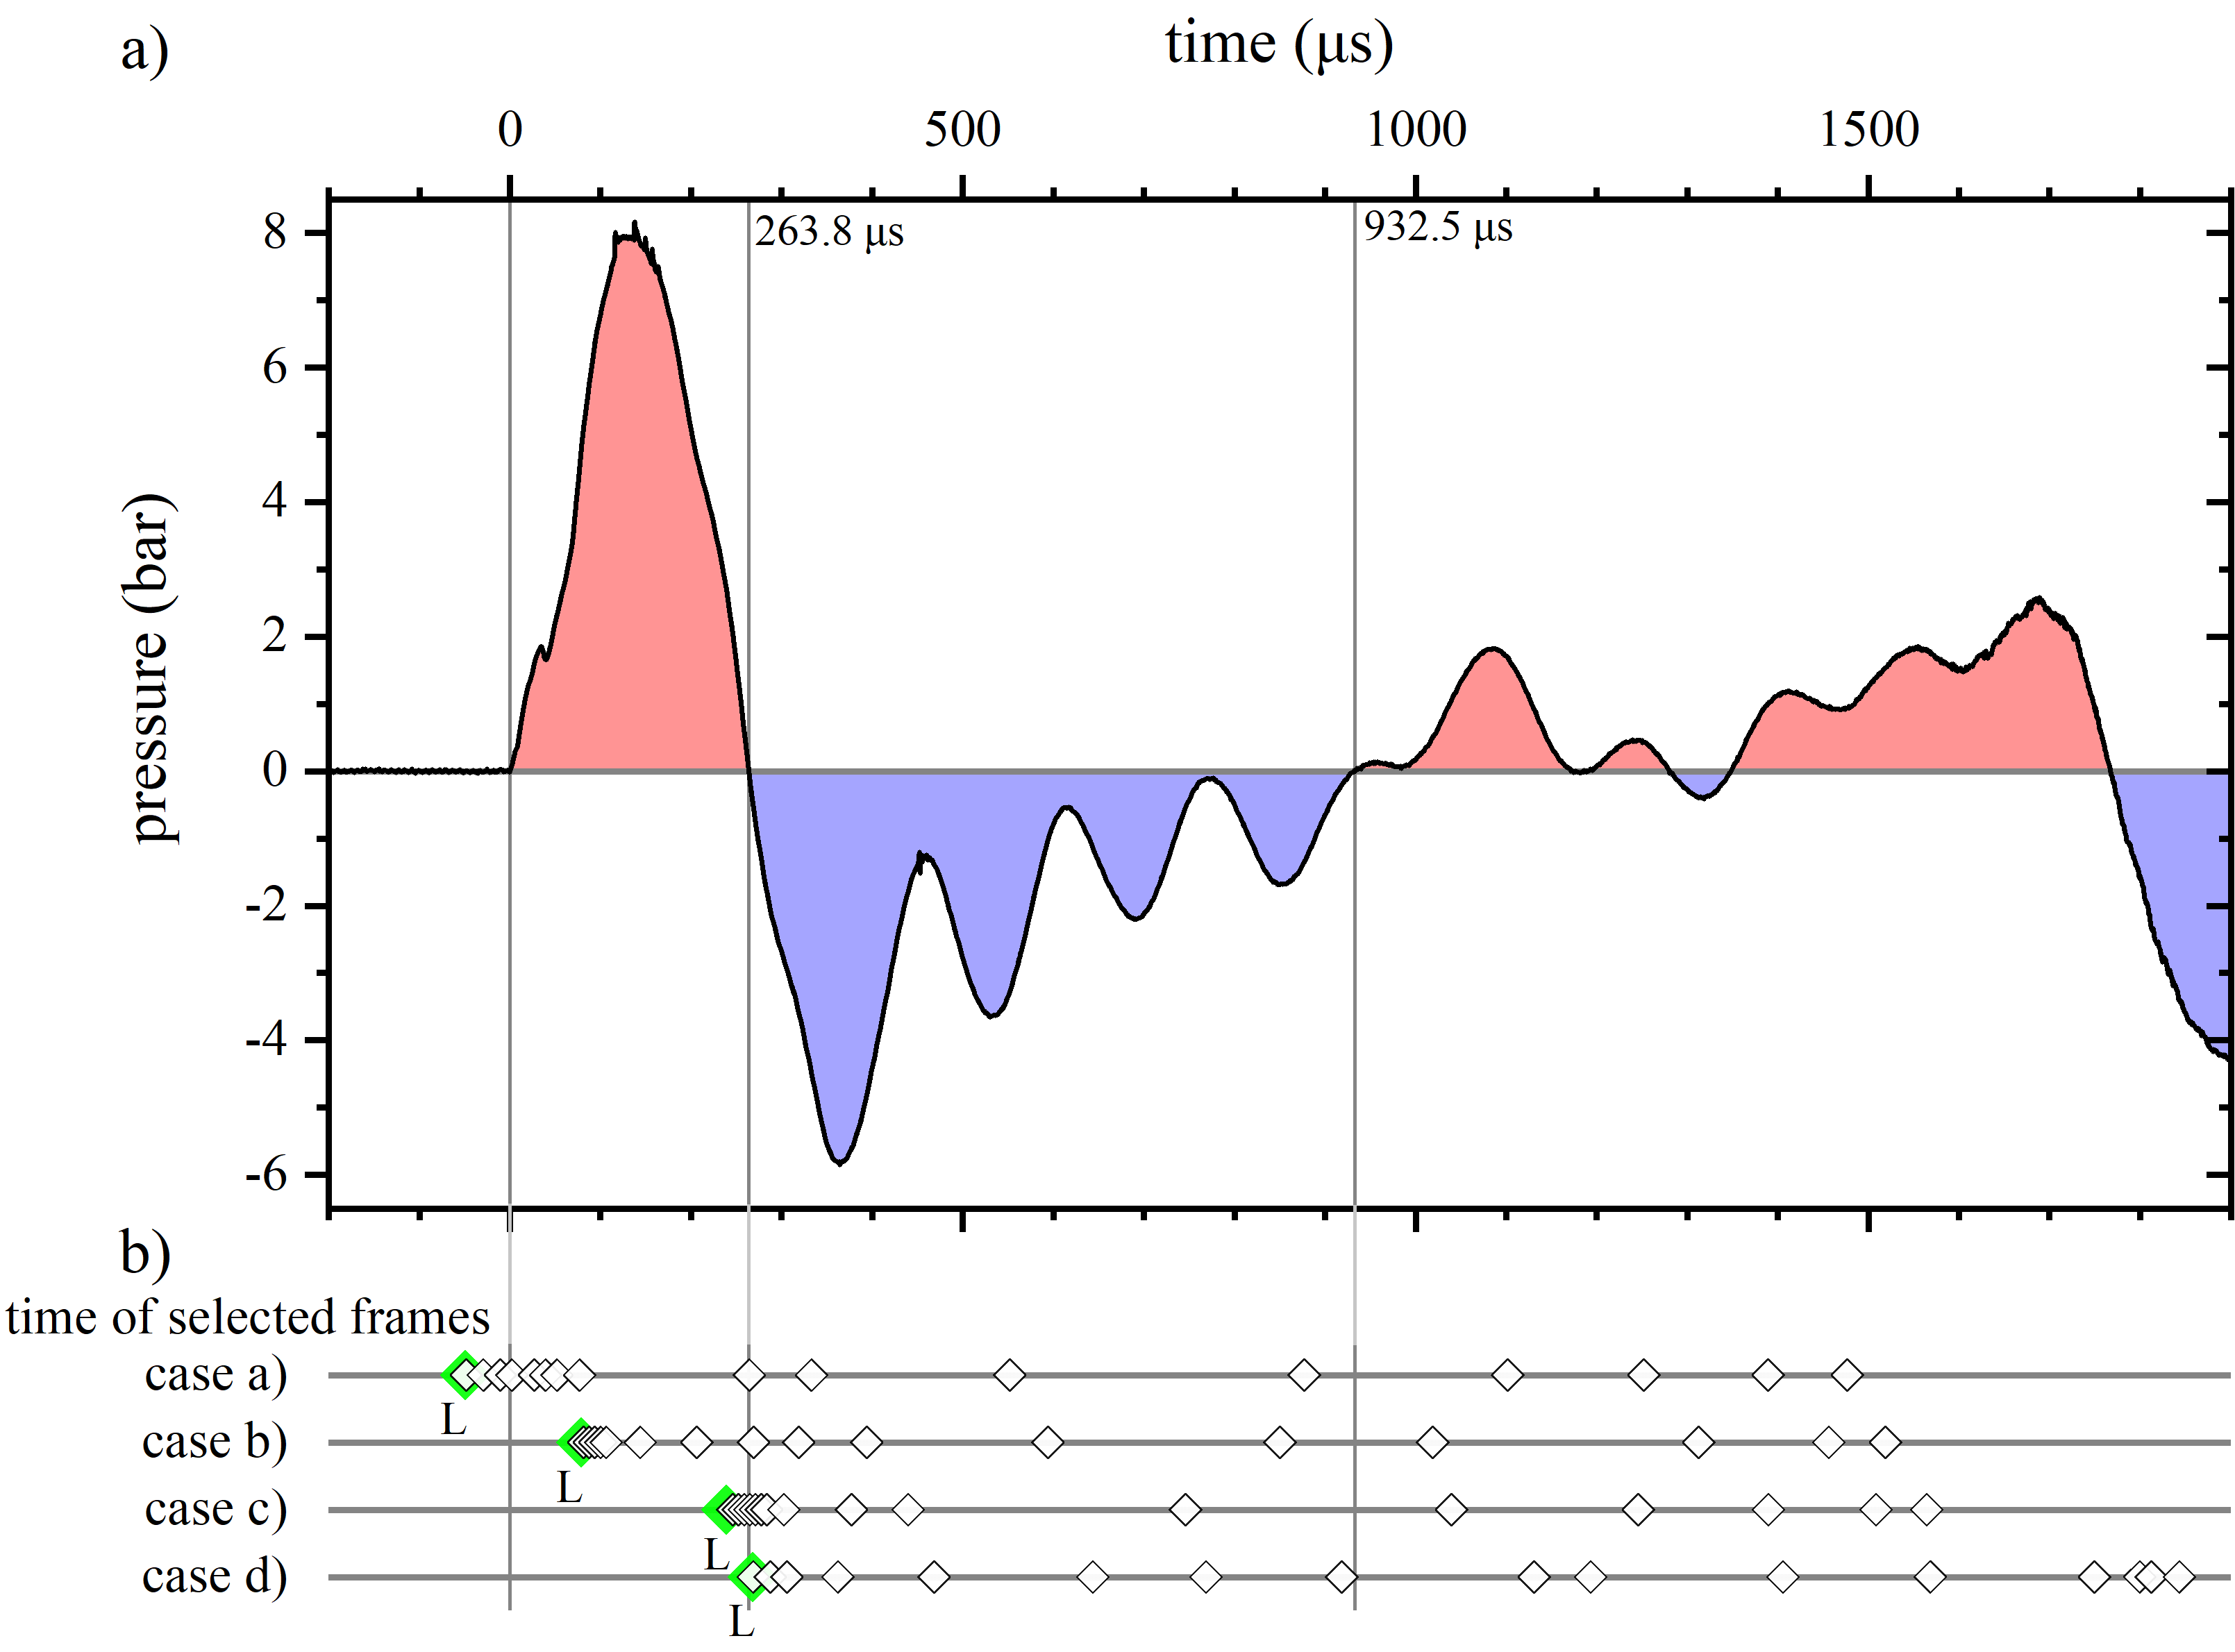
\includegraphics[width=1\linewidth]{img/fig5.11.png}
  \caption[压力波形与照片对应图]{ a) 即图\ref{fig:5.2} 压力波形图。b) 图 \ref{fig:5.13}
中图的时间线。每帧用空心菱形$\diamond$标注。绿色实心菱形并以``L''标注的是该案例的激光入射时间。}
  \label{fig:5.11}
\end{figure}



\begin{figure}[H]
  \centering
  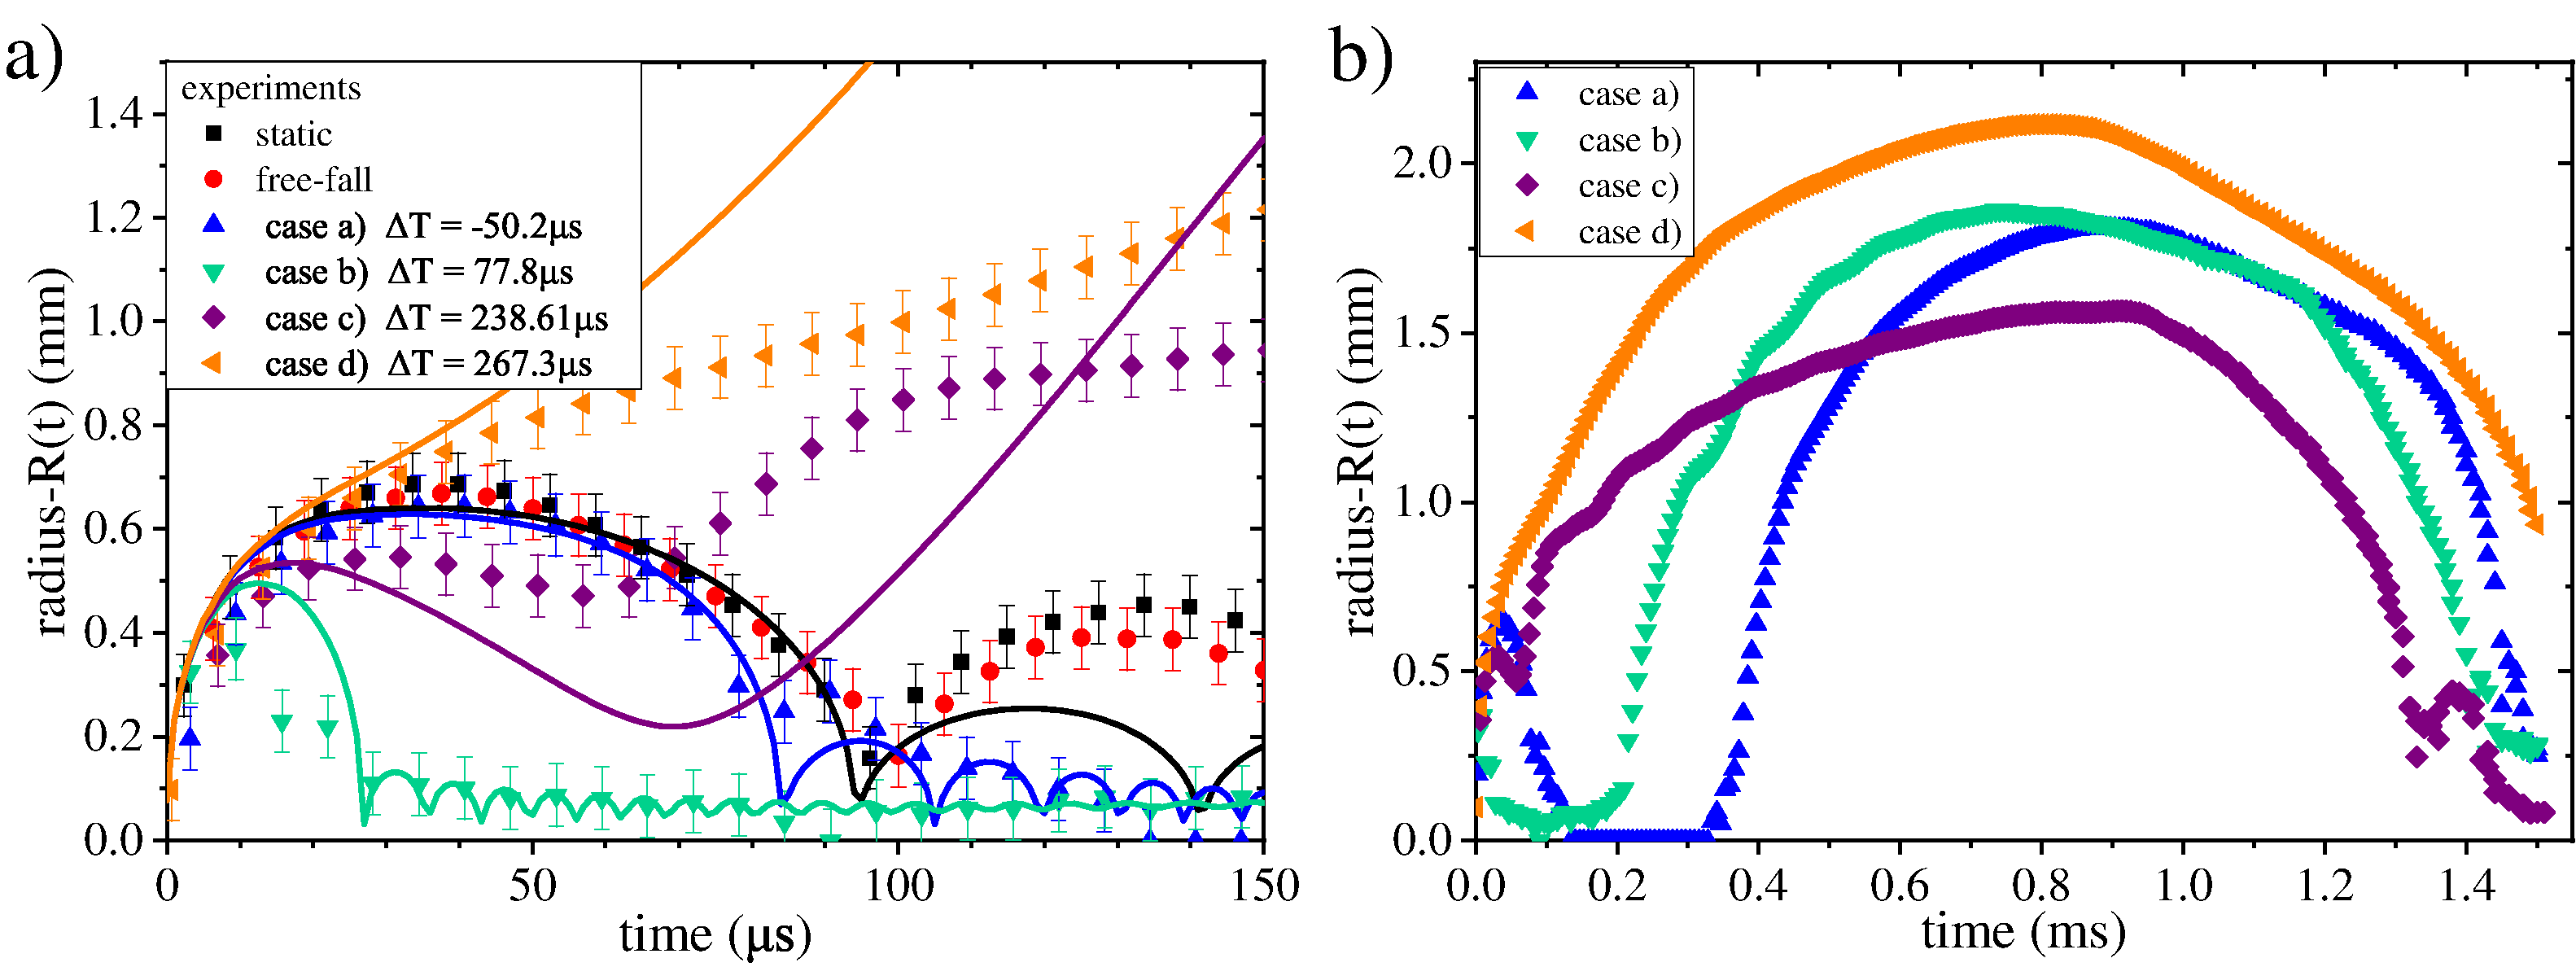
\includegraphics[width=1\linewidth]{img/fig5.12.pdf}
  \caption[典型案例的空泡半径-时间曲线图]{典型案例的空泡半径-时间曲线图。实验数据以符号图表示,而使用
Keller-Miksis
模型计算所得的半径使用实线表示。此处的半径是指等效半径$R (\text{t})$,即根据面积求得等面积圆形的半径。图中所包含的六种情形对应图
\ref{fig:5.9} 和图 \ref{fig:5.13}。误差棒表示了图像处理所致的不确定度。b)与
a)同样的实验,但延长其时间尺度到包含了后续空化云动力学过程。
}
  \label{fig:5.12}
\end{figure}



\begin{figure}[H]
  \centering
  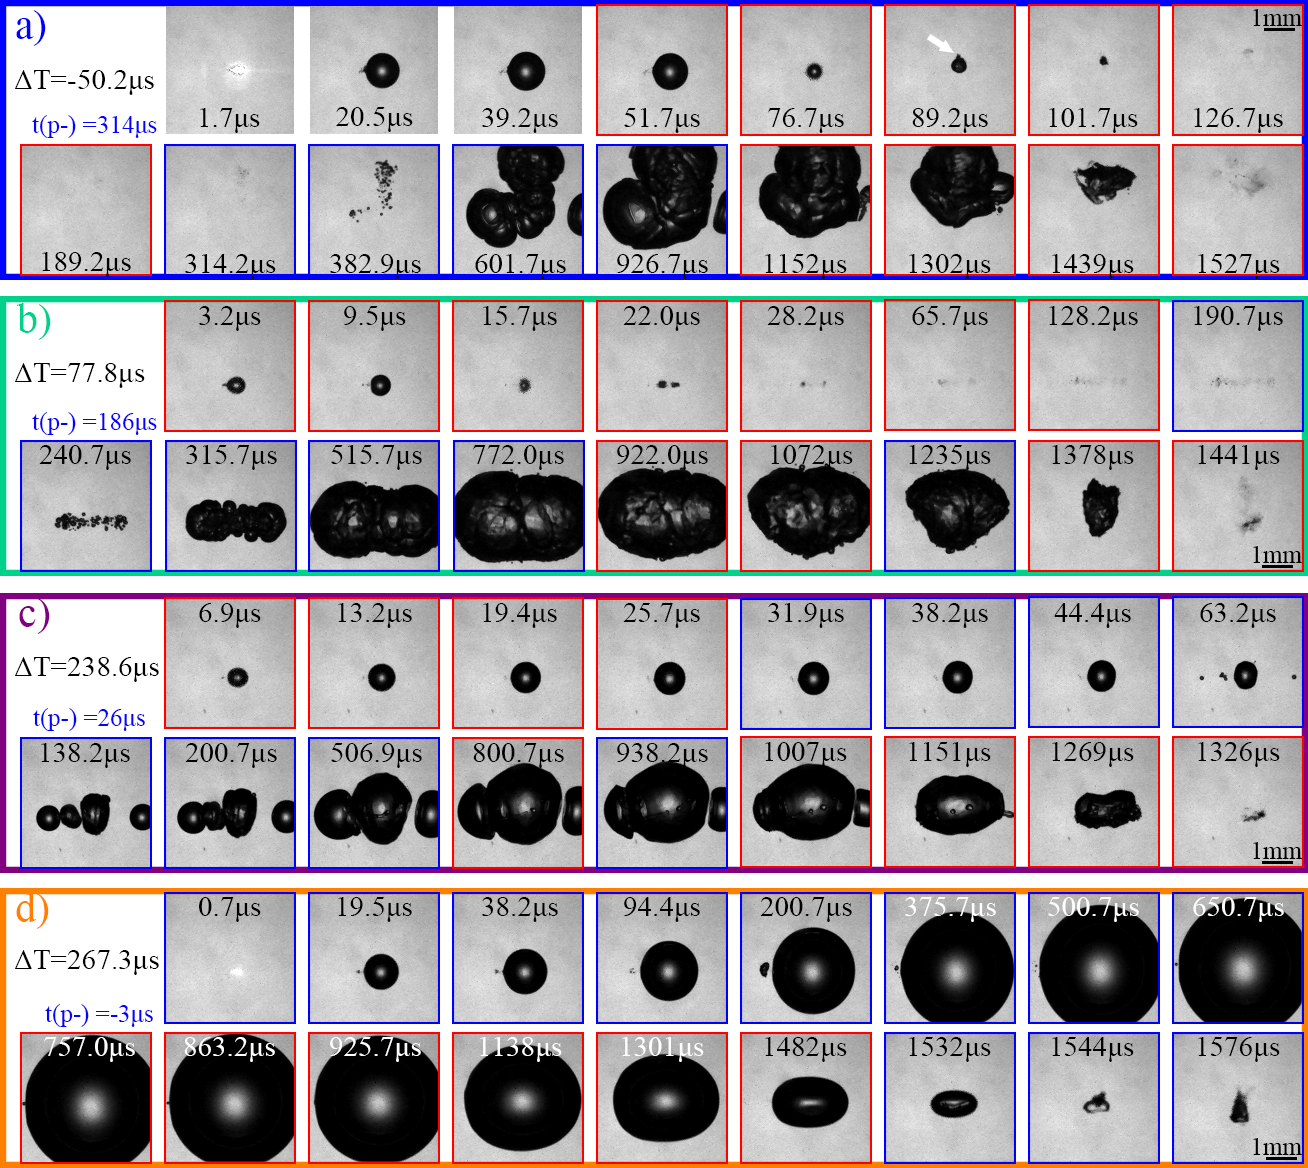
\includegraphics[width=1\linewidth]{img/fig5.13.png}
  \caption[产生于四种不同的压力波相位的空泡和空泡团簇动力学过程照片]{产生于四种不同的压力波相位的空泡和空泡团簇动力学过程照片。每一排以激光射入时的压力波相位区分,相位则用时间延迟
$\Delta T$
表示,也就是激光空泡产生时间减去压力波到达空泡位置的时间。压力脉冲在图
\ref{fig:5.11} a 中展现,对应的空泡半径演化在图 \ref{fig:5.12} 中展现。蓝色 $t (p-)$
标记显示了在空泡时间线上,每个案例中空泡所遭受的环境压力变为负压的时间点。每个案例的最后一帧标记了标尺。案例a),
$\Delta T=-50.2\,\mu \mathrm{s}$,显示了空泡在压力波到达之前产生,并在第一个脉动周期受影响的情况。案例b),
$\Delta T=77.8\,\mu \mathrm{s}$,显示了空泡在高压阶段产生的情景。案例c),
$\Delta T=238.6\,\mu \mathrm{s}$,显示了空泡产生在环境压从正压到负压的转换点附近的情景。
案例d),
$\Delta T=267.3\,\mu \mathrm{s}$,显示了空泡在负压阶段产生的情景。}
  \label{fig:5.13}
\end{figure}

在图 \ref{fig:5.13}中显示了四种不同脉冲相位产生的空泡。 图 \ref{fig:5.13}. a
显示了压力脉冲在空泡处于最大泡半径阶段时开始作用于空泡的情景。此种情形下,在竖直方向上存在压力梯度。高压加速了空泡的溃灭,继而减少了空泡的生存时间,见图
\ref{fig:5.12} 的 $R(t)$ 曲线。空泡的回弹也因为高压压迫而形成较小的空泡半径。在
$t=89.2\,\mu$ s,如图 \ref{fig:5.13}a
中箭头所示,可见清晰的逆重力方向,也就是顺着脉冲传播方向的射流形成。此射流的形成与压力脉冲的空间分布有关。我们使用如第三章中介绍的各向异性参数
${\zeta}=\left|\nabla p\right| R_{\text{max}} \Delta p^{-1}$
来辅助解释这个效应。据图 \ref{fig:5.11}. a 的斜率,代入水中声速
$c=1483\,ms^{-1}$,我们可以估算
$\left| \nabla p\right| \approx 436\,$
bar/m。从而,在空泡第一次溃灭,射流形成时, ${\zeta} \approx 0.30$
。这样的梯度比冲击波驱动的空泡溃灭要小得多\cite{sankin_shock_2005}。从而,射流在空泡的再膨胀阶段
$t=89.2\,\mu$ s.才明显可见。空泡在 $t=126.7\,\mu$ s
附近发生第二次溃灭。后续在 $t=314\,\mu$ s
张力波射入时,微小的空泡溃灭后残余混合气团,膨胀成为一群大空泡团簇。这群团簇持续生存至大约
$t=1500\,\mu$ s。

图 \ref{fig:5.13}.b 展现了空泡在正压相产生的时间序列照片(序列位置见图\ref{fig:5.12}.
b)。空泡在约 $t=9.5\,\mu$ s
时到达最大泡半径。而这个最大泡半径远远小于参照组的最大泡半径,即静压案例的
$R=0.69\,mm$。而且该情况下,高压而大大减小了空泡的生存时间,也大大减少了空泡后续脉动的持续时间和幅度。在这里,第一次溃灭时空泡在垂直方向上溃灭,由此形成水平排列的空泡碎片,这些碎片随着时间的推移而扩散。在溃灭过程中可能由于高压产生了一个水平流,运输空泡碎片。最后,空泡的残余混合气团在环境转为舒张相时,
$t=240.7\,\mu$ s
,被拉伸成为一群空泡团簇。这团空泡团簇,在溃灭时,因水平和竖直方向的相位差异,形成竖直方向的射流击穿空泡,并形成竖直分布的二次残余气团,如
$t=1441\mu$ s 所示。

在图 \ref{fig:5.13}. c
中,空泡产生于压力脉冲的正压相的终末阶段。此时,相比于参照组,其在产生和膨胀初期仍然受高压相的压迫,而使其最大半径及时间相应减小。而在空泡收缩时,由于环境压降低至舒张相,使空泡收缩收到抑制。继而没有产生溃灭,直接再膨胀。在再膨胀过程中(
$t>55\,\mu$
s),在空泡原位置的左右处产生了继发空泡。这是由于激光在当地传播过程中,电子密度不足以形成击穿,但是形成微小的体积相变。这些相变位置作为凝结核,在收到张力波作用后形成新的空化。由于这种激光和张力的双重作用,形成的随机空泡多数尺寸在分辨能力以下。但在激光路径高热区形成的这些空泡与原空泡碎片膨胀合并,在
$t=900\,\mu$ s 处达到最大泡半径,并在 $t=1300\,\mu$ s 时溃灭,参考图\ref{fig:5.12}
。

图 \ref{fig:5.13} 中,案例 a) 到 c) 都受到高压相影响,而案例 d)
则是空泡产生于张力相。张力持续了 $668\,\mu$ s
。在此期间空泡膨胀成为一个相比于静态空泡尺寸非常大的单体大体积空泡,即
$R_\mathrm{max}=2.22\,$ mm 与 $R_\mathrm{max}=0.7\,$ mm 对比。在
$t=932.5\,\mu$ s
时,压力重新转为正压,此时空泡开始收缩。空泡溃灭时是一个凸出的椭圆体,其次轴与重力方向一致。此处形状来源于叠加边界和压力波的双重作用。由于试管壁的存在,边界阻碍了水从侧面的流入补充空泡收缩让出的空间。后续正压在竖直方向上形成压力梯度,助长了这种形状。双重作用形成的压力梯度诱发了向上的喷射流,在图
\ref{fig:5.13}.d 中 $t=1544\,\mu$ s 处很明显。

除了实验数据,图 \ref{fig:5.12}
显示了数值模拟的各自半径。一般地,实验和数值曲线在第一次振荡中是相当一致的。可以观察到后续的差别,这主要是由于忽略了空泡到空泡团簇之间的破碎过程,以及从团簇到球形空泡的近似。同时液域的圆柱形封闭限制了实验中空泡的膨胀和收缩,这一点在这个简单的计算模型中没有考虑。


\subsection{空泡对压力波的相位响应}

图 \ref{fig:5.14}. a 和 \ref{fig:5.14}.b 分别显示了空泡对 $\Delta T$
的响应的实验和模拟结果,$\Delta T$
是空泡产生时刻和脉冲压力通过空泡点的时间差 $\Delta T$ 。其中,空泡半径
$R(t)$ 是用颜色编码的。对于 $\Delta T=0$
的阶段,空泡是在脉冲压力波到达激光焦点的时刻产生的。$\Delta T$
的负值指的是在压力波通过前产生的空泡。虚线表示压力波到达空泡位置的时间。因此,从这条线开始,经过一段时间后,发现一个蓝色的区域,表示各自的空泡压缩。然而,对于
$250\,\mu$ s 和 $200\,\mu$ s
之间的阶段,第一次和第二次膨胀发生在压力脉冲通过之前。因此,空泡动力学基本与
$\Delta T$
无关,这个阶段范围内的空泡显示出基本相同的动力学,例如,它们都在
$100\,\mu$ s 左右崩溃。然而,在压力波通过前 $100\,\mu$ s
产生的空泡的反弹却受到影响。在更接近压力波通过的地方产生的空泡,例如
$\Delta T>-50\,\mu$
s,显示出第一个空泡膨胀的强烈减弱,只有微小的反弹。对于
$\Delta T>100\,\mu$ s(图中右下角的 $t>140\,\mu$
s),由于稀疏波的通过,空泡再次膨胀。

\begin{figure}[H]
  \centering
  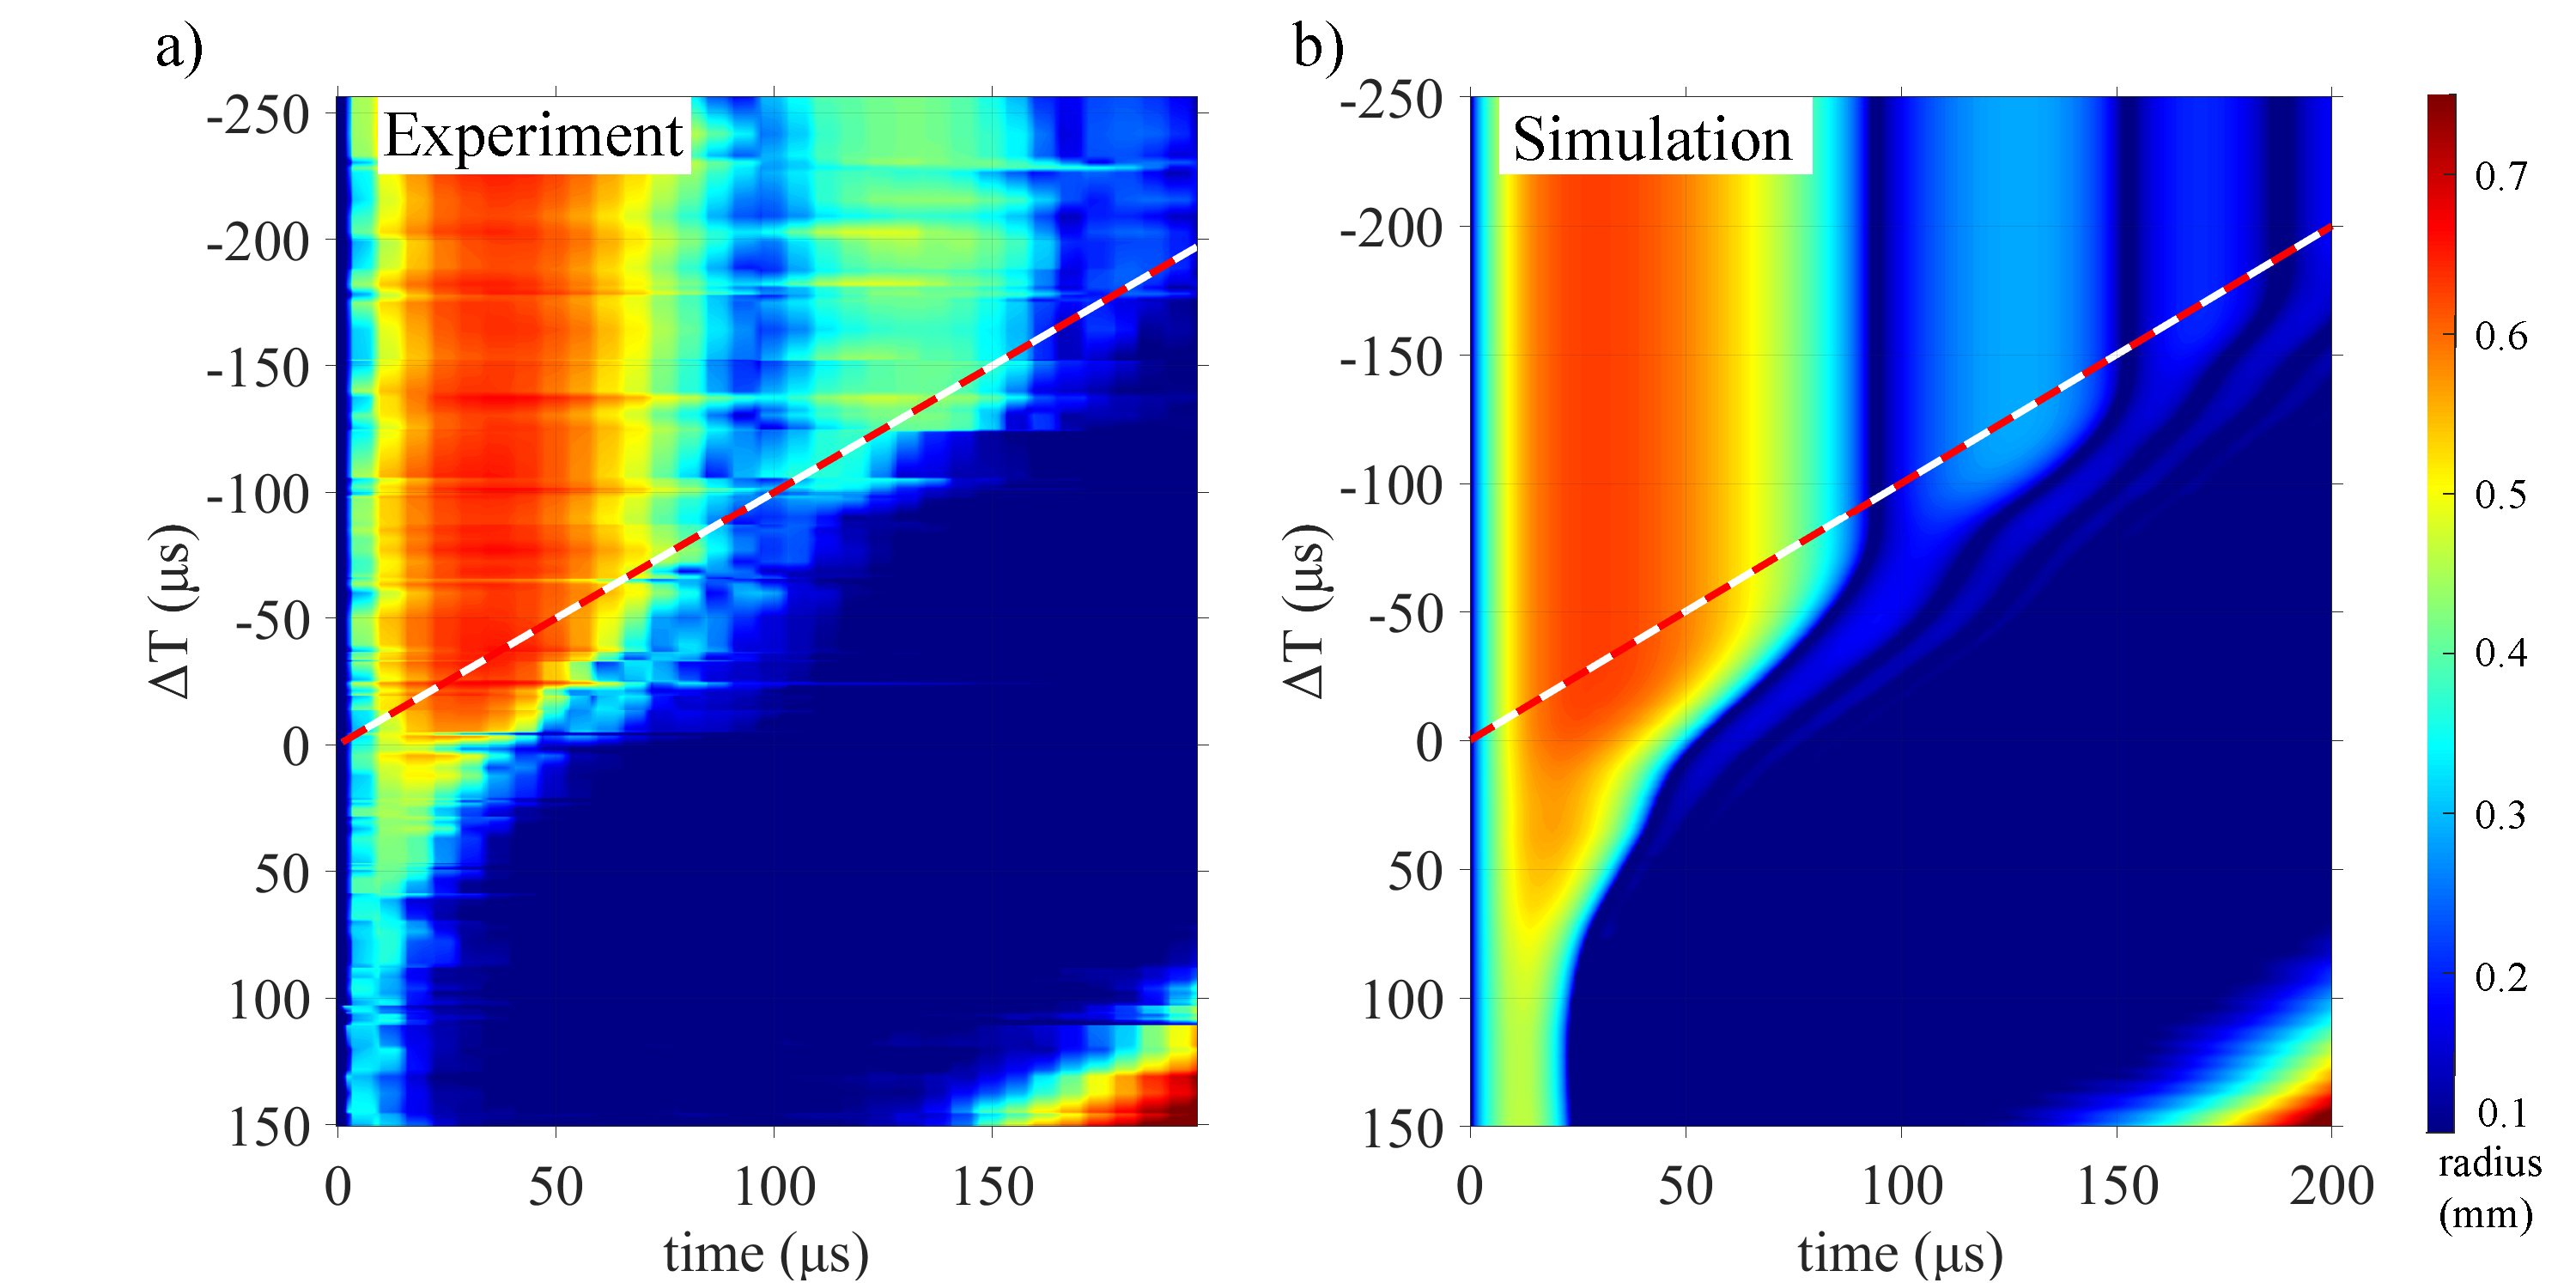
\includegraphics[width=1\linewidth]{img/fig5.14.pdf}
  \caption[空泡生成时间与冲击波射入时间差$\Delta T$对应的空泡半径$R (t)$演化]{空泡生成时间与冲击波射入时间差$\Delta T$对应的空泡半径$R (t)$演化。时间零点$t=0$
,指空泡诞生时间。竖直轴是空泡产生时延,$\Delta T$,此处负值指空泡先于压力波作用产生。红白间断线代表了压力波开始时间。a)
实验结果。 b) K-M 与测得压力波结合计算所得的空泡响应。
}
  \label{fig:5.14}
\end{figure}

现在让我们把测得的空泡响应与图\ref{fig:5.14}. b
中的模拟结果进行比较。对于所有的模拟,Keller-Miksis 模型的初始条件是
$R(t=0)=54\,\mu$ m 和 $\dot{R}(t=0)=1280\,$
m/s,平衡半径,即不可凝结的气体量,是 $R_n=90\,\mu$
m。详情请见本作第二章。总的来说,我们发现实验和球形空泡模型之间有良好的定性和定量的一致性。特别是,随着
$\Delta T$ 的增加,空泡生存时间的缩短被很好地再现了。另外,在图 \ref{fig:5.14}.b
中右下角区域的大 $\Delta T$ 和大 $t$
的空泡开始重新膨胀的现象在模拟中得到了证实。良好的一致性也证明了空泡成核和脉冲压力产生的实验是高度可重复的。

模拟和实验之间有一些差异,在反弹中可见。在实验中,这些反弹持续的时间约为20\%。这可能是由于与模拟相比,实验中的溃灭较弱。实验中较弱的溃灭通过声发射消散的能量较少。因此,更多的能量可用于再膨胀,空泡膨胀到一个更大的半径。模拟溃灭辐射更多能量的原因可能是由于理想绝热气体的热力学简化导致,但也有试管的封闭几何形状的原因,这在模拟中没有考虑到。试管的几何形状阻止了球形汇聚流,与较大的比色皿相比,可能会导致较小的液体速度。

\subsection{空泡团簇脉动的脉动行为}
在压力波实验中,我们看到,除了空泡溃灭的时间缩短外,当脉冲压力的稀疏波部分与激光诱导致空泡相互作用时,可以诱导产生大体积空泡和空泡团。

在这里,我们在图 \ref{fig:5.15} 中,更详细地分析大体积空泡和空泡团作为相位
$\Delta T$ 的函数的动力学,使之涵盖了与之前的图 \ref{fig:5.14}相比更多的
$\Delta T$ 和时间 $t$ 的范围。 图 \ref{fig:5.15}. a
显示了实验的半径时间数据,图\ref{fig:5.15}. b
显示了模拟的空泡动态。请注意两图中不同的色标范围。左上方的图 \ref{fig:5.15}.
a,即小 $\Delta T$ 和小 $t$,是对之前图 \ref{fig:5.14}. a
的再现。正压的开始用红色虚线表示,标记为 $p+$。图\ref{fig:5.15}
最突出的特征是在 $p-$ 线之后形成的大红球。它的最大值在张力阶段开始后约
$500\, \mu s$ 达到。在 $p+$ 和 $p-$
线之间的淡蓝色区域表示只有非常小的空泡或根本没有空泡可见。其中仍然有空化核存在,一旦舒张波到达就会膨胀成空泡。这个区域在图
\ref{fig:5.15}.a 中被称为
``空泡群'',因为这里有多个空泡膨胀并合并。这里绘制的等效半径必须被理解为一个近似的半径。它是通过整合高速帧中被空泡覆盖的像素区域而得到的。通过假设是一个单一的投影空泡这个面积被转换为等效半径。

形成空泡团的多空化核的起源是激光诱导的空化空泡在其第一次和以后的溃灭过程中形成的小空泡碎片。同时,形成的微观气体碎片,会因扩散以及溶解的原因而减小。但这个溶解时间比$p+$和$p-$之间的时间跨度要长得多,也就是说,一旦稀疏波到达,这些碎片就会作为空化核。

\begin{figure}[H]
  \centering
  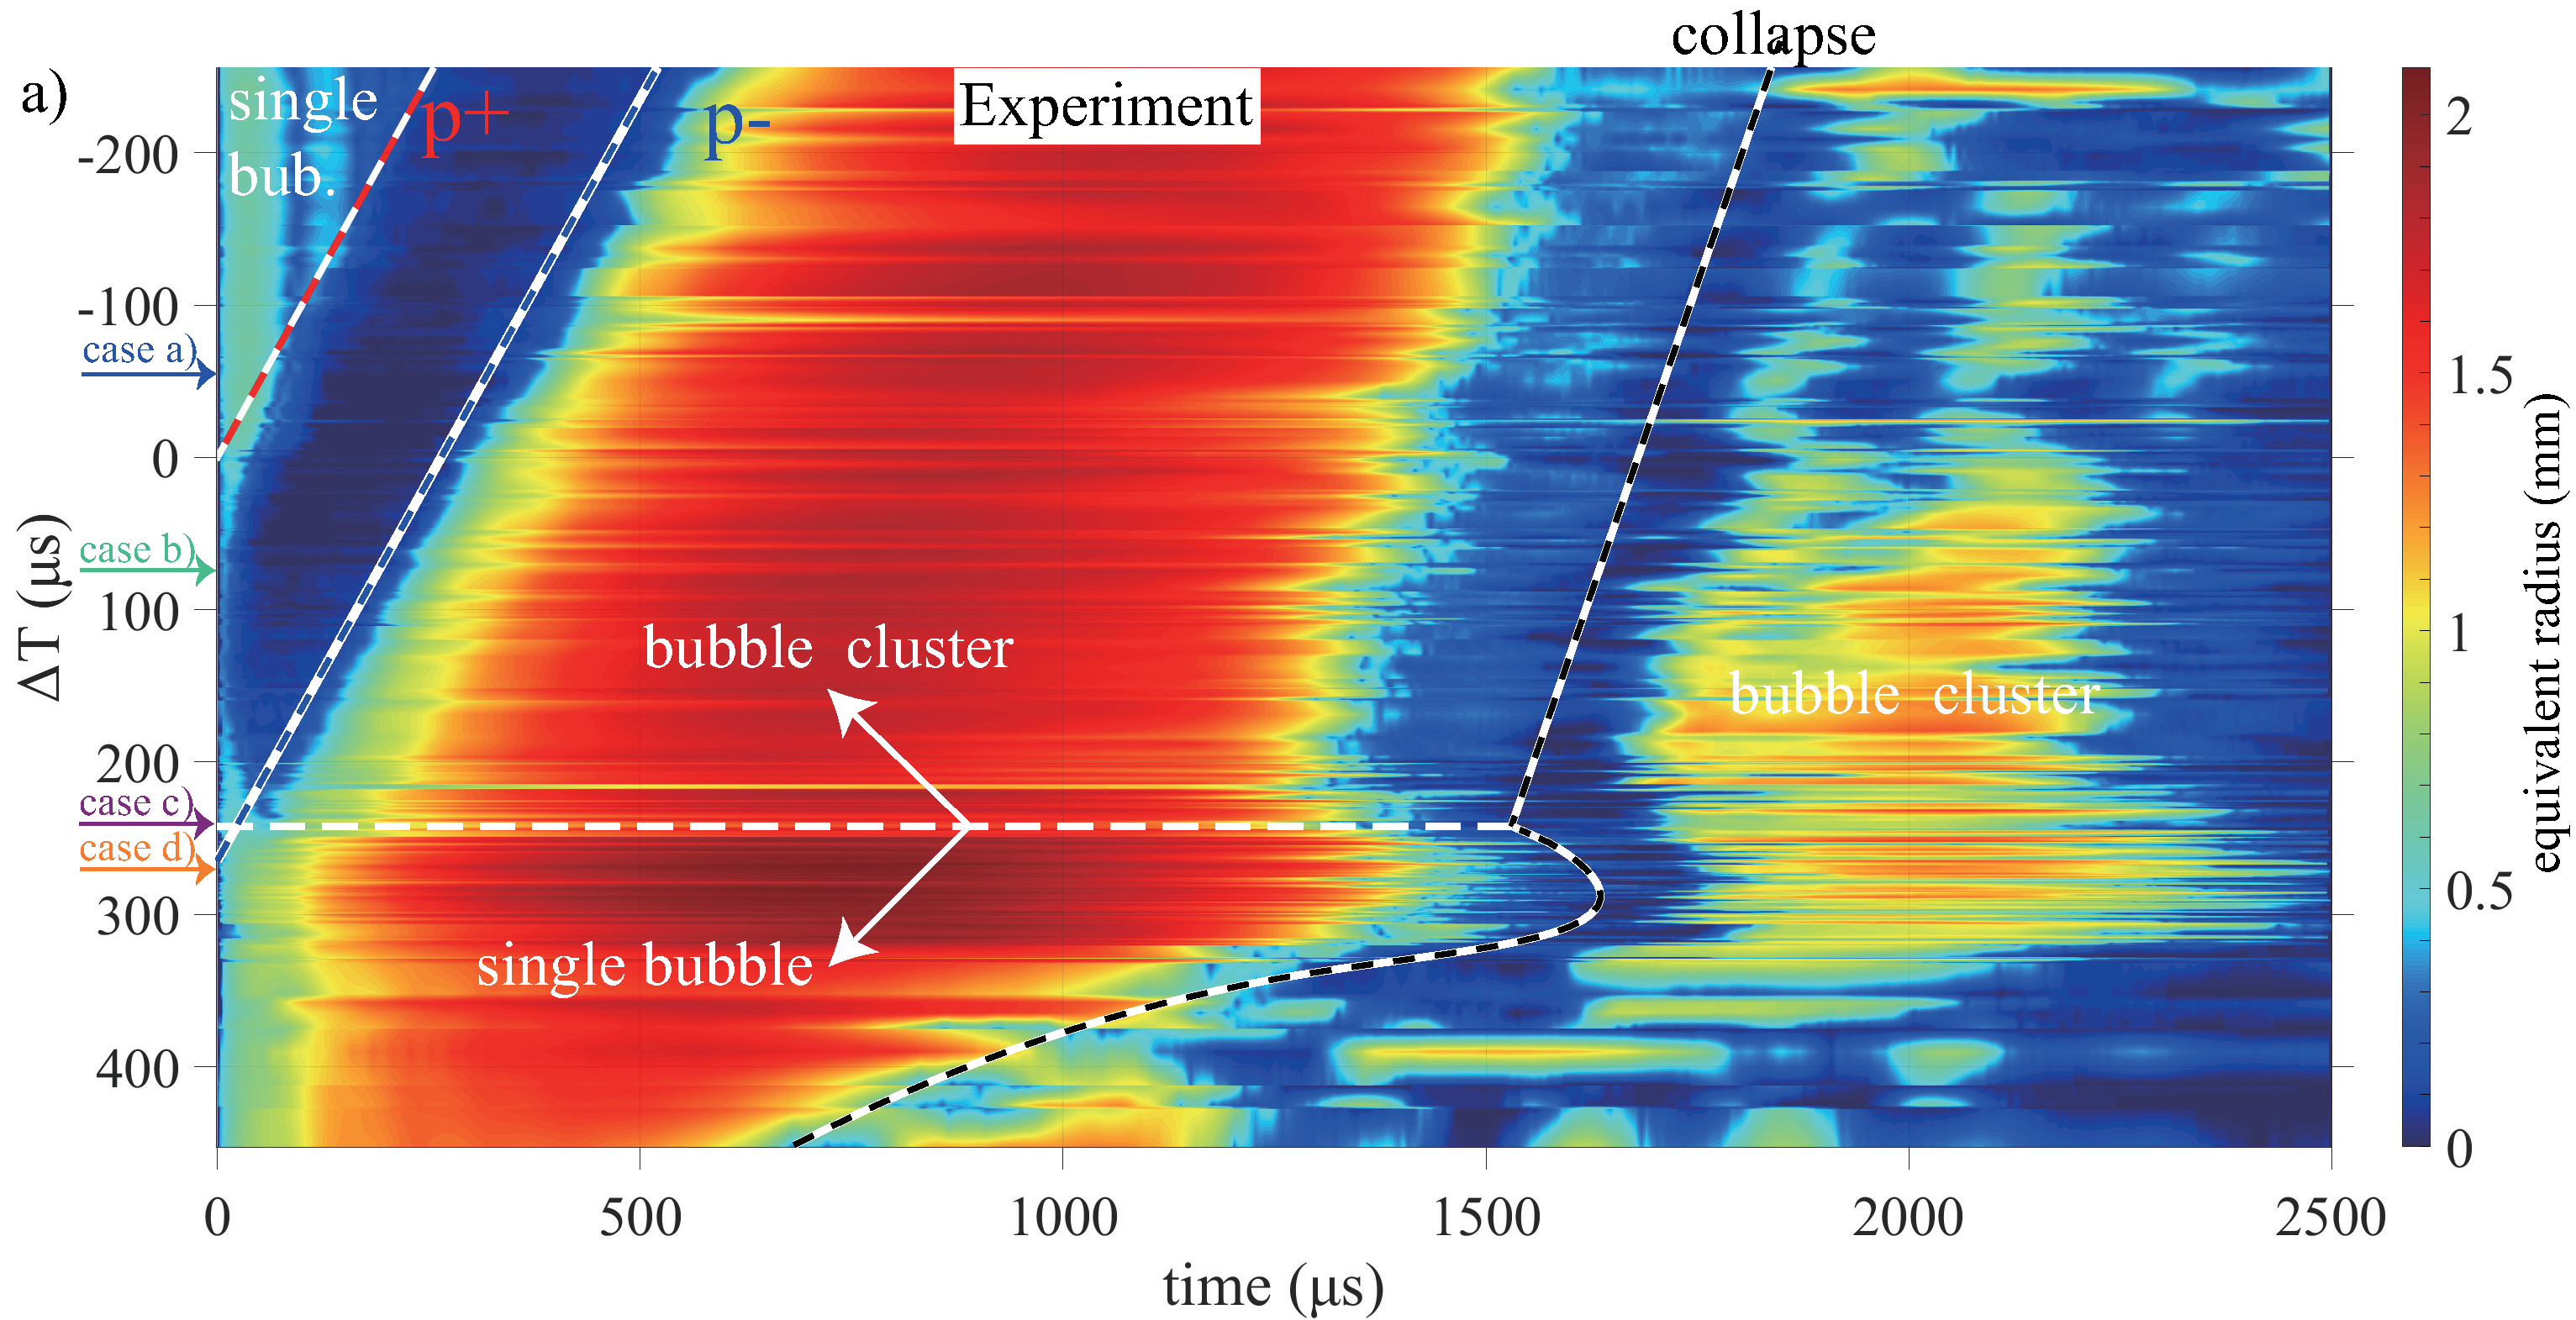
\includegraphics[width=1\linewidth]{img/fig5.15a.pdf}
  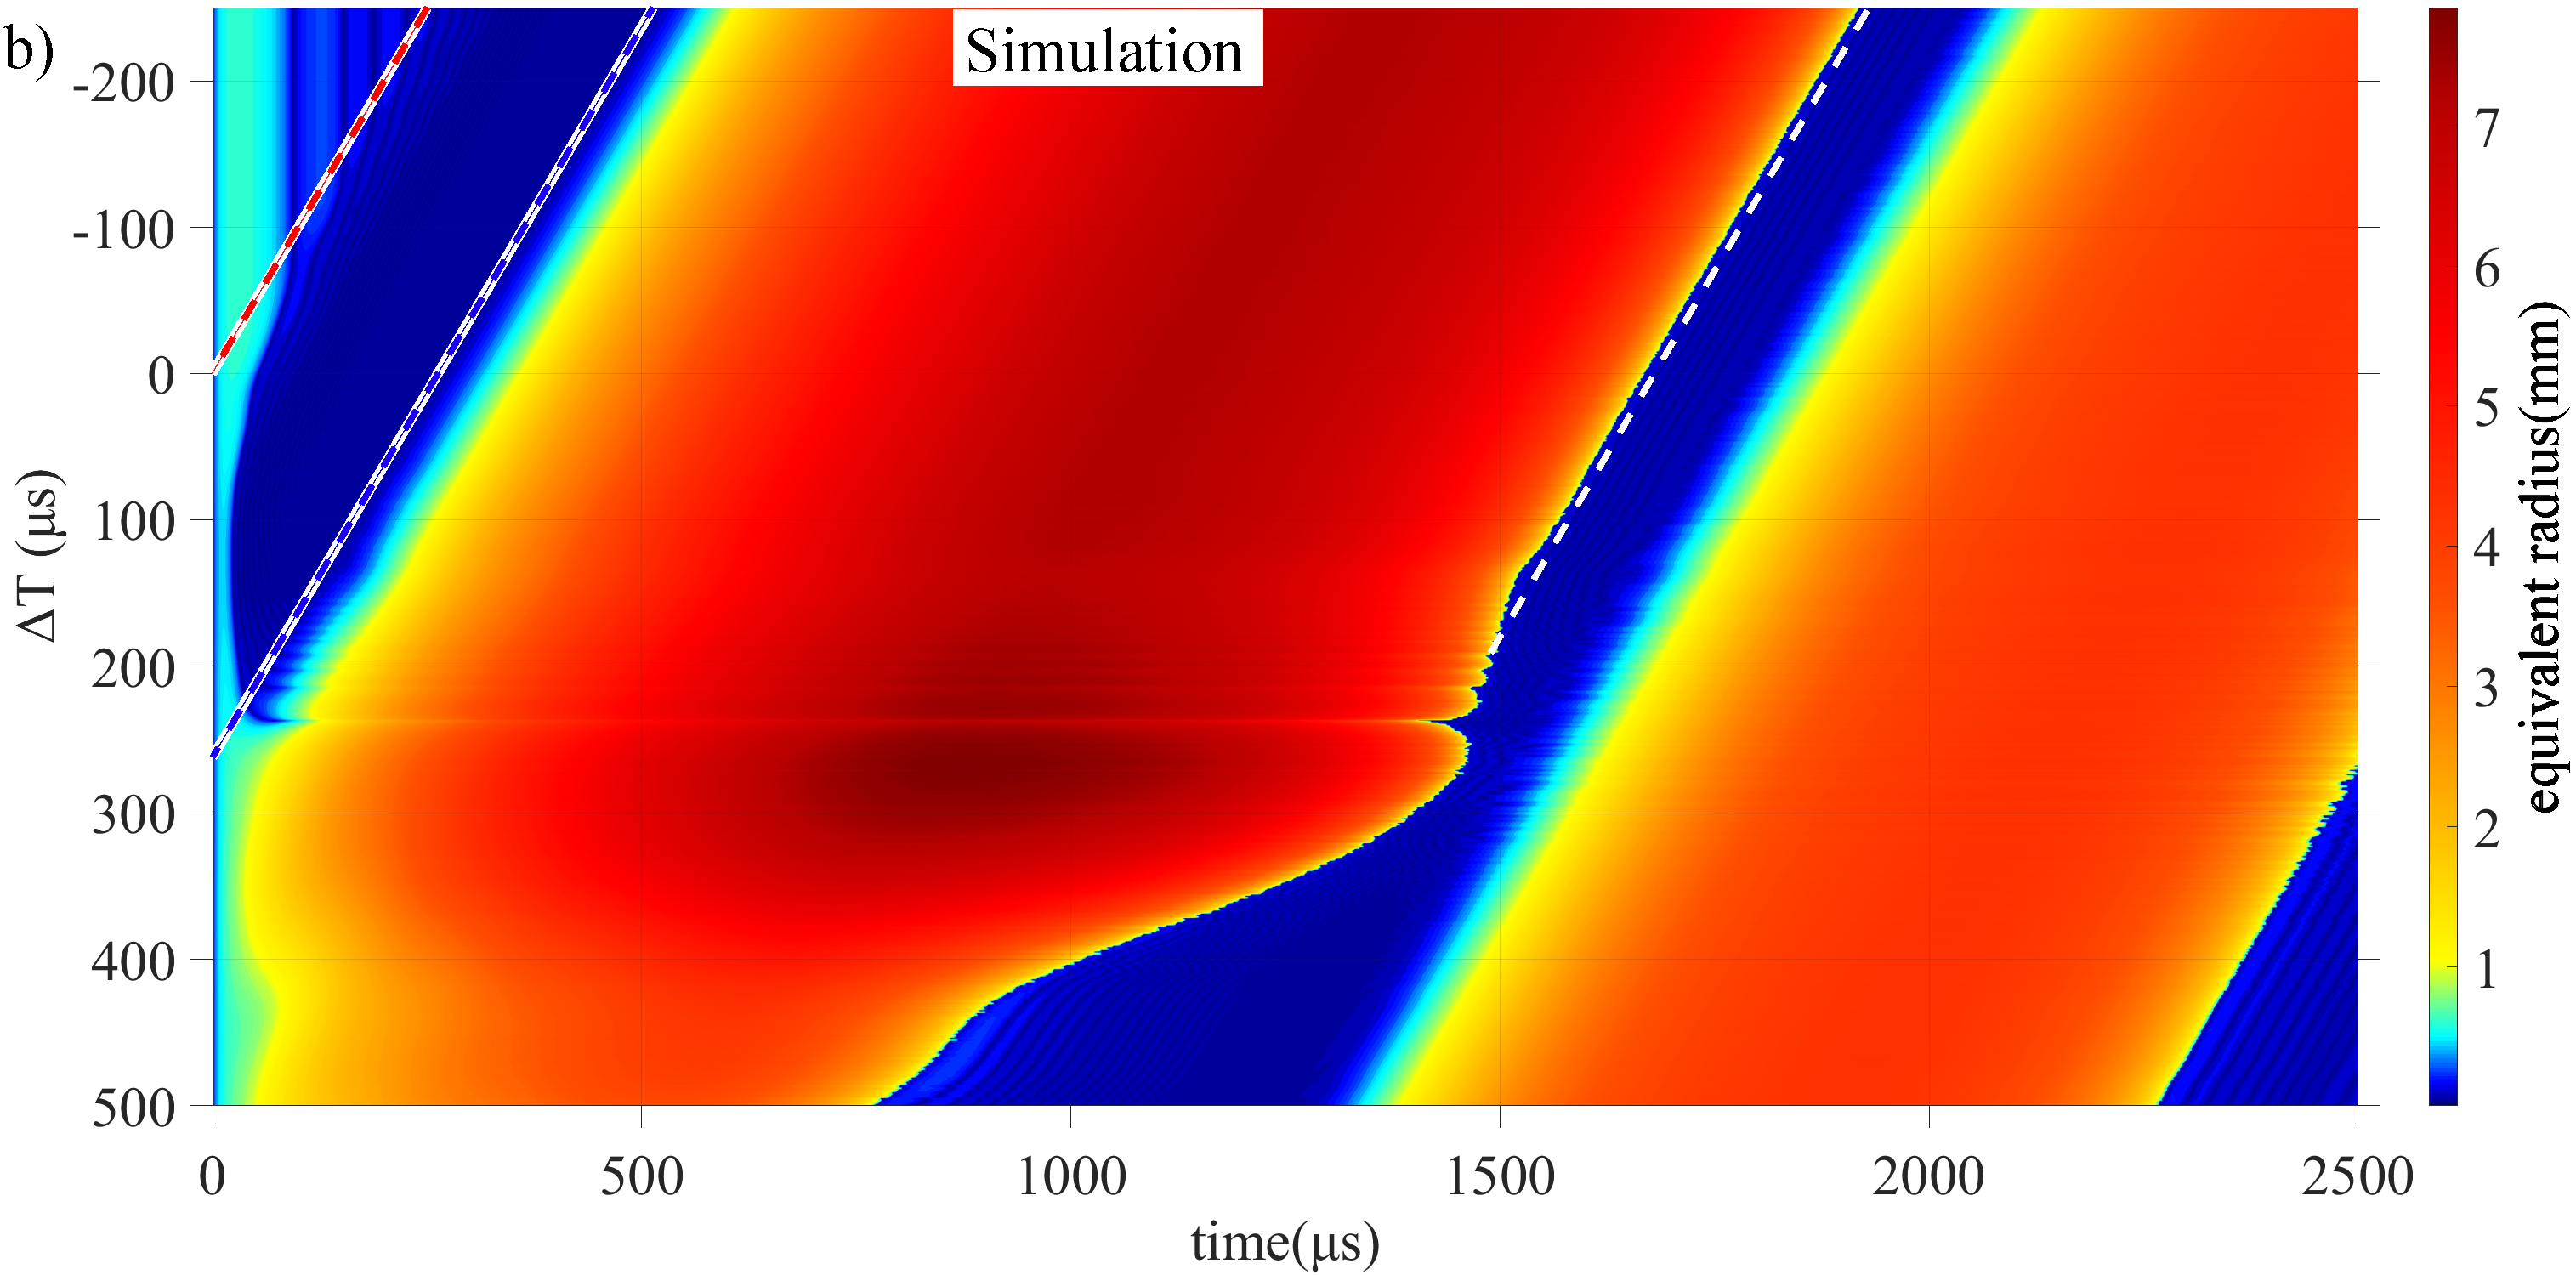
\includegraphics[width=1\linewidth]{img/fig5.15b.pdf}
  \caption[实验和 K-M
模型计算结果比较。]{实验和 K-M
模型计算结果比较。与图 \ref{fig:5.14}
具有相同的轴内容设置,但具有更长的包括空泡团簇过程的时间尺度。a)
实验获得的$R (t)$。图 \ref{fig:5.13}中显示的典型案例在 y 轴上特殊标识。b)
Keller-Miksis 模型计算获得的空泡响应,脉动半径$R (t)$。K-M
模型获得了较大的空泡半径,图色标尺作了截止处理,以获得更好的对比效果。红白间断线代表了压力波到达空泡位置的零时刻。蓝白剪断线代表了压力波转化为张力波的时刻。黑白间断曲线勾勒出了空泡溃灭时刻,而白色虚线将图划分为空泡团簇区域和单空泡区域。}
  \label{fig:5.15}
\end{figure}

图中提出的四种情况的 $\Delta T$ 的阶段在图 \ref{fig:5.13}纵轴上标出。案例 a)
和案例 b) 呈现较早的溃灭和空泡碎片重新膨胀成团的结果,而案例 c) 和案例
d) 则显示为单个空泡的膨胀。情况
c)特别有趣,因为在这里,正压作用在空泡上的时间很短,不足以诱发完全崩溃,空泡在收缩一段时间后,在负压的作用下重新膨胀为一个大体积空泡。有趣的是,这个单一空泡的生存时间明显长于以稍短的阶段
$\Delta T$ 产生的空泡群。

当空泡完全在张力阶段引入时(见 $\Delta T\geq 263.8\,\mu$
s),空泡扩展为一个更大的单一空泡,具有更长的第一次振荡周期,在这里它被张力阶段的持续时间所限制。这一点通过增加相位
$\Delta T$
时第一次振荡持续时间的减少得到证实。从空泡群到大的单个空泡的过渡发生在情况
c) 周围,见图 \ref{fig:5.15}.a 中的水平虚线。

实验和数值数据显示了类似的定性行为,尽管数值模型只考虑了单一的球形空泡。在实验中,空泡团机制的溃灭时间被高估了。我们将此归因于试管边界的影响,限制了实验中空泡的膨胀。因此,空泡没有像模拟中那样膨胀,在模拟中它们也较晚崩溃。
然而,一般认为,模拟中的空泡膨胀了大约两到三倍,这将对应于至少两倍的溃灭时间。但在实验中,溃灭时间最多只缩短了20%。这可以解释为,在空泡与容器大小相近的受限几何形状中,空泡的生存时间也会延长\cite{quinto-su_cavitation_2009}。

空泡的最短生存时间存在于 $80\,\mu$ s $\,\le Δ T\le 160\,\mu$
s,此时其被减少到小于 $20\,\mu$
s。这一发现在模拟中得到了再现。然而,对于空泡团的溃灭,我们看到实验和模拟之间的一致性较差。在模拟中,图
\ref{fig:5.15}.b,在第一次大膨胀之后,所有的空泡都以同样的方式重新膨胀,只是被
$\Delta T$ 的相位转移了。在实验中,只有在 $150,\mu$ s 和 $300,\mu$
s 之间的 $\Delta T$
观察到相当大的再膨胀。这清楚地表明,用这个简单的模型只能在一定程度上模拟团簇的动态。另外,再膨胀在很大程度上是由空泡内容物含量决定的。该模型没有考虑到质量运输、冷凝和蒸发。这对主要含有水汽的空泡来说特别重要,因为这里就是这种情况
\cite{akhatov_collapse_2001}.。

当负压在第二个振荡周期开始时,甚至在溃灭的很晚阶段,脉冲压力波仍然压缩第一周期的空泡,反射的溃灭冲击波也能影响它的反弹,这在计算中都没有考虑。越来越大的负压直接使第二个循环的空泡反弹。这在实验和计算结果中都很清楚。

在正压相的最后阶段产生的空泡脉动有着逐渐增大的脉动周期。这是由于空泡初始环境压力的降逐渐降低而导致的。
同时,空泡溃灭和团簇重生的时间相交,也就是空泡团簇重生机制转变为空泡自身反弹机制发生在$\Delta T=234\,\mu s$左右,即空泡产生于正压的很晚阶段,其中空泡的第一周期时间小于静态第一振荡时间。

空泡不能达到其可实现的最大半径和生存时间,即使它在溃灭阶段内遭受负能量。
我们认为能量损失发生在空泡产生的初始阶段,这也是与空泡相互作用的急剧变化的正压冲力的阶段。脉冲释放了新生空泡的能量,使其最大半径变小,例如,在$\Delta T=234\mu s$的情况下,空泡最大半径在$20\mu s$时约为6mm。
在空泡生成的$30\mu s$后,它遭受了负压,但其仍在收缩,直到$80\mu s$。此处,$\Delta T=234\,\mu s$是一个分水岭,正如数值结果所显示的,在这之前,负压不能在空泡溃灭之前使其半径回升。其后,空泡会在其溃灭之前反弹。由于溃灭抵消了张力,空泡失去了能量,所以它的生存时间明显缩短,这在图像上显示为一个缺口。
正如前面提到的案例$\Delta T=238\,\mu s$所示,在这个阶段产生的空泡并没有达到静态的最大半径,在缓慢收缩后,它又反弹了。
由于不充分的溃灭,空泡的能量在开始重生的时候会有一点衰减。
在这种情况下,少许衰减的空泡能量加上高负压使得空泡半径变的更大。

在后期负压阶段产生的空泡,在张力波的拉伸作用下,直接膨胀到空泡簇的最大半径,而不经过任何收缩。
在这种情况下,空泡有更多的能量。
与以前的情况相比,它使泡群的最大半径更大,生存时间更长,如图中的凸起所示。
随着空泡产生的时间继续在压力波时间正方向上移动,空泡生存时间和最大半径减少。
这是由于环境压力在达到最大值之前越来越早地上升到最初的正常水平。

尽管如此,第二个振荡周期也发生在空泡群上。但由于残留的溃灭的空泡气体比较分散,由于大体积空泡有更多的能量产生更密集的现象,很难区分和计数代表分散的小空泡的像素。所记录的新的反弹团簇是由多种来源引起的,这里不作讨论。

\begin{figure}[H]
  \centering
  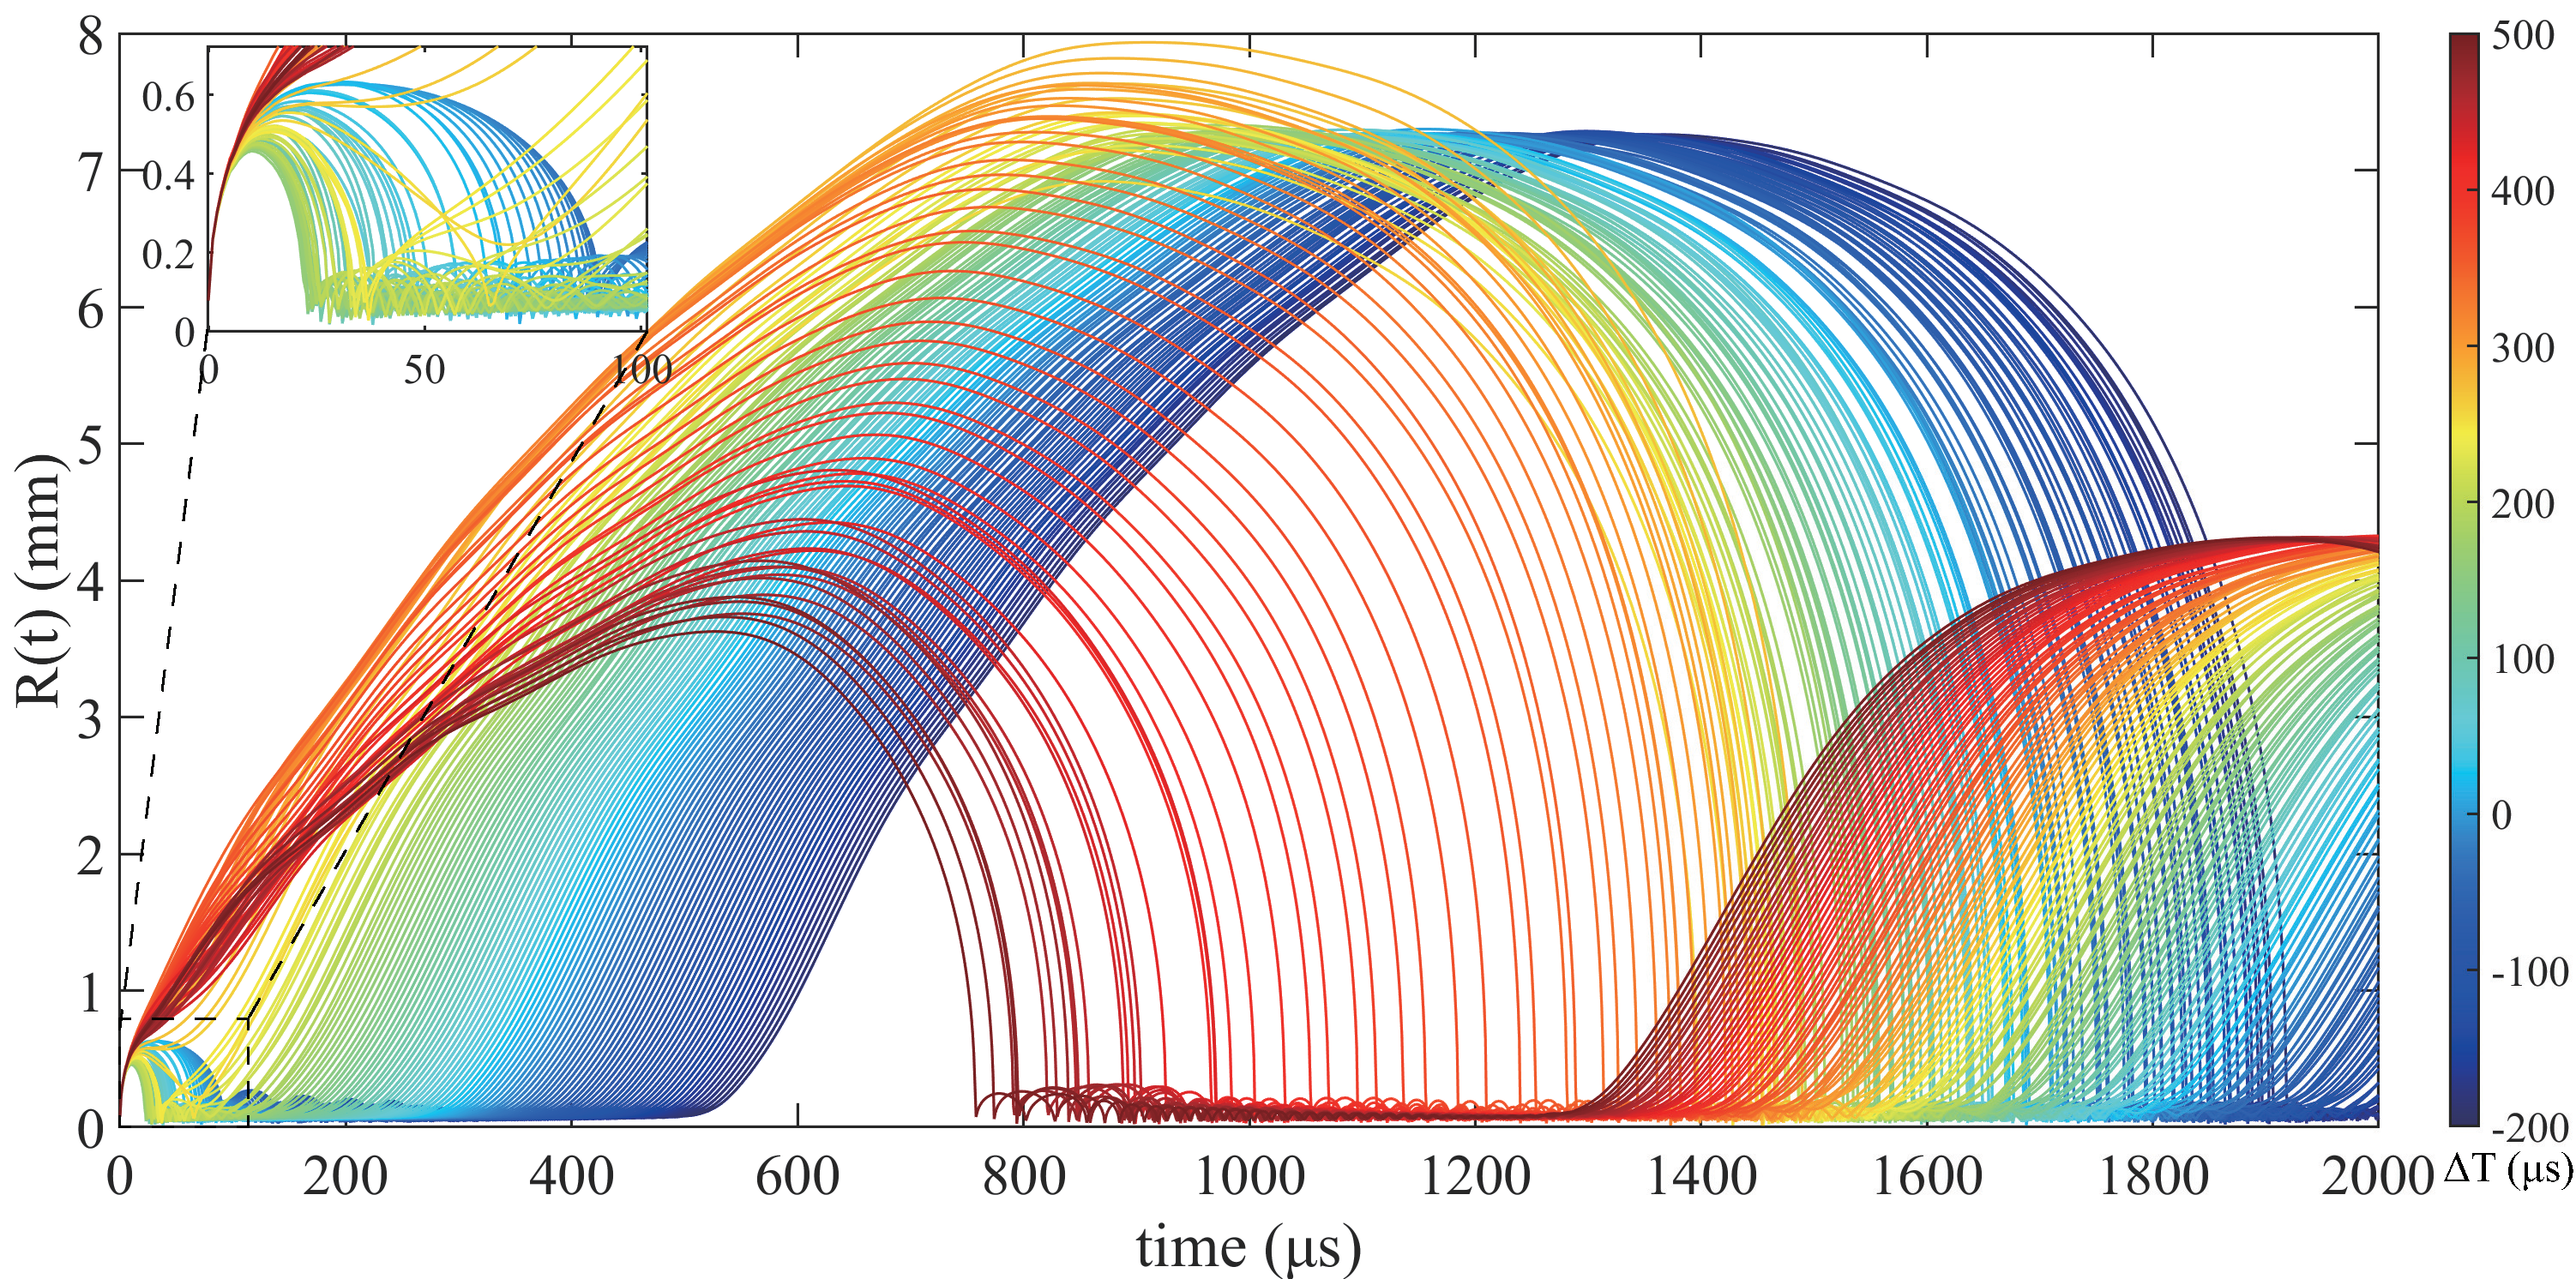
\includegraphics[width=1\linewidth]{img/fig5.16.pdf}
  \caption[使用 Keller-Miksis
模型与测量获得的压力波耦合计算的不同空泡诞生和压力波时延
$\Delta T$,情景下的空泡团簇脉动。]{使用 Keller-Miksis
模型与测量获得的压力波耦合计算的不同空泡诞生和压力波时延
$\Delta T$,情景下的空泡团簇脉动。在没有脉冲压力的情况下,空泡只在
100µs 左右扩展到大约 700µm(见∆T \textless{} -100µs
的曲线)。当空泡的引入在时间上与舒张波开始相吻合时,空泡膨胀获得最大半径,它在最大膨胀时可以达到
8 毫米以上。数值曲线高估了测量的空泡尺寸约 4
倍,我们将其归因于管壁的影响和由此产生的空泡的几何限制。}
  \label{fig:5.16}
\end{figure}




由张力波引起的空泡群或大体积空泡膨胀到最大半径,这是受管子的有限体积和张力波的双重影响。
K-M模型通常用来解释准自由域中的空泡行为,而在这项工作中,重生空泡的半径与管子半径相似,因此不是很准确。然而,我们发现计算和实验中的重生簇生存时间都在$1.3\,ms$左右。这是由管子的周围形状引起的,它延迟了膨胀和溃灭的过程。


\subsection{空泡溃灭致辐射冲击波}


与仅由恒定的环境压力驱动的溃灭相比,强制溃灭可能导致空泡的压缩增强。

在图 \ref{fig:5.17} 中,它显示了激光射入后不同 $\Delta T$ 情况下从 $0\,\mu s$
到 $200\,\mu s$
的压力云图。为了从数据中读取峰值压力,我们对记录的信号使用了 40 kHz
的高通滤波,以去除本底压力波。用箭头 A 标记的垂直高亮线,大约在
$7\,\mu s$
左右,是激光击穿冲击波在图中的表现。它到达水听器时,压力仍然很高,约为
3.5bar。

随后,在所有的情况下都存在这种崩溃冲击波的多次反射。箭头-B
指向第一个空泡崩溃冲击波的高亮带。在 $\Delta T<53\,\mu s$
的情况下,它位于 $104\,\mu s$ 左右。箭头 C
指向强制溃灭冲击波的高光曲线。由脉冲压力波引起的加速溃灭放大了溃灭冲击波。在高正压区,脉冲压力波和空泡残余物之间的进一步相互作用产生了许多后续的峰值,这主要是由容器的强化冲击波的反射引起的。在入射压力由正转负后,空泡在环境负压的作用下膨胀而没有溃灭,这被称为大空泡的产生,在上面的案例
c)中得到了说明。正如箭头-D 所指出的,在 $\Delta T=240\,\mu s$
之后,第一个空泡溃灭冲击波消失了。它合并到空泡团簇的溃灭冲击波中,这时被称为大空泡溃灭冲击波。

\begin{figure}[H]
  \centering
  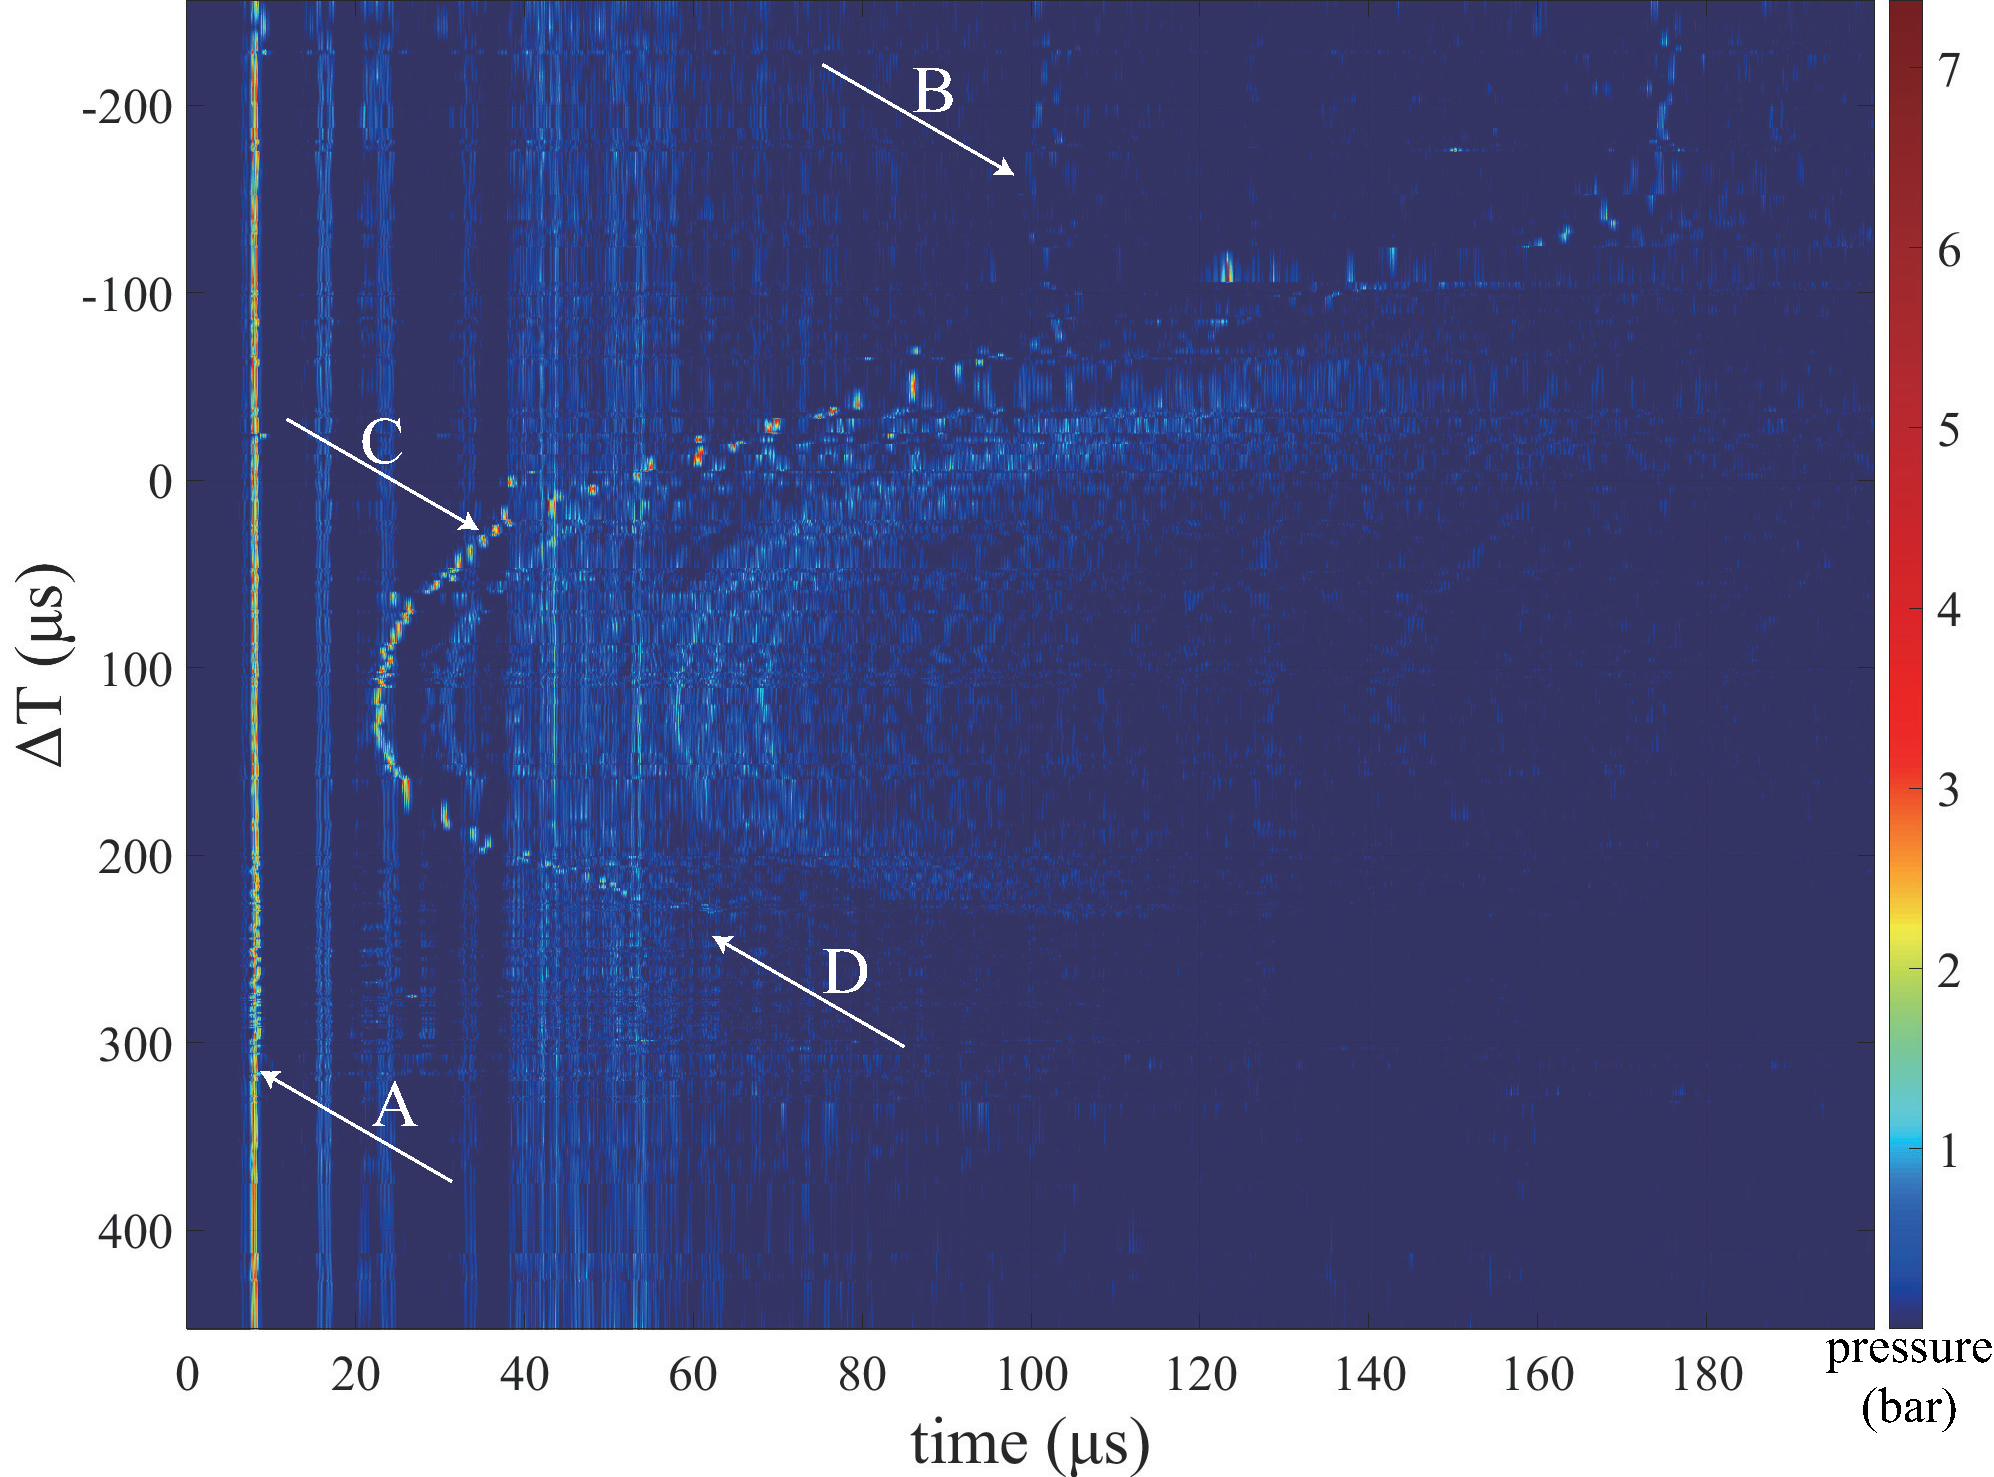
\includegraphics[width=0.8\linewidth]{img/fig5.17.pdf}
  \caption[10mm 处测得的压力云图]{10mm 处测得的压力云图。箭头
A:激光击穿冲击波。箭头-B:未受干扰的第一次空泡溃灭的溃灭冲击波,即当空泡在被脉冲压力波击中之前就已经溃灭。箭头
C 显示的是被脉冲压力波增强的第一次溃灭冲击波。对于较小的
$\Delta T$,表现为向左凹陷弯曲的曲线,因为压缩压力较早地击中了空泡,减少了空泡的生存时间。最终它又向右弯曲,因为空泡的大小在张力阶段变大。箭头-D:显示了第一次溃灭冲击波的消失,而实质上在该处空泡溃灭转变成大空泡机制,溃灭冲击波来自大的空泡溃灭。由于反射作用,A、C
所代表的冲击波的反射波在图中出现了多次。}
  \label{fig:5.17}
\end{figure}




为了表征溃灭强度,我们研究了不同 $\Delta T$
情况下的第一次溃灭冲击波峰值。图 \ref{fig:5.18} 中显示了(第一次)溃灭峰压力随
$\Delta T$
的变化。它包含了没有外界影响的空泡溃灭阶段、由压力波强迫的空泡溃灭,以及拉伸后的大空泡溃灭。每个溃灭峰值压力都经过了用其各自的等离子体冲击波峰值压力实施的归一化处理。即
$p=p_\text{impulse-peak}/p_\text{shockwave-peak}$。为了从数据中读取峰值压力,我们对记录的信号使用了
40 kHz 的高通滤波,以去除本底压力波。

空泡的生存时间显示为红色。空泡生存时间是击穿冲击波和溃灭冲击波两个峰值之间的时间差。蓝色曲线(第一次溃灭冲击波的峰值压力)的最大值在
$\Delta T\approx -30\,\mu$ s
附近。这一事实表明,当空泡在大部分时间在大气压力下膨胀,并且在空泡开始收缩时刻附近,瞬时压力波开始作用于空泡,此时空泡能够获得最强的溃灭增强(见图
\ref{fig:5.11} 中的波形)。

\begin{figure}[H]
  \centering
  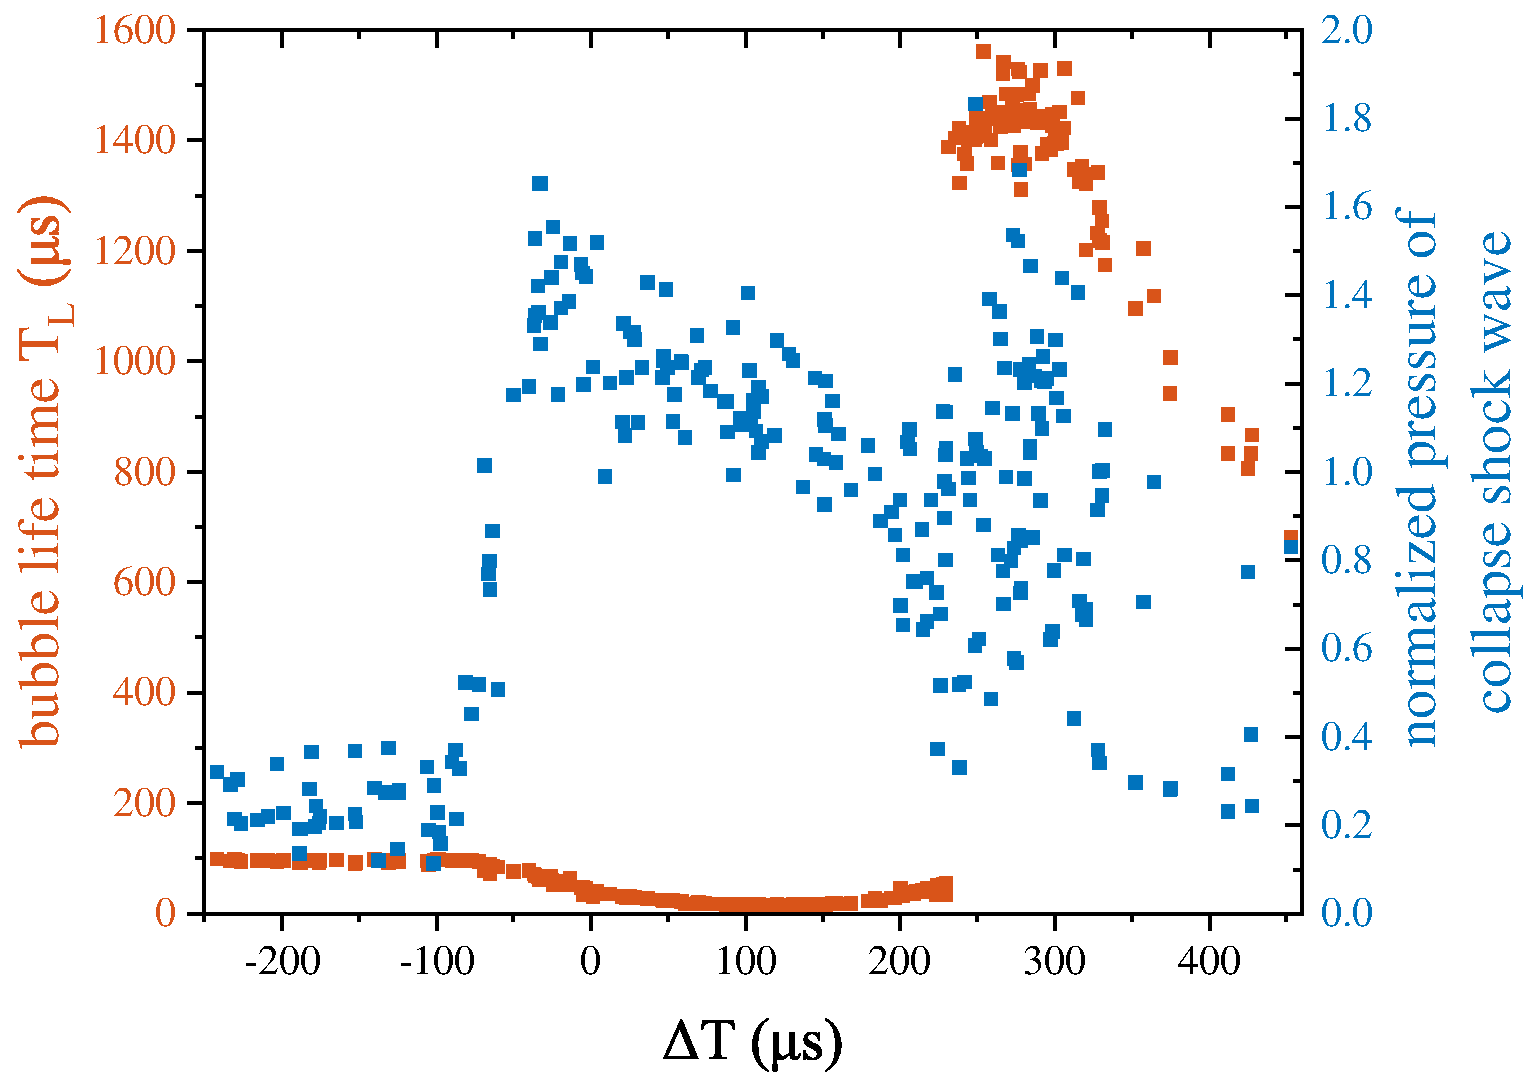
\includegraphics[width=1\linewidth]{img/fig5.18.pdf}
  \caption[第一个溃灭冲击波的峰值压力(蓝色)和空泡生存时间(红色)关于
$\Delta T$
的演化曲线]{第一个溃灭冲击波的峰值压力(蓝色)和空泡生存时间(红色)关于
$\Delta T$
的演化曲线。用到达监测水听器的冲击波时间减去等离子体的峰值时间,即空泡的生存时间。水听器测得该压力波峰除以测得的激光击穿冲击波获得其归一化压力。}
  \label{fig:5.18}
\end{figure}



作为对比,没有瞬时压力的静态空泡的溃灭峰值压力只有$\approx 0.2$,见$\Delta T<-100\mu$s,即第一次溃灭已经发生在脉冲压力波作用于空泡之前的情景。因此,可以认为溃灭增强在压力振幅方面约为$1.6/0.2=8$倍,在能量方面为$64$倍。
在这里,一个不同形状的波形,即有一个更陡峭的波前,可能会进一步改善崩溃的增强,我们预计在这种情况下,崩溃的最大峰值将转移到$T_\mathrm{L}/2$。

当$\Delta T$从这个最佳增强值增加时,由于空泡在压缩压力下已经膨胀并且其生存时间因此而减小,导致崩溃的峰值压力较小。在$\Delta T\approx230\,\mu$s之后,$T_\mathrm{L}$急剧增加到
$1\,$ms以上,这是因为如上文中所述的,溃灭阶段被稀疏波延长了。这导致溃灭峰值压力的测量有更多的变化,因为空泡在更长的时间内被膨胀到如此大的半径,不稳定因素导致主空泡破裂成通常两个较小的空泡,这些空泡的溃灭有时间偏移,产生两个振幅分别较小的溃灭峰值。然而,这种分裂过程有一些统计学成分,即空泡的大小可以在不同的运行中变化。

因此,一个与本文中的压力波反相的特殊构造的压力波,即具有领先稀疏和落后压缩相位,可以进一步改善溃灭增强。例如,这可以通过一个额外的反射器来实现瞬时压力的必要相移。



\section{空泡对压力波的特性的响应}

压力波通常指流体受到某种扰动,形成压力和密度等参数持续性波动并传播的现象。其包含多种情景,而正弦声波是其最简单的一种形式。
下面给出一个简单的一维小压力扰动即线性平面波传播的例子。考虑一个小尺度范围内的压力传播,如图
\ref{fig:5.19} 所示。该图右部表示常态,即未受扰动的状态,其压力密度和波速用下标 0
表示。扰动自左向右传播,其收到扰动的状态用下标 1
表示。波的传播仍遵从物质守恒和冲量守恒: $$
\left\{\begin{array}{lr}
\rho_1 u_1 A=\rho_0 u_0 A \\
(p_1-p_0)A=\rho_0 u_0 A(u_1-u_0)
\end{array}
\right.
$$

将式一所得 $u_1$ 代入式二可得: $
u_0^2=\frac {\rho_1} {\rho_0}(\frac{p_1-p_0}{\rho_1-\rho_0})
$

\begin{figure}[H]
  \centering
  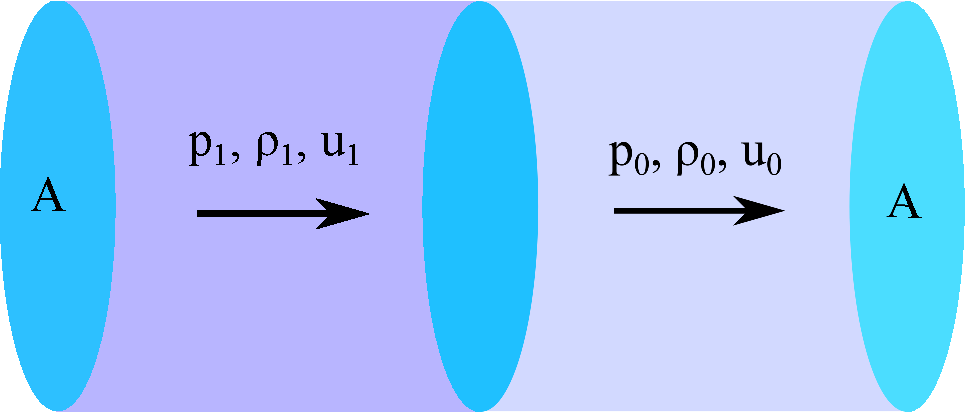
\includegraphics[width=0.5\linewidth]{img/fig5.19-eps-converted-to.pdf}
  \caption[压力波传播示意图]{压力波传播示意图。}
  \label{fig:5.19}
\end{figure}


若在低速低压域绝热系统内考虑,即在线性声波求解域内,前后密度差十分微小,即
$\rho_1 \approx \rho_0$,则有
$u_0=\sqrt {\frac {p_1-p_0}{\rho_1-\rho_0} }=\sqrt {\frac{\mathrm{d}p }{\mathrm{d}\rho}}\,.$
同时波的传播不代表其本地质点的速度
$u_\mathrm p$,通常平面波的压强与本地质点速度存在如下关系:
$p=\rho_0 u_0 u_\mathrm p\,.$ 注意,$\rho_1 \approx \rho_0$
有其适用条件,不同条件下可形成压缩波和膨胀波的演化,这里不做考虑。这里直接给出线性平面波的控制方程:
$
(\dfrac{\partial^2 }{\partial x^2}-\dfrac{1}{c^2}\dfrac{\partial^2 }{\partial t^2} )p =0
$ 此处 $c$ 是其本地声速。
本文只将包含膨胀和压缩波的压力波简单化为成正弦声波,而不考虑压力波的其他形式,即空泡中心和整体均遭受如下的时变声压:

\begin{equation}
\left\{\begin{array}{lr}
p =0\,&{t <\delta t_0},\\

p =A\mathrm {sin }(\dfrac{2\pi}{T_\mathrm {sine}}(t-\delta t_0))\,&{t \geq \delta t_0}。
\end{array}
\right.
\label{5.2.}
\end{equation}

其中 $\delta t$ 是声波入射时间,即
$t_\mathrm{pulse}$。在这个声波入射到空泡位置前,其声压为零,即只受液体的静压,这里采用的是
101325Pa。
为研究这个时变声压对空泡脉动的影响,设置了如下一个特殊空泡情景:
初始半径 $R_0=0.037\,\mathrm {mm}$,初始泡壁速度
$V_0=600\, \mathrm {m /s}$ , 均衡半径
$R_\mathrm n=0.075\,\mathrm {mm}$,最大泡半径
$R_\mathrm{max}=0.538\mathrm{mm}$, 第一脉动周期
$T_\mathrm {bubble }=100\,\mathrm\mu \mathrm s$ 。 由 Rayleigh-Plesset
(见第二章)的线性动力学形态,可以推导出空泡在零阻尼情况下的自然频率(谐振频率)\cite{brennen_cavitation_2003}: 
$$
\omega_\mathrm N=\left[\frac{1}{\rho_\mathrm{0} R_\mathrm{n}^2}\left\{3 \kappa (p_\mathrm{0}-p_\mathrm{v })+2(3 \kappa-1) \frac{\sigma}{R_\mathrm{n}}\right\}\right]^{\frac{1}{2}}
$$ 
各个字母含义均在第二章中给出,此处这个特殊的空泡情景有
$\omega_\mathrm N=2.28\times 10^5 \,\mathrm{Hz}$
,$T_\mathrm{N}=28\mathrm{\mu s}$。考虑到我们将主要关注空泡第一脉动周期,也就是受均衡半径
$R_\mathrm n$
影响较小的初期阶段,下文将主要从空泡第一脉动周期角度研究空泡诞生在这个压力波不同的相位对空泡自身脉动的影响。。


\subsection{压力波周期对空泡脉动的影响}

如本章实验所述,其压力波正压周期为 263.8
$\mu\mathrm {s}$,自由空泡的周期为 96 $\mathrm {\mu s}$ ,即
$\eta \approx 0.36$。本小节将主要针对压力波的周期与空泡周期的相对大小,即
$\eta$ 对空泡脉动的影响。影响主要体现在其实时半径和溃灭冲击波强度。
为一定程度上描述实验所述压力波对空泡行为的影响,在式 5.2.
X(此即时变声压)中,本节选择 $A=10\mathrm {bar}$。
为了获得溃灭产生的压力波强度 (collapse wave
pressure,CWP),假设空泡为完美球形脉动,将其看成一个振子,并基于不可压可获得下式\cite{Brennen2003}:

$$p_{\text{r}}(r,t)=\frac{\rho_{\text{L}}}{4\pi r}\frac{d^{2}V}{dt^{2}}$$
简化推导,不再赘述,可得:
$$p_{\text{r}}(R,r,t)=\frac{\rho_{\text{L}}}{r}\cdot R\cdot (2\dot R^{2}+R\ddot R)$$
上式由于基于不可压假设,其声压的传播是瞬时的,且其只包含几何衰减。获得特定位置的声压后,即可推得全场声压。本例中,采用
$r=10\mathrm{mm}$,即距空泡产生处 $10\mathrm{mm}$
($18.5R_\mathrm{max}$)
处的压力。此距离也与实验中,水听器的放置位置一致。考虑到在数值求解方程过程中,步长的选择将一定程度上影响解二阶导,即空泡壁面的加速度,使其不能准确命中突变。将解代入求解声压的过程中往往只能代表其大体趋势,而不是准确的描述其声压。参考声压级的获得方式,即先归一化再求其常用对数。本文中直接对求得的声压取常用对数,以减小突变和非突变解之间的差距。
\medskip
\bigskip
\subsubsection{
正弦周期小于空泡第一脉动周期}

首先考虑的一种情况,是式 5.2. X 的正弦周期小于空泡的第一脉动周期,即
$T_\mathrm{sine}<T_\mathrm {bubble }=100\,\mathrm\mu \mathrm s$,这里选择
$T_\mathrm{sine}=50 \mu s$,这样其正压的时长
$T_\mathrm{posip}=25\mu s$,则研究的相对时长参数
$\eta =0.25$。这种情况下,空泡在其孤立的自由地生存时间内,其能全面地遭受同时产生的压力的正压和负压。但在相互影响情景下,空泡将受正压压迫或负压拉伸。

\begin{figure}[H]
  \centering
  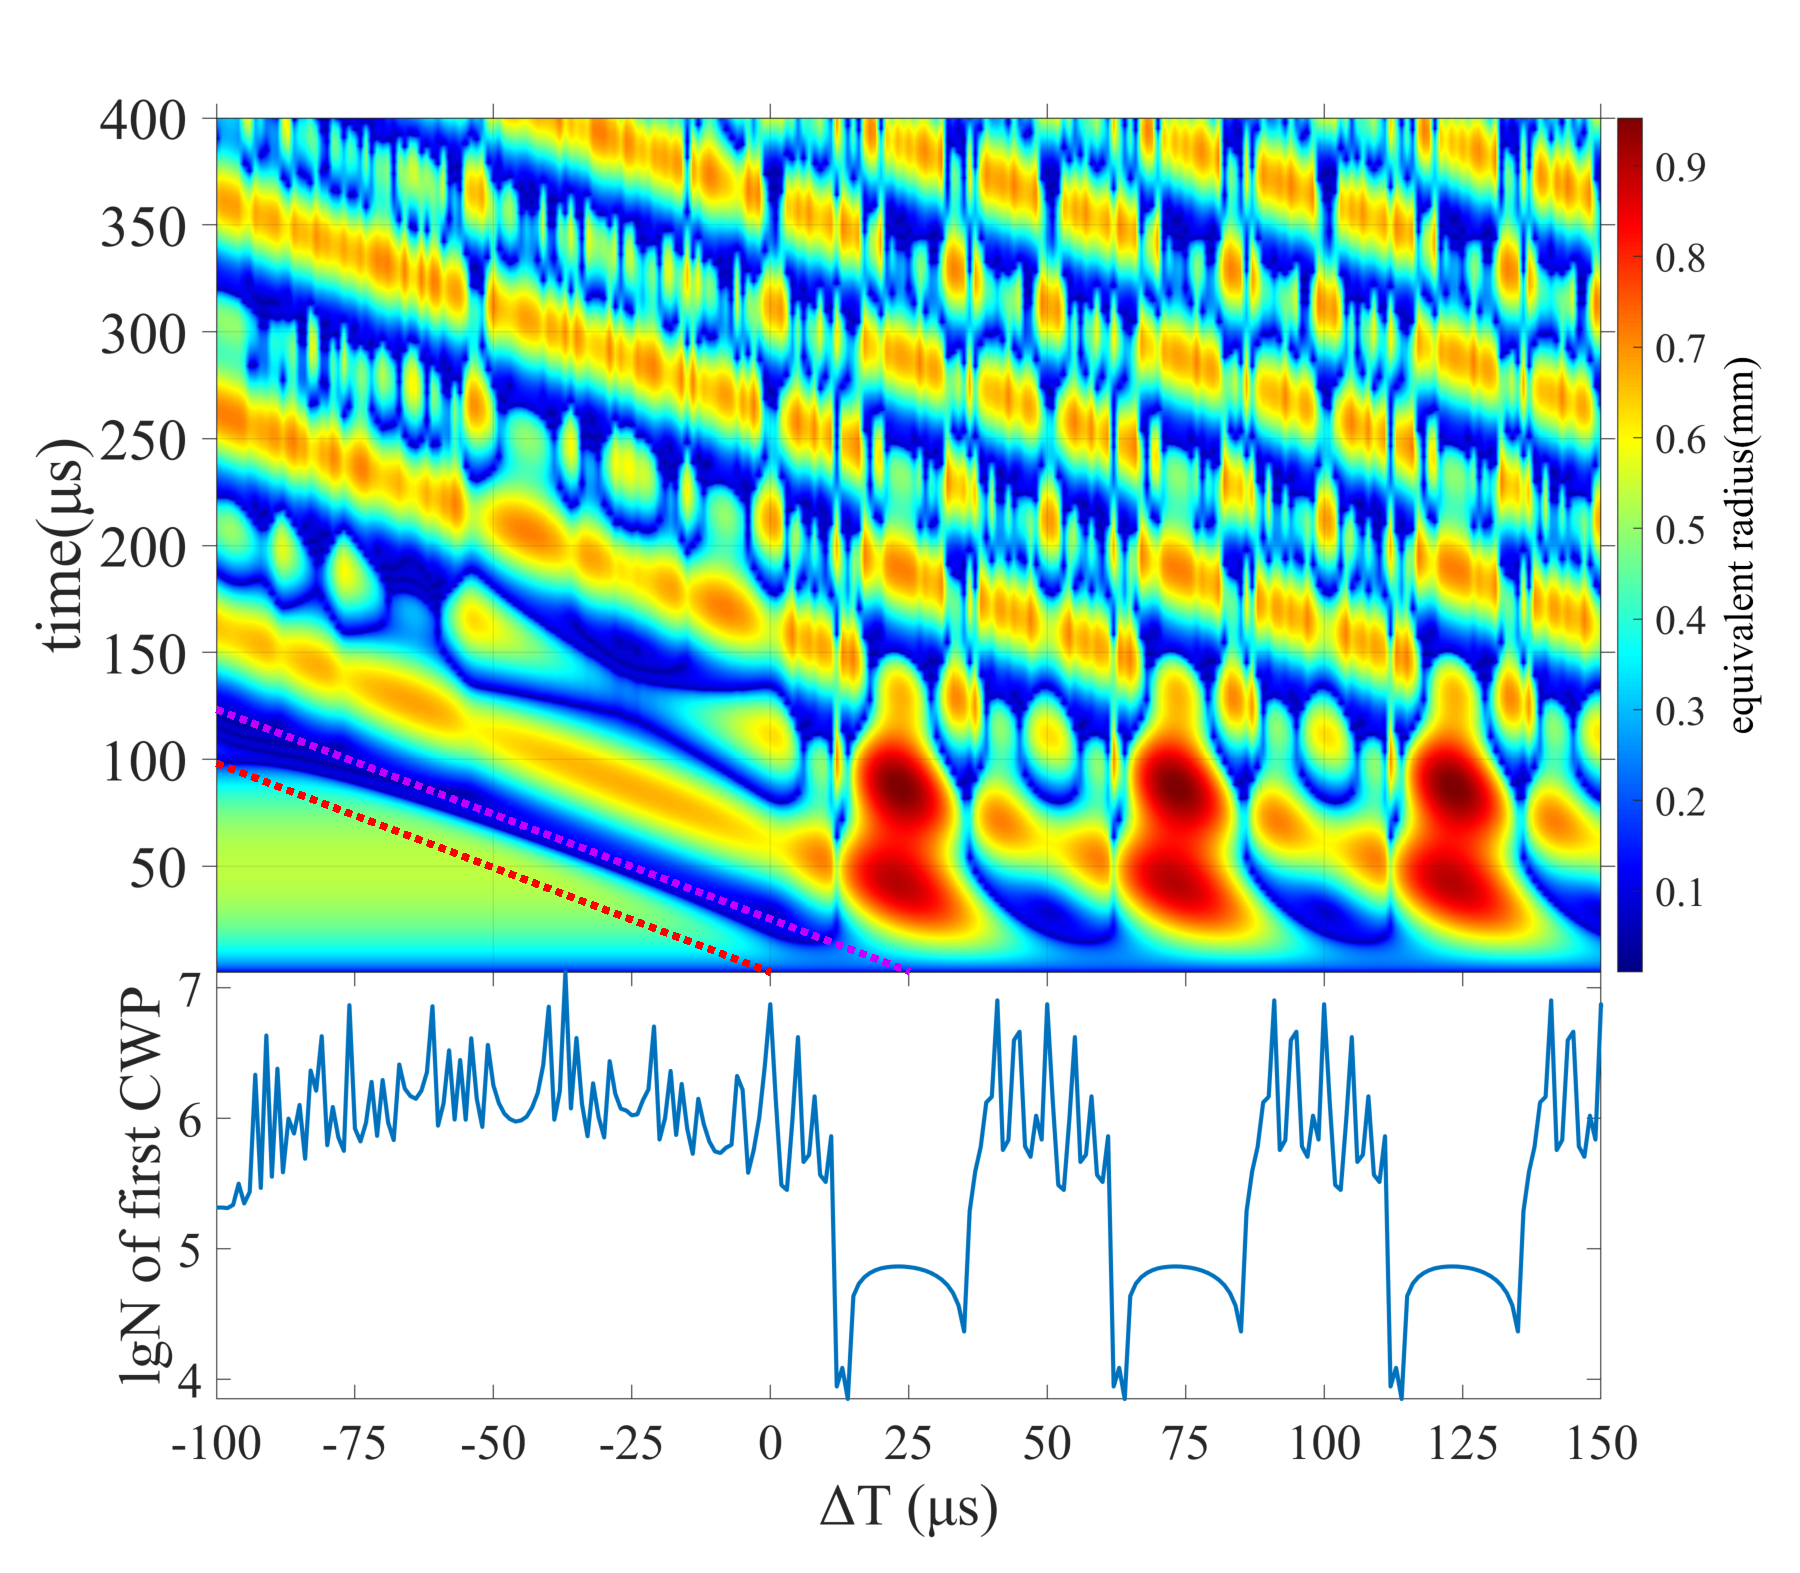
\includegraphics[width=0.9\linewidth]{img/fig5.20-eps-converted-to.pdf}
  \caption{$T_\mathrm{sine}=50 \mu s$
情景下,空泡受迫脉动的半径云图和空泡第一次溃灭产生的溃灭波压强(CWP)的对数级图。}
  \label{fig:5.20}
\end{figure}



图 \ref{fig:5.20} 上栏显示了
$-100\mathrm{\mu s}\leq\Delta T\leq150\mathrm{\mu s}$,即
$-1\leq\Delta \tilde{T} \leq1.5$
情境下,空泡半径随驱动压力波变动的云图。在
$-1\leq\Delta \tilde{T} \leq0$
时,空泡在受到正压后,受迫溃灭。其溃灭时间点连成的曲线是向外凸的,这与压力波的正弦波形有关,即其压强升高速度有关。它通过与空泡内压的相互作用的积分而使其空泡溃灭时间如图中变化。空泡溃灭后,其后续半径受压力波的正压阶段持续压缩,而形成空泡半径较小的蓝色条带。在受到负压作用后,空泡半径逐渐增长,并形成较孤立空泡最大半径大的半径。在这个范围的下栏,对应了空泡第一次溃灭的辐射声压。可以看到,其形成一个中间凸两边低的趋势,并在
$\Delta T=37\mathrm{\mu s}$ 处获得最大值。这也与实验中在
$\Delta T=30\,\mathrm{\mu s}$
处获得最大值的一致,即在空泡收缩阶段受正压加速溃灭速度形成更大溃灭辐射声压。在
$0\mathrm{\mu s}\leq\Delta T\leq10\mathrm{\mu s}$
,空泡诞生在压力波正压相内,其诞生后即收外界高压限制,不能足量膨胀。其溃灭声压也随其所受压力波正压积累而减小。在
$13\mathrm{\mu s}\leq\Delta T\leq35\mathrm{\mu s}$,空泡诞生后在溃灭前即遭受压力波的负压作用,或者空泡直接诞生在压力波的负压阶段。空泡在膨胀过程中遭受负压的拉伸作用,形成超量膨胀。而随即而来的正压对空泡的压缩加速作用,并不能使其在空泡超量膨胀的基础上溃灭,空泡的溃灭存在于第二个负压周期内。空泡在这种情况下,其半径会经历正压和负压作用而产生明显的波动,即膨胀后收缩,随即又膨胀。这个过程中,空泡消耗了压力波的驱动能量也释放了其自身动能。故而在第一次溃灭时形成的辐射声压显著减小。在
$35\mathrm{\mu s}\leq\Delta T\leq50\mathrm{\mu s}$
中,空泡诞生在负压相,受压力波的拉伸,并随后在压力波转到负压相后,受压力波的压缩此时亦呈现较高的溃灭速度,从而辐射较高的声压。在随后的
$\Delta T$ 中,空泡的脉动和辐射声压随压力波周期而周期性变化。
在空泡溃灭后并形成多次脉动的过程中,空泡受压力波驱动而逐渐形成受迫振动。形成类似于静态空泡受压力波驱动的形态,不在本作的关注点上,不再赘述。

\medskip
\bigskip
\subsubsection{正弦周期等于空泡第一脉动周期}

本节考虑 5.2. X 的正弦周期等于空泡第一脉动周期,即
$T_\mathrm{sine}=100 \mu s$,这时其正压时长
$T_\mathrm{posip}=50\mu s$,相对时长参数
$\eta =0.5$。在这种情况下,空泡在其孤立的自由地生存时间内,在膨胀期对应于同时产生的压力波的正压阶段,而在收缩期对应于该压力波的负压阶段,并在溃灭的时刻对应于负压到正压的转换。但在相互影响的情景下,空泡将受压力波影响,而减少或延长其生命周期。

\begin{figure}[H]
  \centering
  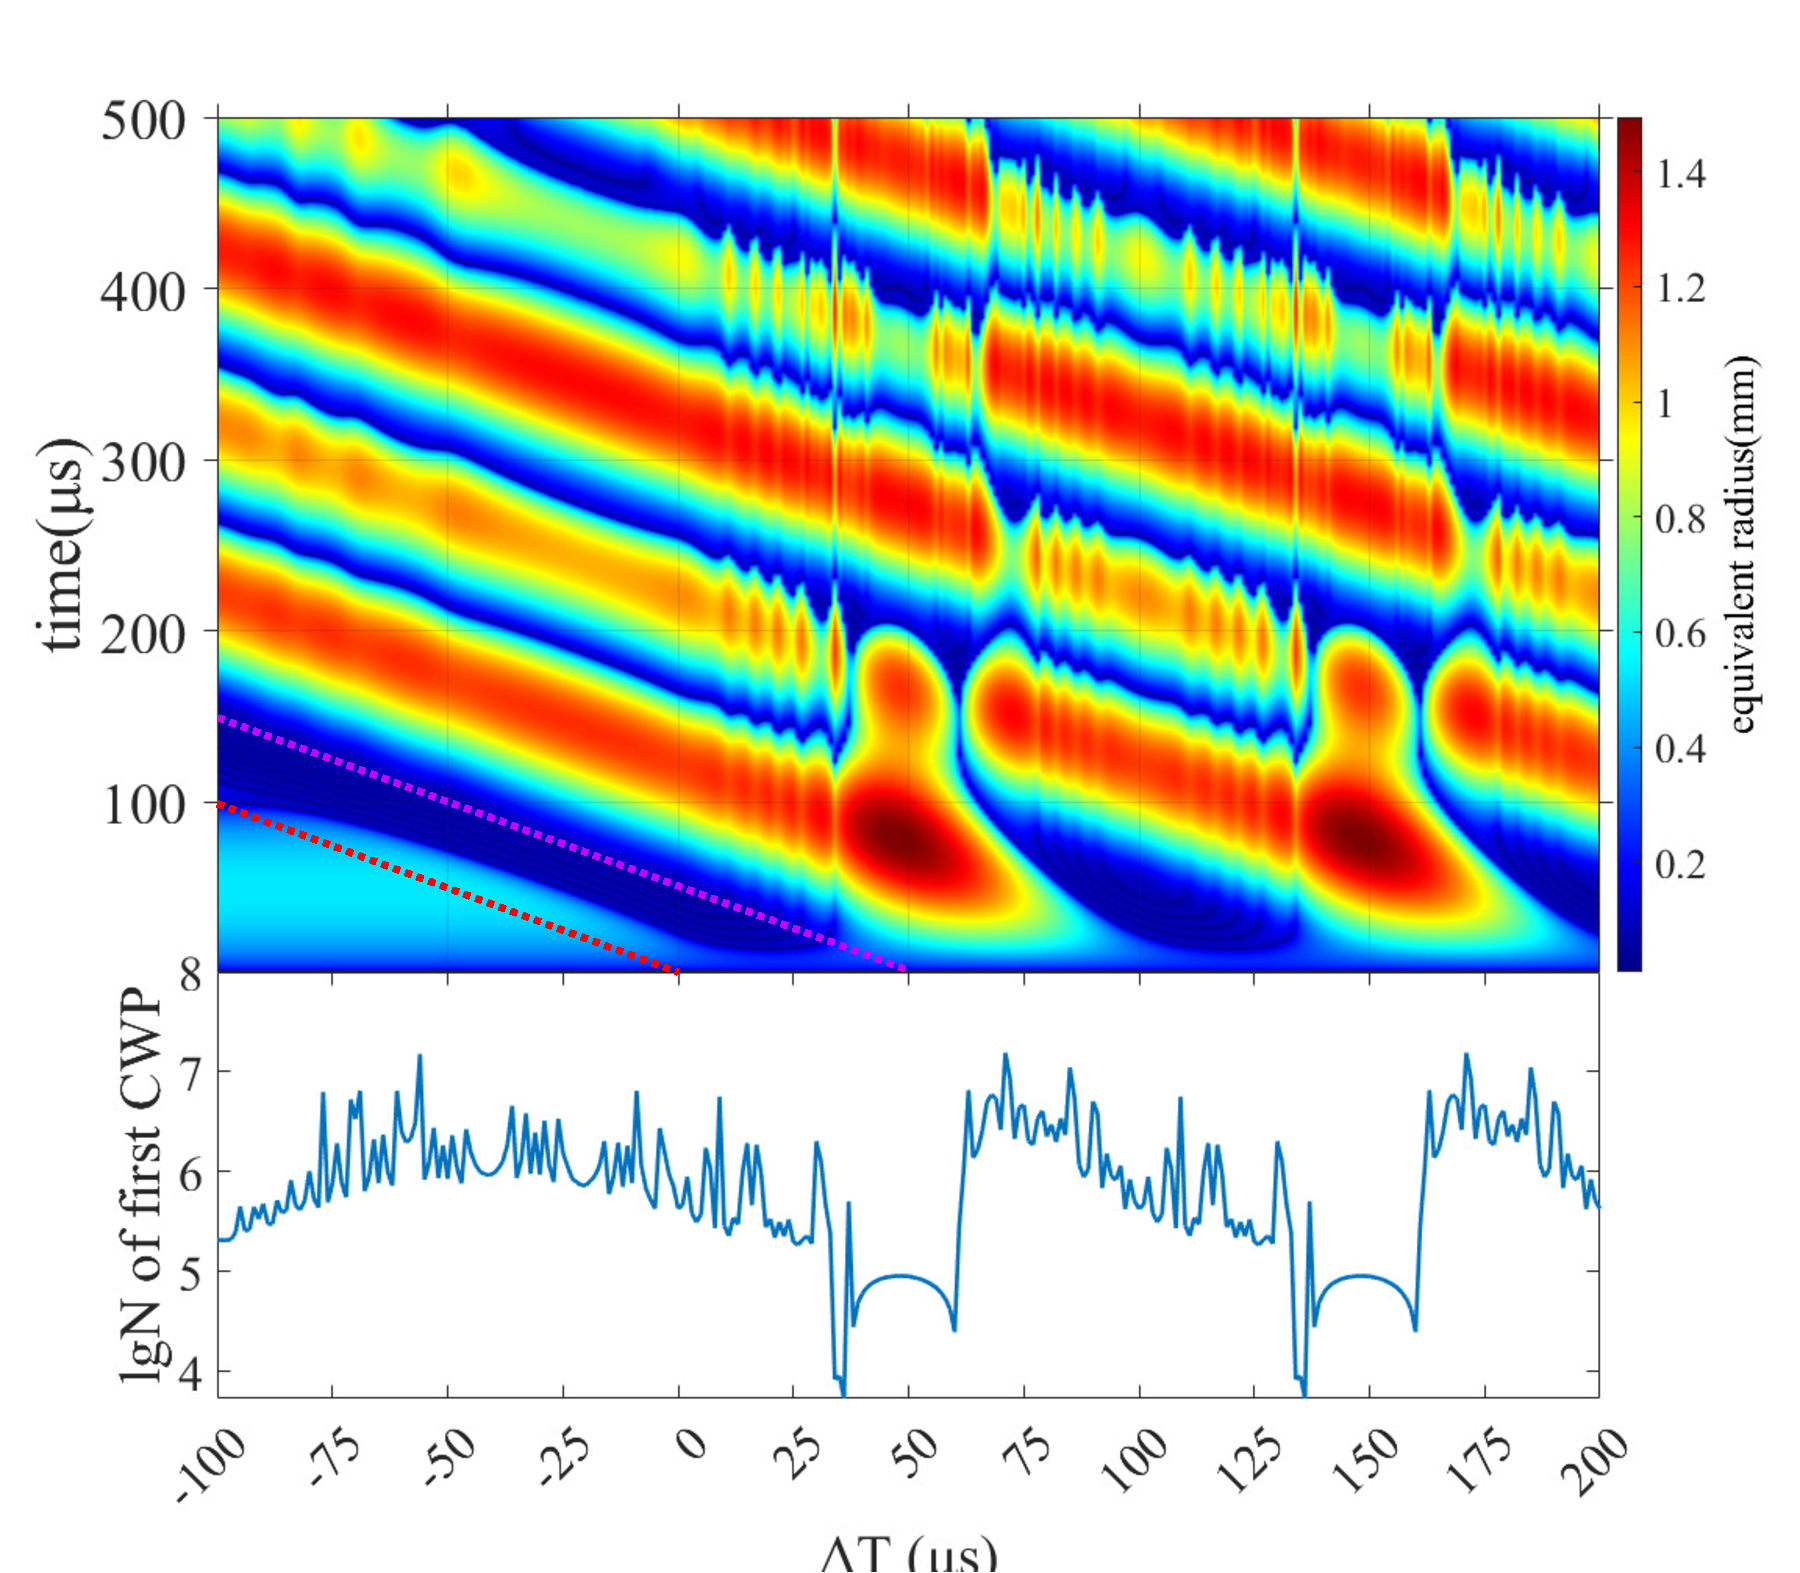
\includegraphics[width=0.9\linewidth]{img/fig5.21-eps-converted-to.pdf}
  \caption{$T_\mathrm{sine}=100 \mu s$
情景下,空泡受迫脉动的半径云图和空泡第一次溃灭产生的溃灭波压强(CWP)的对数级图。}
  \label{fig:5.21}
\end{figure}


图 \ref{fig:5.21} 显示了 $-100\mathrm{\mu s}\leq\Delta T\leq200\mathrm{\mu s}$,
即 $-1\leq\Delta \tilde{T} \leq2$
情境下,空泡半径随驱动压力波变动的云图,和空泡第一次溃灭辐射声压曲线图。与图
\ref{fig:5.20} 类似,图 \ref{fig:5.21} 
也表现出了压力波强迫溃灭和舒张波阻止溃灭并强制拉伸的作用。与图 \ref{fig:5.20} 
不同的是图 \ref{fig:5.21} 
中由于压力波周期更长,空泡在受拉伸超量膨胀过程中,空泡并不能保持相对更长的时间。表现在图中就是在
$\Delta T=45\,\mathrm{\mu s}$
附近,空泡的第一次溃灭前只有两个极值峰,对应的图\ref{fig:5.20} 中
$\Delta T=25\,\mathrm{\mu s}$
附近则有三个峰。而在辐射声波图中则可以看到在
$\Delta T=37\,\mathrm{\mu s}$
附近,此时空泡在第一次溃灭前只有一个半径最值峰,图中捕捉到一个辐射压力峰。这个峰是发生在空泡由小空泡溃灭到大空泡溃灭形式转变的节点后的。
与上一小节类似,溃灭辐射声压在空泡受迫溃灭阶段形成加强,其加强效果随
$\tilde{T}$ 在 $(-0.5, \,0.4)$
范围内增长而减小。而因负压拉伸并受正压强迫溃灭的阶段,即空泡在溃灭前只经历一个半径最值峰,也就是
$\Delta \tilde{T}\in (0.65,\,1.3)$ ($\Delta T \in (65,\,130)$
),效果更加明显的呈下降趋势。

\medskip
\bigskip
\subsubsection{正弦正压相周期等于空泡第一脉动周期}

本节考虑 5.2. X 的正弦周期等于二倍的空泡第一脉动周期,即
$T_\mathrm{sine}=200 \mu s$,这时其正压相周期等于空泡第一脉动周期
$T_\mathrm{posip}=100\mu s$,相对时长参数
$\eta =1.0$。在这种情况下,空泡在其孤立的自由地生存时间内,其整个生存寿命对应于同时产生的压力波将都在压力波的正压阶段。在相互影响的情景下,空泡将更加明显的受压力波单相位的影响。

\begin{figure}[H]
  \centering
  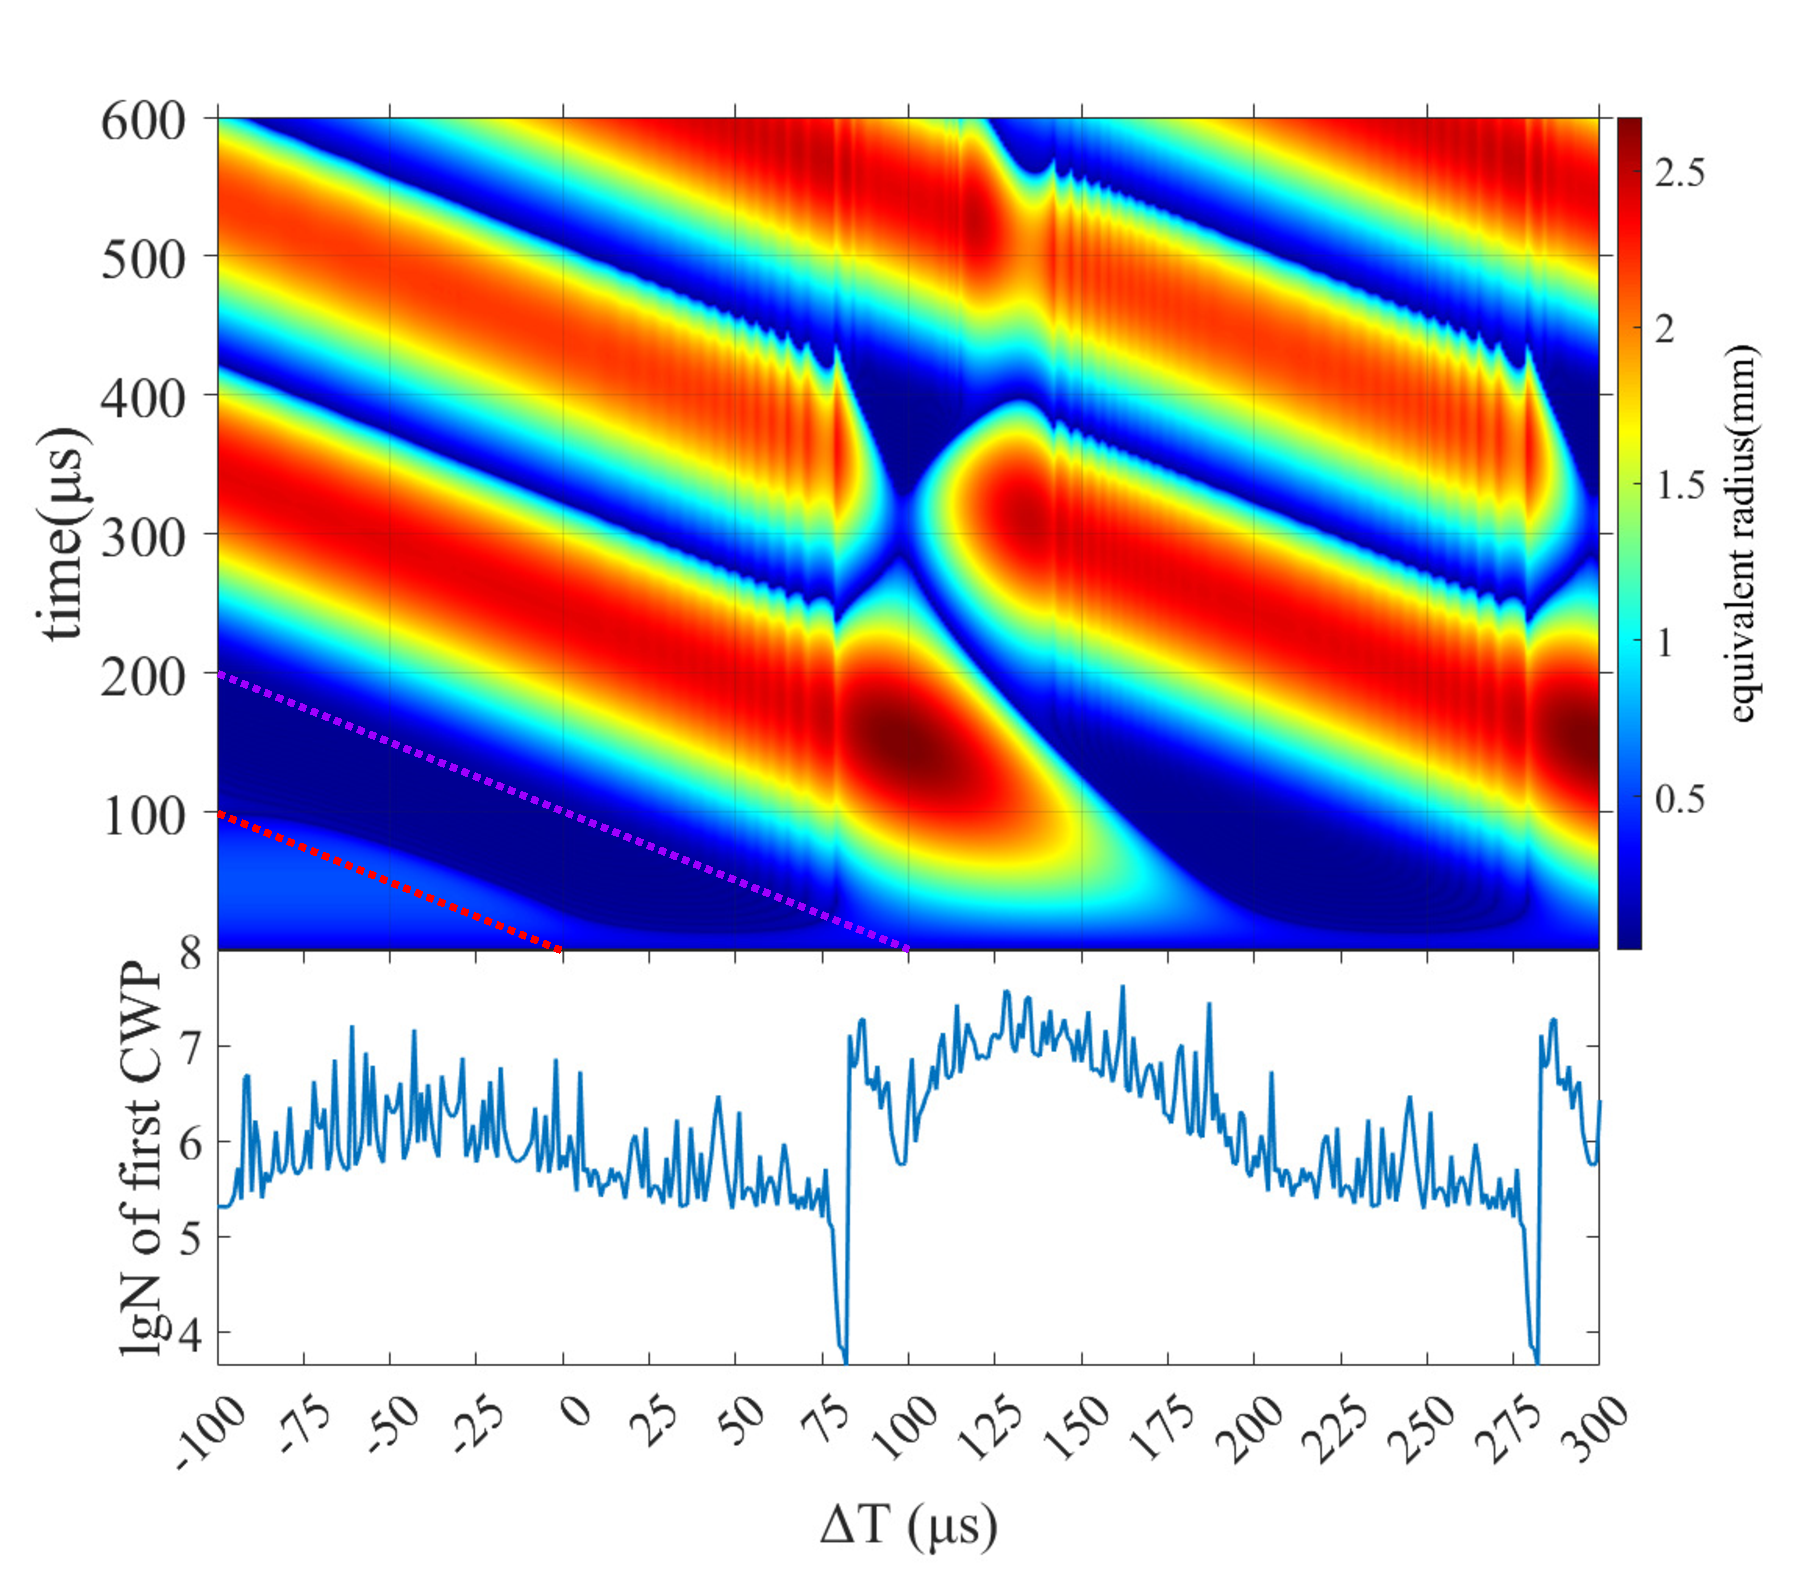
\includegraphics[width=0.9\linewidth]{img/fig5.22-eps-converted-to.pdf}
  \caption{$T_\mathrm{sine}=200 \mu s$
情景下,空泡受迫脉动的半径云图和空泡第一次溃灭产生的溃灭波压强(CWP)的对数级图。}
  \label{fig:5.22}
\end{figure}


图 \ref{fig:5.22} 显示了 $-100\mathrm{\mu s}\leq\Delta T\leq300\mathrm{\mu s}$,
即 $-1\leq\Delta \tilde{T} \leq3$
情境下,空泡半径随驱动压力波变动的云图,和空泡第一次溃灭辐射声压曲线图。此情景获得结果类似于实验结果,图
\ref{fig:5.15} 。在空泡半径最大值附近入射正压获得辐射声压的最值,并随 $\Delta T$
增长而减小。并如同图 \ref{fig:5.20} 和图 \ref{fig:5.21} 
一样存在一个下降的突变。溃灭冲击波的减弱区的减小的十分明显,这是因为本例中空泡没有单脉动周期多半径极值的情况存在。特别的是在
$\Delta T=100\mathrm{\mu s}$
,即空泡诞生于压力波由正转负的节点处的空泡脉动的特别突出部。空泡的响应压力波的第一次脉动周期在
$\Delta T\in (80,100)\mathrm{\mu s}$
内呈现递增趋势。并且在辐射声压在区间前的突变后,该辐射声压逐渐减少。而在
$\Delta T=125\mathrm{\mu s}$
处获得最大辐射声压,此时空泡溃灭恰好在驱动压力波由正压转换为负压的节点。在
$\Delta T=(100,125)\mathrm{\mu s}$
区间,空泡因受负压作用而超量膨胀,其溃灭发生在另一个负压相内,所以溃灭辐射声压较
$\Delta T=125\mathrm{\mu s}$ 处小。而随着 $\Delta T$
在区间内增长,空泡受另一个负压相作用的时间越短,其辐射声压就越大。而在
$\Delta T=(125,200)\mathrm{\mu s}$
区间内空泡遭遇压力波负压相后又遭受正压相,其溃灭辐射声压因此加强,并随
$\Delta T$ 增长,空泡第一脉动周期减小而减小。

\medskip
\bigskip
\subsubsection{正弦正压相大于空泡第一脉动周期}


\begin{figure}[H]
  \centering
  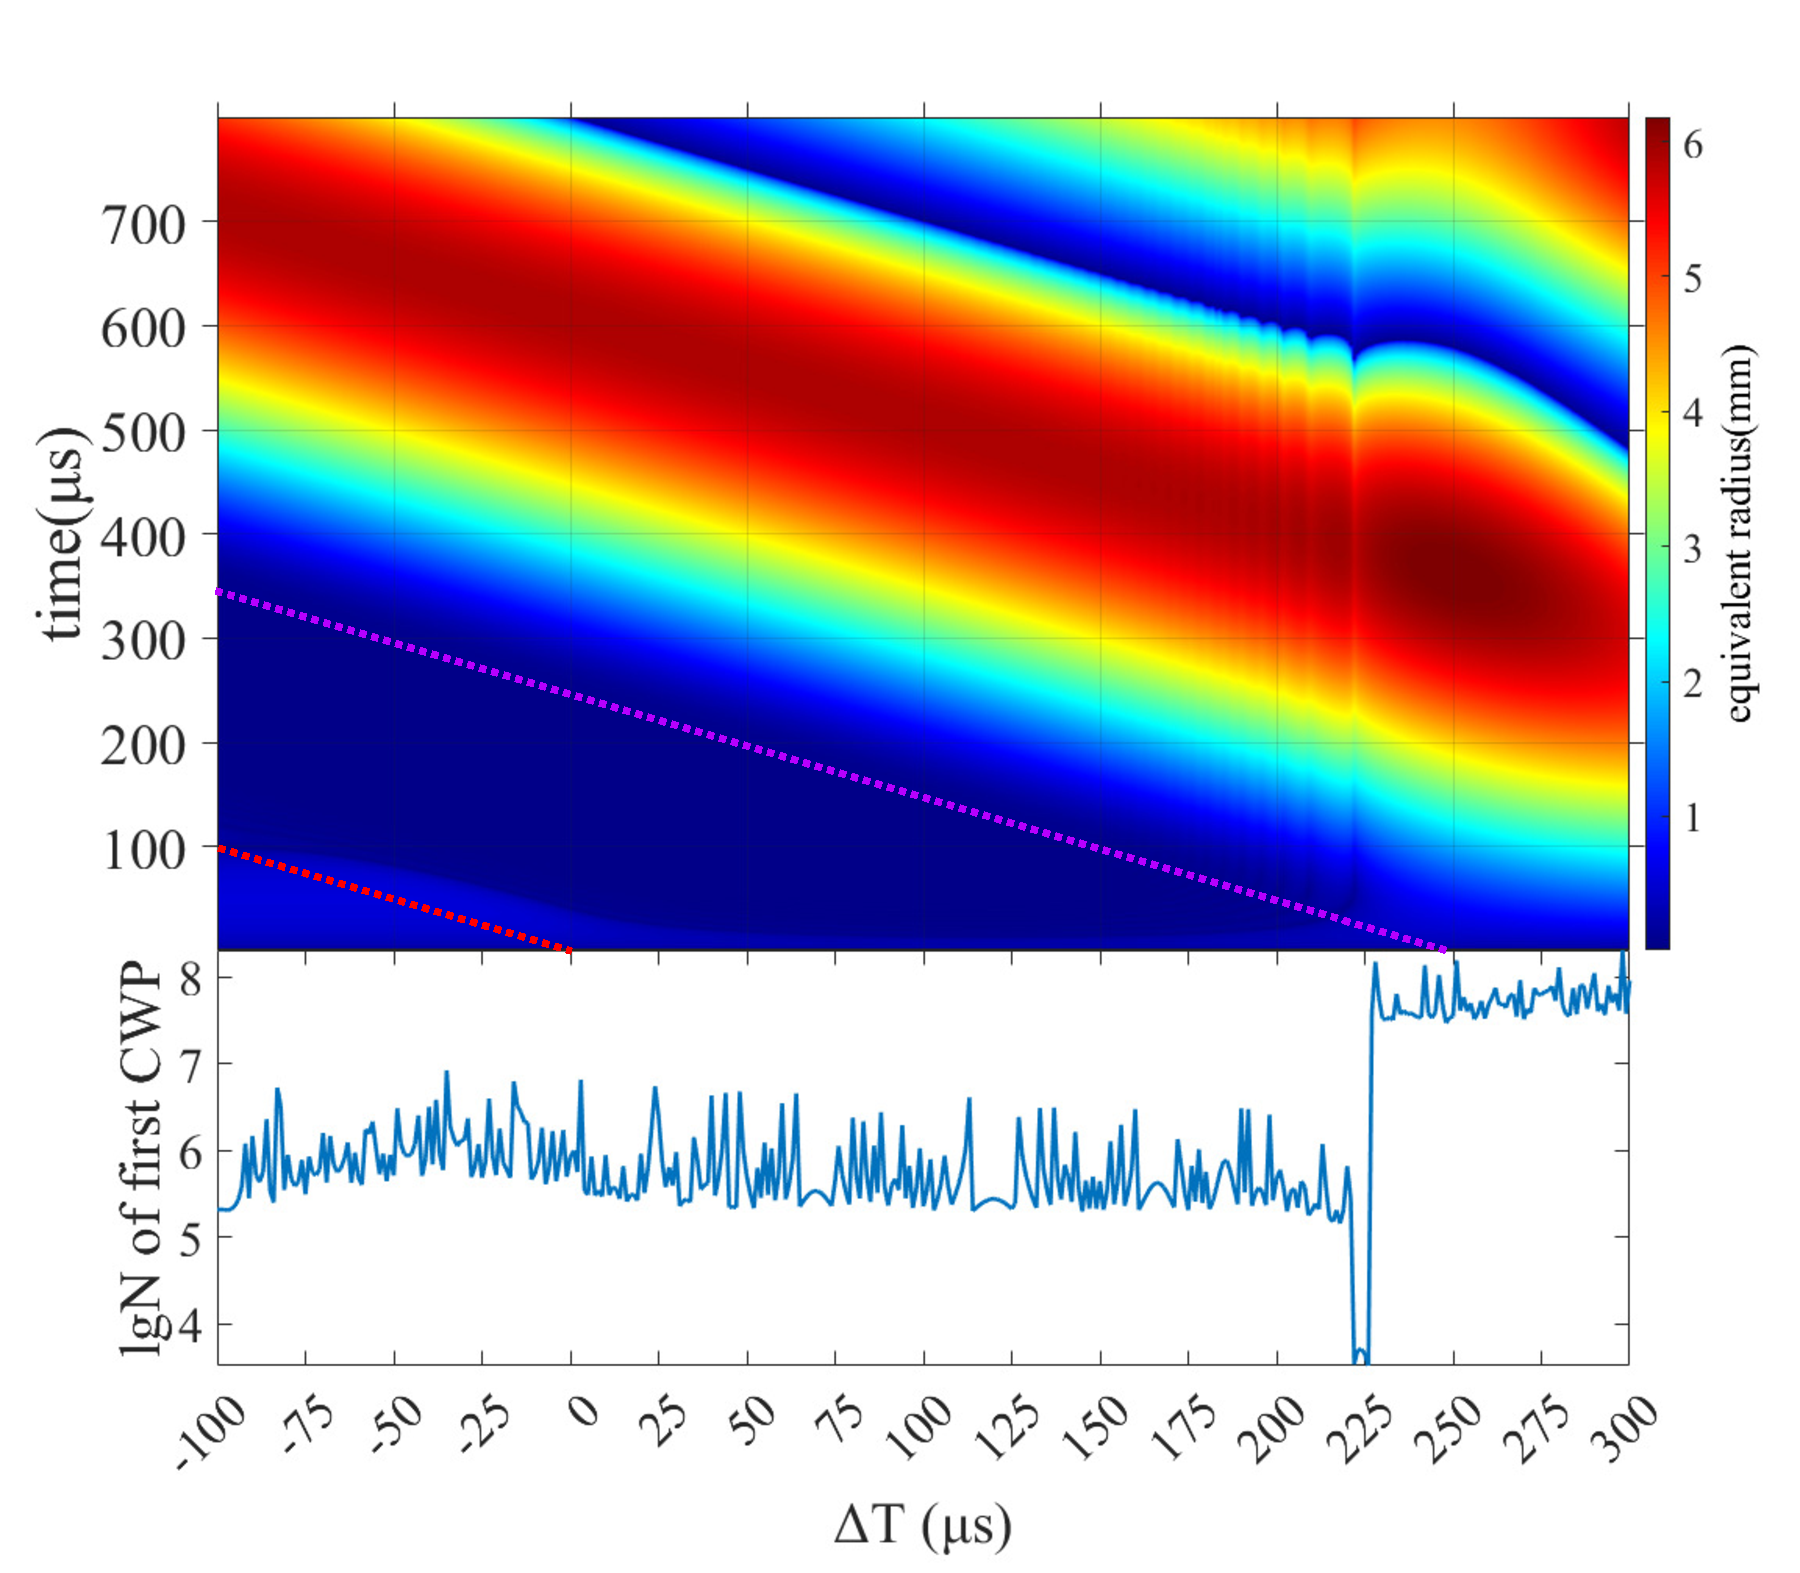
\includegraphics[width=0.9\linewidth]{img/fig5.23-eps-converted-to.pdf}
  \caption{$T_\mathrm{sine}=500 \mu s$
情景下,空泡受迫脉动的半径云图和空泡第一次溃灭产生的溃灭波压强(CWP)的对数级图。}
  \label{fig:5.23}
\end{figure}

本节考虑 5.2. X 的正弦正压相周期大于空泡第一脉动周期,即
$T_\mathrm{posip}>T_\mathrm {bubble }=100\,\mathrm\mu \mathrm s$,,这里选择
$T_\mathrm{sine}=500 \mu s$,
$T_\mathrm{posip}=250\mu s$,相对时长参数
$\eta =2.5$。在这种情况下,空泡在其孤立的自由地生存时间内,其整个生存寿命对应于同时产生的压力波将都更加明显的在压力波的正压阶段。在相互影响的情景下,空泡受压力波影响形成的改变将更加突出。



图 \ref{fig:5.23} 显示了 $-100\mathrm{\mu s}\leq\Delta T\leq300\mathrm{\mu s}$,
即 $-1\leq\Delta \tilde{T} \leq3$
情境下,空泡半径随驱动压力波变动的云图,和空泡第一次溃灭辐射声压曲线图。此情景下空泡的最大泡半径可以达到十倍于
$R_0$,但脉动周期对压力波周期的跟随性更加突出。特别地,本例中,溃灭辐射声压的加强情况非常明显,这是由于空泡诞生在负压阶段的超量膨胀现象特别明显导致的。

\medskip
\bigskip
\subsubsection{
溃灭致冲击波}

上文四个小节中,分析了四例不同周期的压力波与空泡相互作用对空泡半径和溃灭辐射声压的影响。其中溃灭辐射声压值得更全面的视角分析。

\begin{figure}[H]
  \centering
  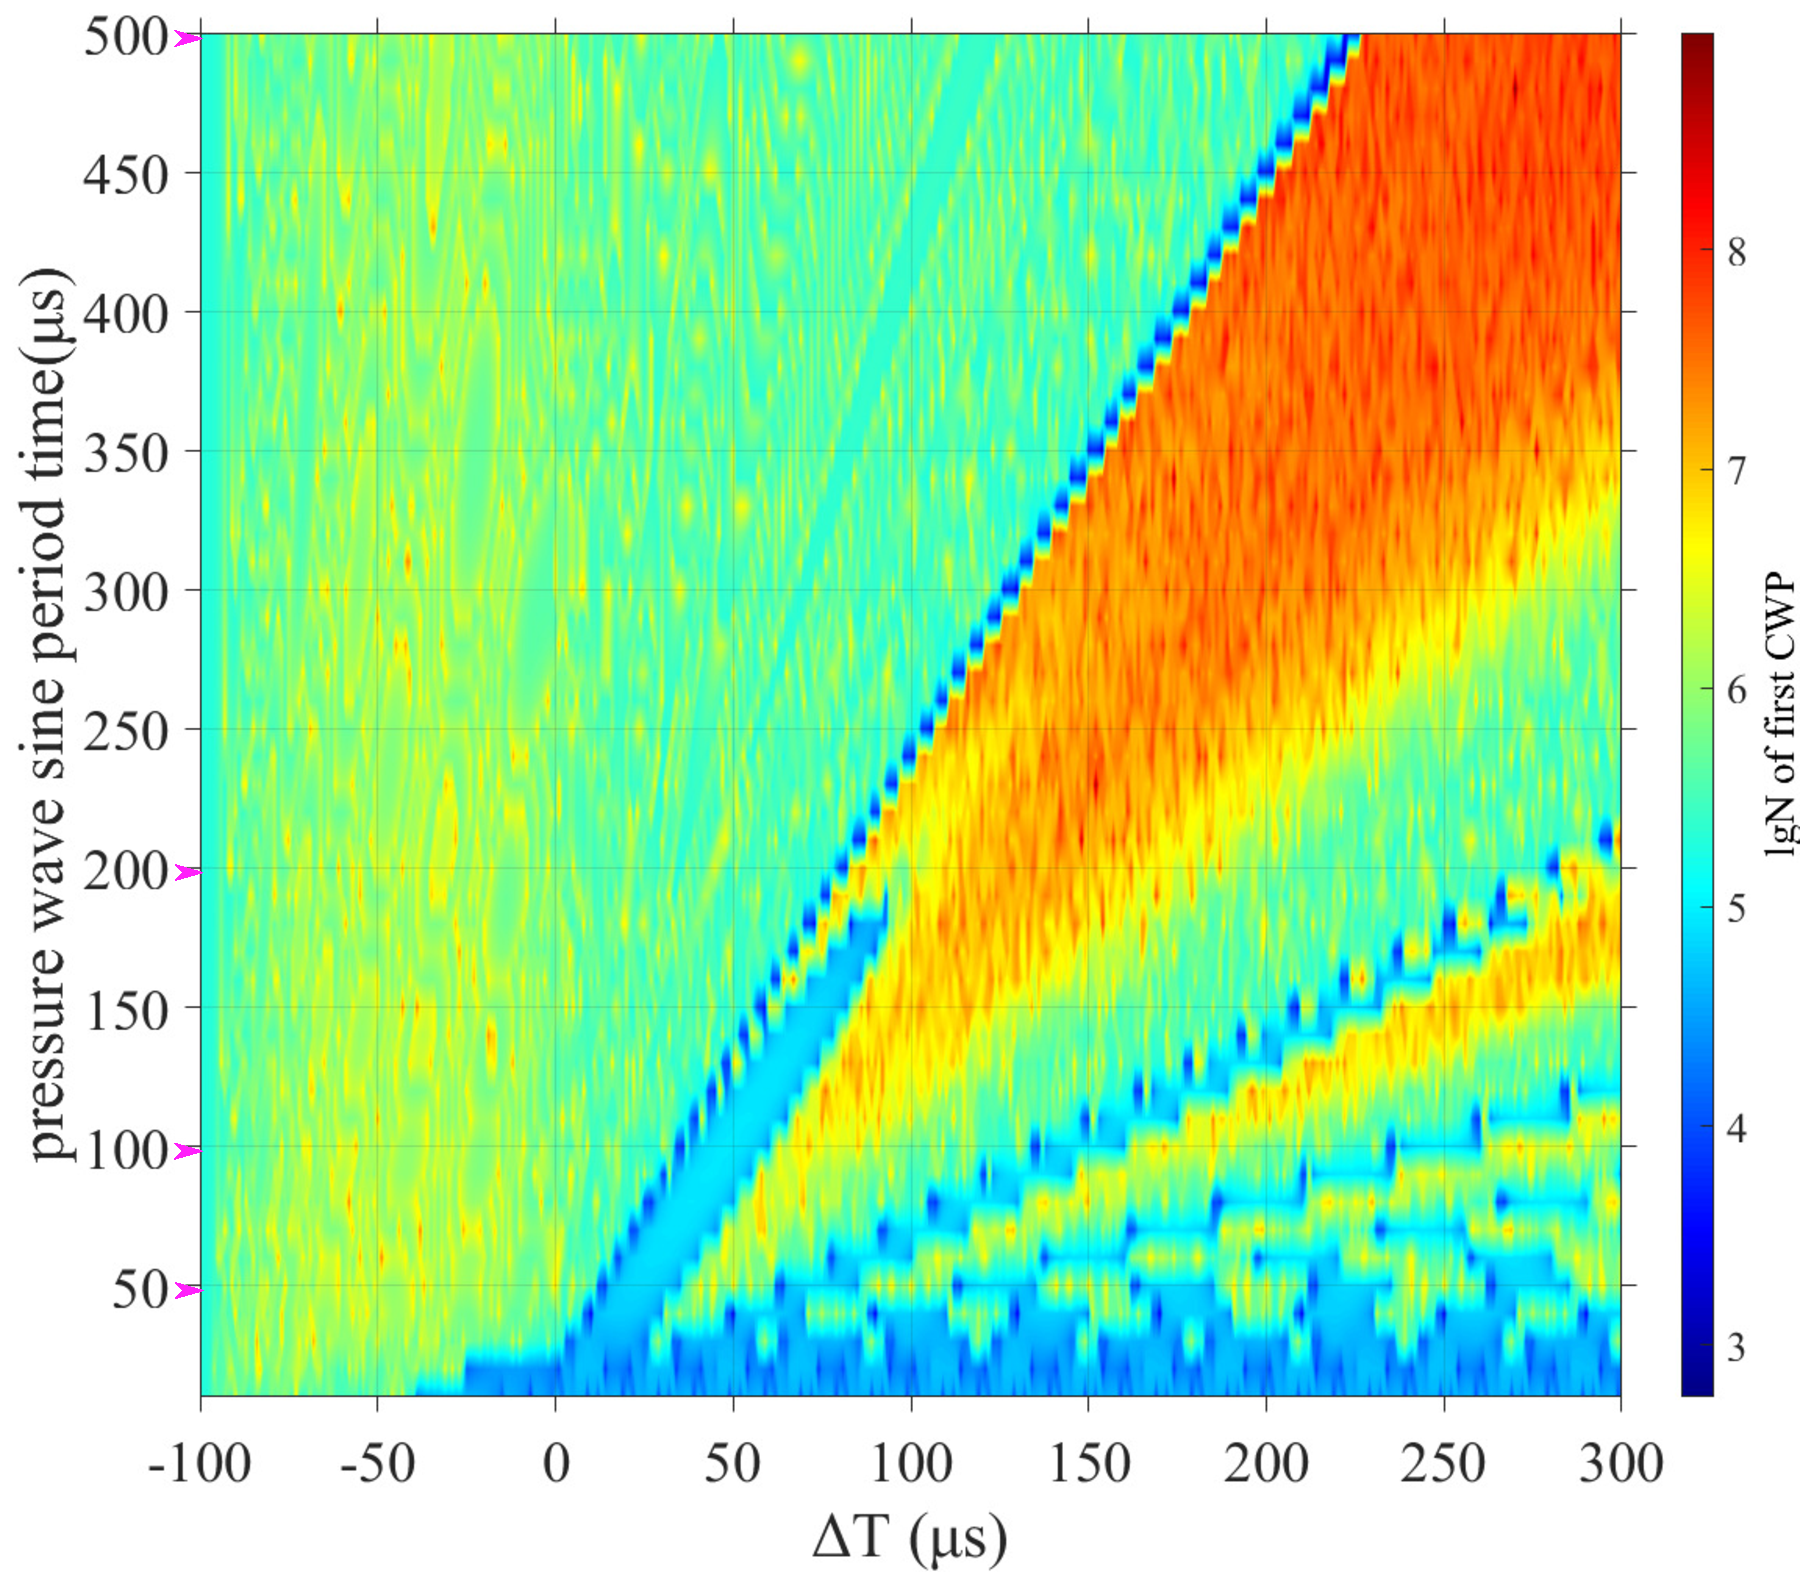
\includegraphics[width=0.9\linewidth]{img/fig5.24-eps-converted-to.pdf}
  \caption{在振幅为 10bar
情况下的,压力波周期和 $\Delta T$ 影响下的空泡溃灭压力波压强云图。}
  \label{fig:5.24}
\end{figure}

如图 \ref{fig:5.24} 显示的溃灭辐射声压基于压力波周期和参考时延 $\Delta T$
的云图。可以看到在 $\Delta T<0$ 时,其在 $\Delta T=50\mathrm{\mu s}$
附近有一个高峰,这代表的空泡在产生后受正压作用会产生溃灭增强。而在
$\Delta T=0\mathrm{\mu s}$
后,有一片没有声压增强的区域。这里显示的是空泡诞生在压力波正压相内时其增强很小,甚至在某些区域会有减弱效果,如淡蓝色三角带显示。图中非常明显的存在一条蓝色线性区域,它代表着空泡的溃灭方式由正压强迫溃灭的小空泡到负压拉伸至超量膨胀状态的大空泡的溃灭附近存在的一个特殊状态,也是在压力波由正压相到负压相转变前的一个特殊时刻,是空泡在受正压压迫而极速收缩,但溃灭时其环境压强已经转换为负压相,从而形成小空泡慢速溃灭,由此而表现出这样一条弱辐射声压线性条带。
在 $T_\mathrm{sine}<200\mathrm{\mu s}$
的蓝色条带后,可以看到存在着一片声辐射减弱区域。这里对应的是空泡受高频(短周期)压力波影响,形成的在空泡第一个脉动周期内存在多个半径极值峰的现象,并辐射较小声压的域。在这个区域中,空泡受舒张波影响,达成第一阶段的超量膨胀,但正压作用后并没有能及时的阻止其继续膨胀,空泡在正压阶段受正压驱动溃灭的过程就因此减少了作用时间,并使其不能做完全的加速溃灭,甚至使空泡在下一个负压相溃灭,使空泡因收缩速度减慢而形成较弱的声压辐射。在这个状态下,空泡的能量和压力波的能量主要耗散在空泡的受迫阻尼振动中。这里也能够解释在上一节实验中的
$\Delta T=238\mathrm{\mu s}$
左右处形成了一个低声压极值谷。更特殊的是在更高频低周期($T_\mathrm{sine}<20\mathrm{\mu s}$
)压力波作用下存在的空泡,其辐射声波普遍较小。
更普遍的,在蓝色的减弱区间结束后,随之而来的是在低频(长周期)外压的驱动下,一片较为广大的空泡溃灭辐射声压加强区域。其边界也较为清晰,呈线性排布。这个区域的形成代表空泡膨胀期受负压作用形成超量膨胀,而后在正压作用下受迫溃灭,也就是大空泡快速溃灭,从而辐射更高的声压。这也验证了上一节中最后一段所预测的,可以通过构造特殊的压力波从而在应用环境中形成加速空泡溃灭冲击的效果。


\subsection{压力波振幅对空泡脉动的影响}

\begin{figure}[H]
  \centering
  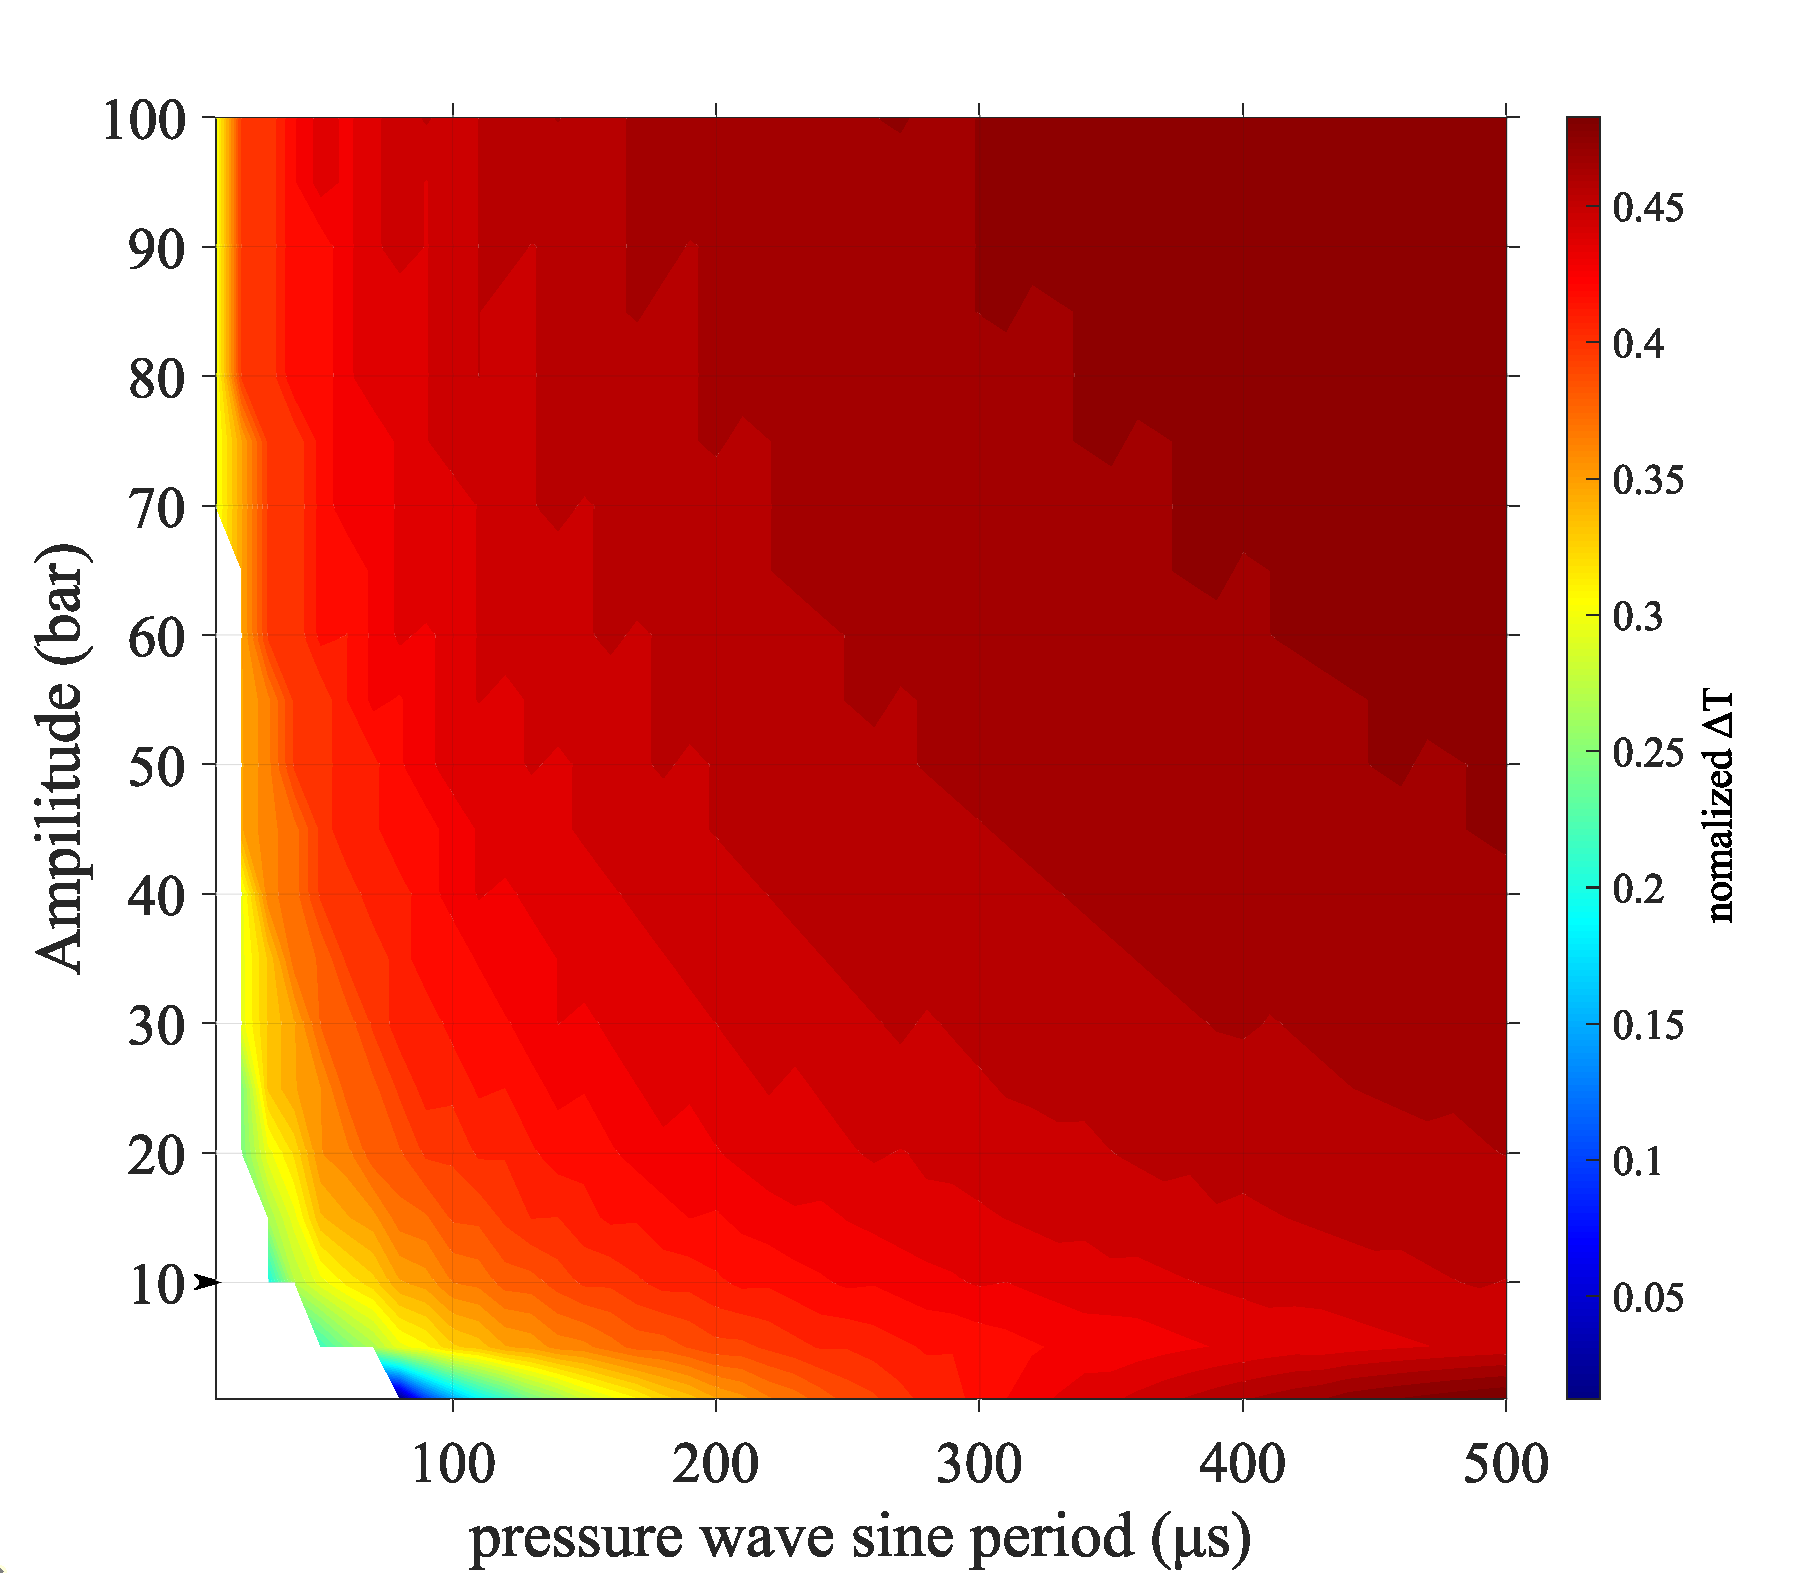
\includegraphics[width=0.6\linewidth]{img/fig5.25-eps-converted-to.pdf}
  \caption{压力波振幅和压力波周期影响下,受迫脉动空泡第一周期自小空泡向大空泡转换的相对时间位置($\Delta T/T_\mathrm{sine}$)云图。
}
  \label{fig:5.25}
\end{figure}

如本章实验所述,其压力波的正压部分压强达到
8bar,负压部分压强可达到-6bar,此取值在线性声压区。考虑线性声压区可以达到几十兆帕,即几百巴,其对空泡脉动可能形成不同效果。本节采用的式
5.2. X 中声压参量从 1bar 到 100bar,以研究空泡受压力波振幅的影响。
通过对比 10bar 与 100bar 的计算结果,上一节中给出的规律同样适用于 100bar
振幅的压力波。但结果中的一些特殊节点表现出随压力波振幅变化的规律。
最主要的,就是空泡溃灭模式转变的节点,也就是由正压强迫溃灭的小空泡到负压拉伸至超量膨胀状态的大空泡的溃灭两种溃灭模式的转变节点。其一般在压力波由正压向负压转换的节点之前,也就是
$T_\mathrm{sine}/2$ 之前。图\ref{fig:5.25} 
中给出了这个转换节点所处的相对相位($\Delta T / T_\mathrm{sine}$)基于压力波周期和振幅的云图。同样的,因为空泡溃灭声波的普遍减弱区一般存在且靠近于这个转换节点前非常近的距离,这里就不对其相对位置进行量化,而只针对小空泡到大空泡的转换进行讨论。
从图中,我们可以看到随着压力波的正弦周期的增长,转换节点的相对相位也呈增长趋势。同样的,
在同压力周期情况下,压力波振幅的增长也伴随这相对相位的增加。这一定程度上代表了高声压对空泡受迫溃灭的加速效果更好,这种加速并不是线性的。压力波振幅越高,空泡的溃灭模式转变的节点越靠近声波相位转变的节点。也就是越高频,声压越低,空泡的脉动和声压的相位延迟越大。




\begin{figure}[H]
  \centering
  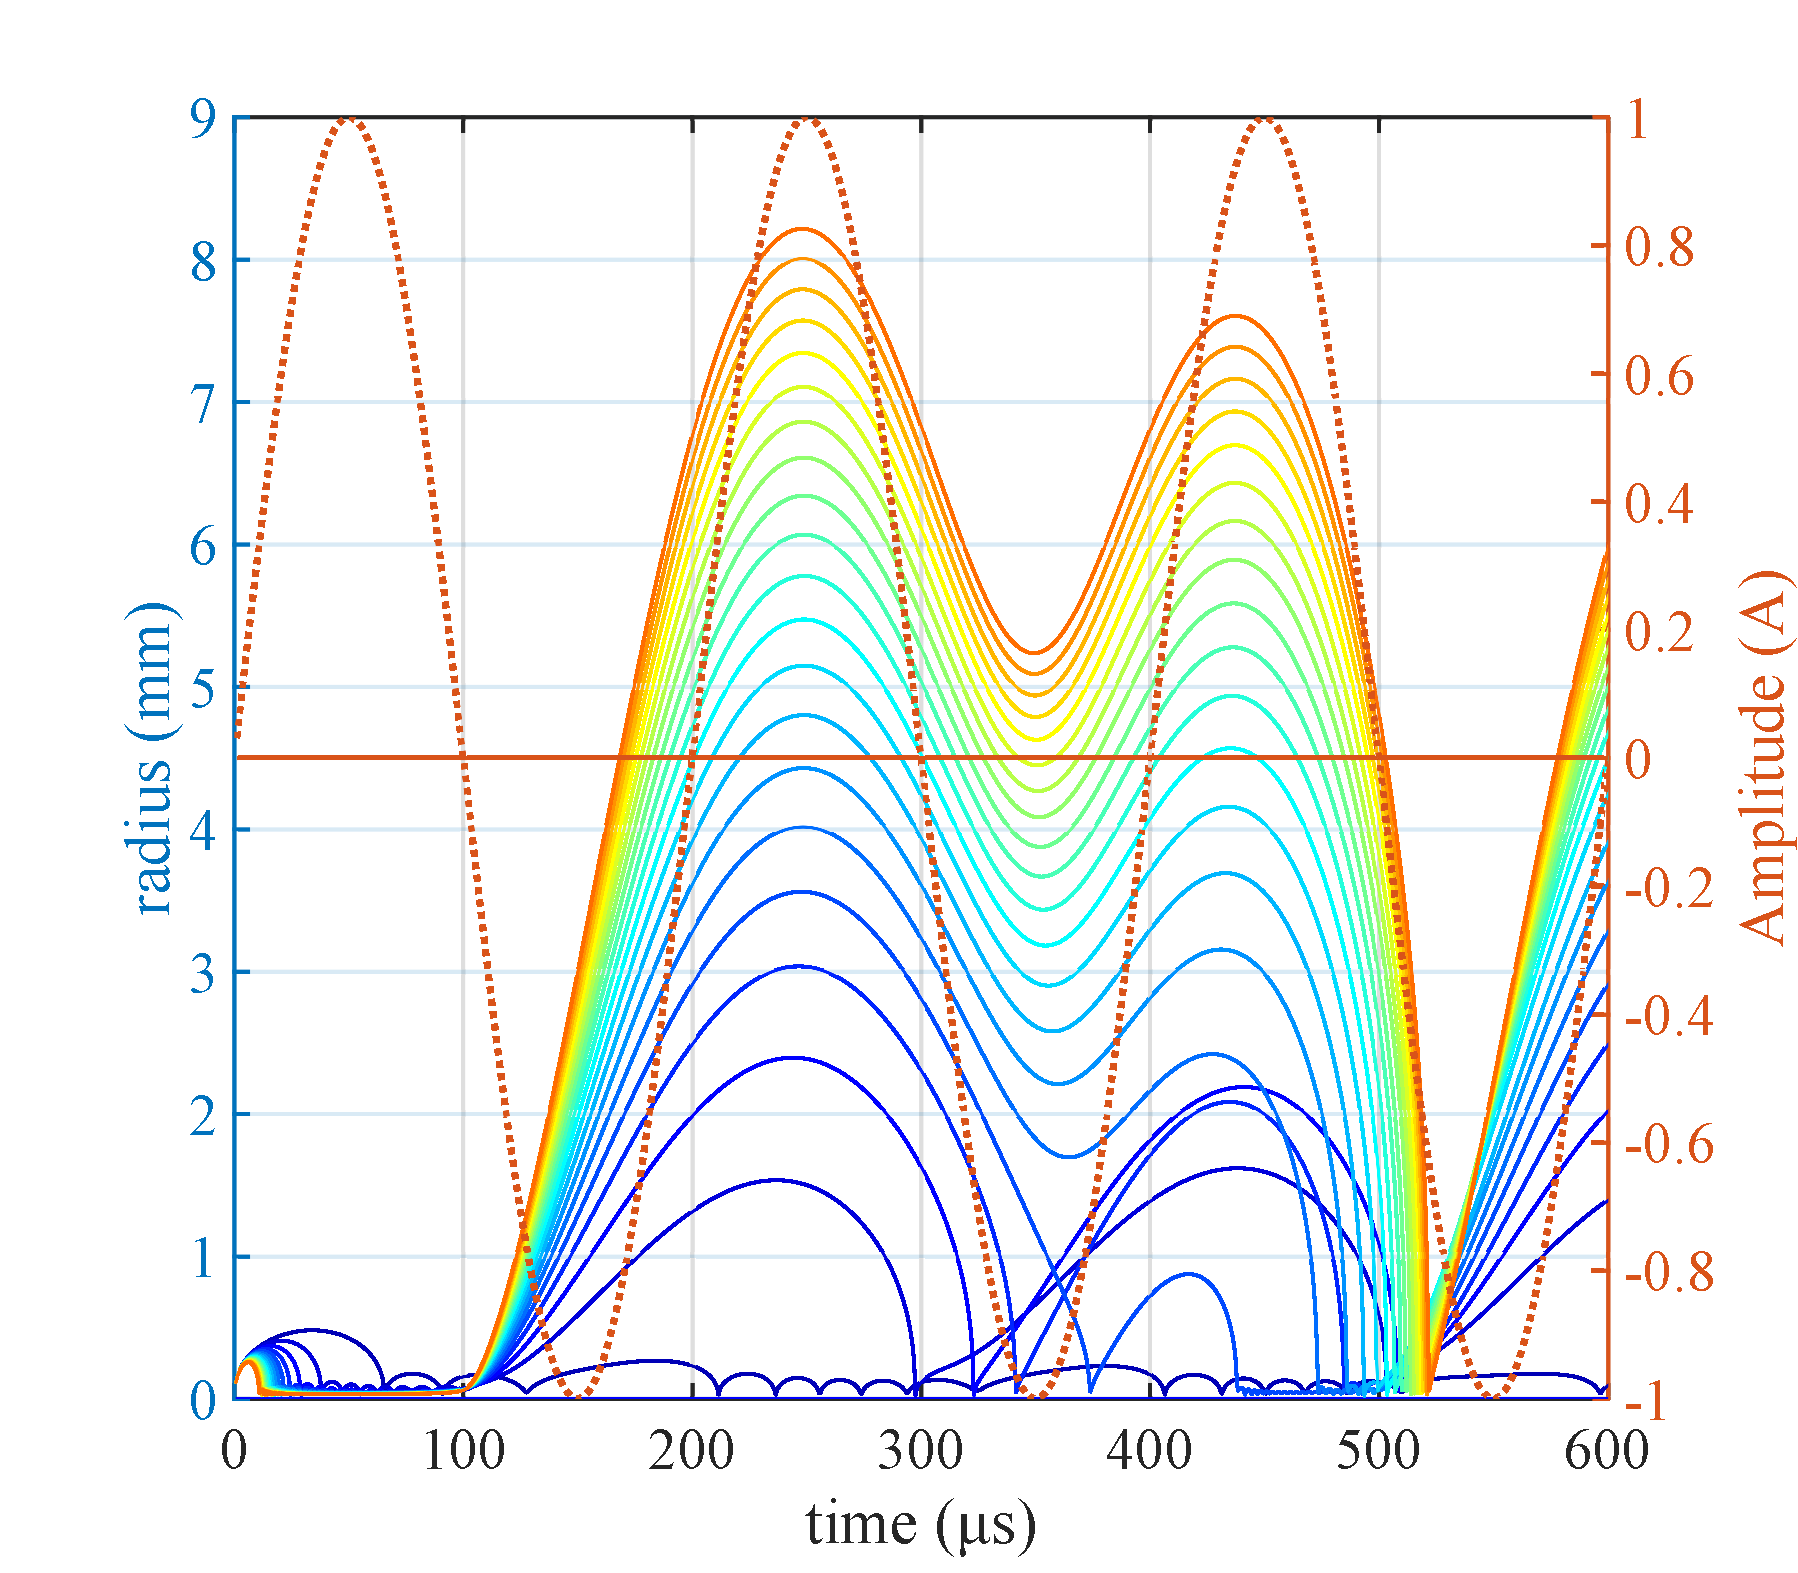
\includegraphics[width=0.7\linewidth]{img/fig5.26-eps-converted-to.pdf}
  \caption[驱动压力波振幅对空泡脉动的影响曲线图]{驱动压力波振幅对空泡脉动的影响曲线图。
$T_\mathrm{sine}=200 \mu s$,$T_\mathrm{posip}=100\mu s$,$\eta =1.0$,$A=(0,\, 1,\,5:5:100)\, \mathrm {bar}$。黑色曲线是无驱动压力波,自蓝至红实线压强逐渐增强。}
  \label{fig:5.26}
\end{figure}

图 \ref{fig:5.26} 
给出了一例驱动压力波振幅对空泡半径影响的曲线。其取自空泡和压力波同时产生的案例,也就是
$\Delta T= 0$ 。图中给出了无压力波影响(黑色曲线),1bar 振幅,和 5:5:
100 bar 二十个不同振幅(自蓝到红,彩虹色标注),共 22
条曲线。从图中可以看到,在第一个脉动周期空泡都产生了受迫溃灭。在第二个膨胀收缩周期内,除了
0bar 和 1bar
两种情况外,其他情况下空泡半径基本与压力波同相位的。也就是声压达到最大时空泡达到最大泡半径。在大振幅也就是高声压情境下,空泡的第二次脉动形成了一种不溃灭而直接回弹膨胀形成一个脉动周期内的第二个半径极值峰。这种不溃灭而直接回弹发生处一般在压力波的波谷处。当简化的用理想气体的波义耳定律理解空泡内压与空泡半径关系时,有
$p_\mathrm{B}\propto R^{-3}$,也就是在正实数的取值范围内,$p_\mathrm{B}$
的增长与 $R$
的减小不是同阶的。就意味着正压对空泡的压缩造成的小空泡溃灭模式中,因驱动声压增长而形成的空泡最大泡半径的减小是不明显的。这就使在正压压制空泡大小后的负压拉伸效果远远高于压缩效果。也就是说在这个案例下,空泡的膨胀基本同起点,但最大值取决与负压相而相差很大。因为负压形成的空泡的超量膨胀,使其在正压相仍有膨胀趋势,并基本与正压同相位,这就使正压在半个正压相时间内对空泡的压缩不足以完全抵消负压形成的效果,从而在接下来的负压相而再次膨胀。同样的因为相位延迟,在下一个负压相内,负压在半个负压相时间内对空泡的膨胀不足以完全抵消正压形成的减速效果,从而形成小峰值,和相位延迟的再次提前。也就以位置,空泡能够在更长的正压相内保持收缩,从而形成溃灭。但也正是由于这种延迟的溃灭,这种一次溃灭可能有多个半径极值峰的现象,造成了空泡的第二次溃灭时间的跳变。

\begin{figure}[H]
  \centering
  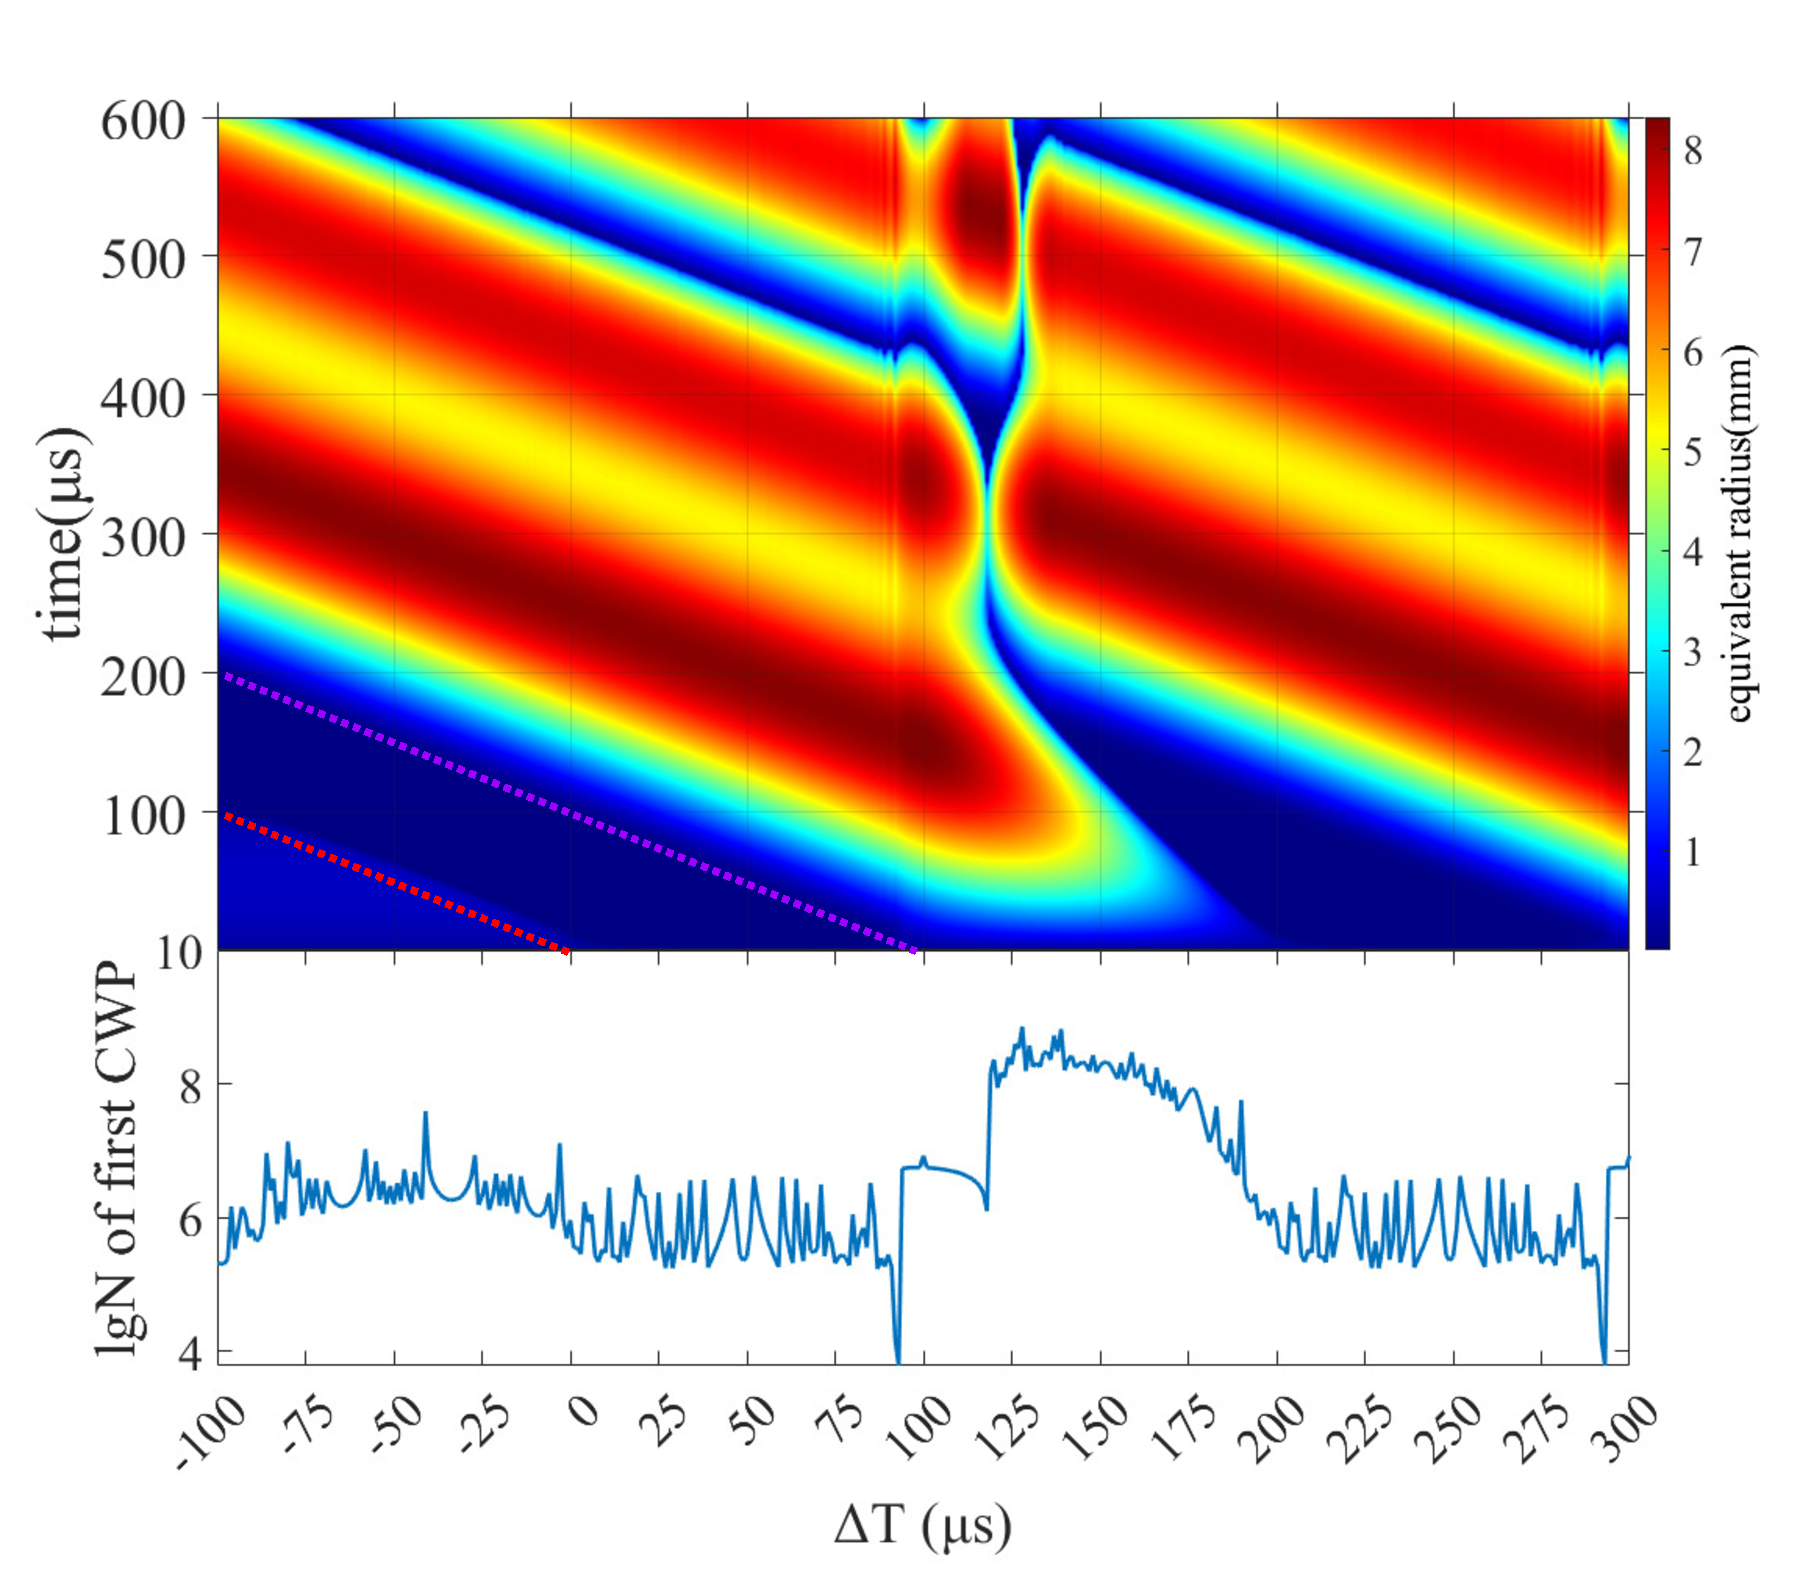
\includegraphics[width=0.9\linewidth]{img/fig5.27-eps-converted-to.pdf}
  \caption[$100\mathrm{bar}$时的正压相与周期相等情况的溃灭波压力对数图]{$100\mathrm{bar}$
振幅下,正弦正压相周期等于空泡第一脉动周期情景的,空泡受迫脉动的半径云图和空泡第一次溃灭产生的溃灭波压强(CWP)的对数级图。对应于
$10\mathrm{bar}$ 振幅下,图 \ref{fig:5.22} 
。$T_\mathrm{sine}=200 \mu s$,$T_\mathrm{posip}=100\mu s$,$\eta =1.0$,$A=100\, \mathrm {bar}$。}
  \label{fig:5.27}
\end{figure}

对比图 \ref{fig:5.27} 和图 \ref{fig:5.22} 
所示,在不同振幅下,随着振幅的增长形成在半径上向低频高周期驱动压结果变化的趋势(图\ref{fig:5.23} 
就是低频和高振幅都会造成空泡最大泡半径的超量膨胀,在空泡寿命上向高频低周期驱动压结果变化的趋势(图
\ref{fig:5.21} )也就是高频和高振幅都会造成空泡单次溃灭多个半径极值峰,越高第二高极值峰越长越高。

\begin{figure}[H]
  \centering
  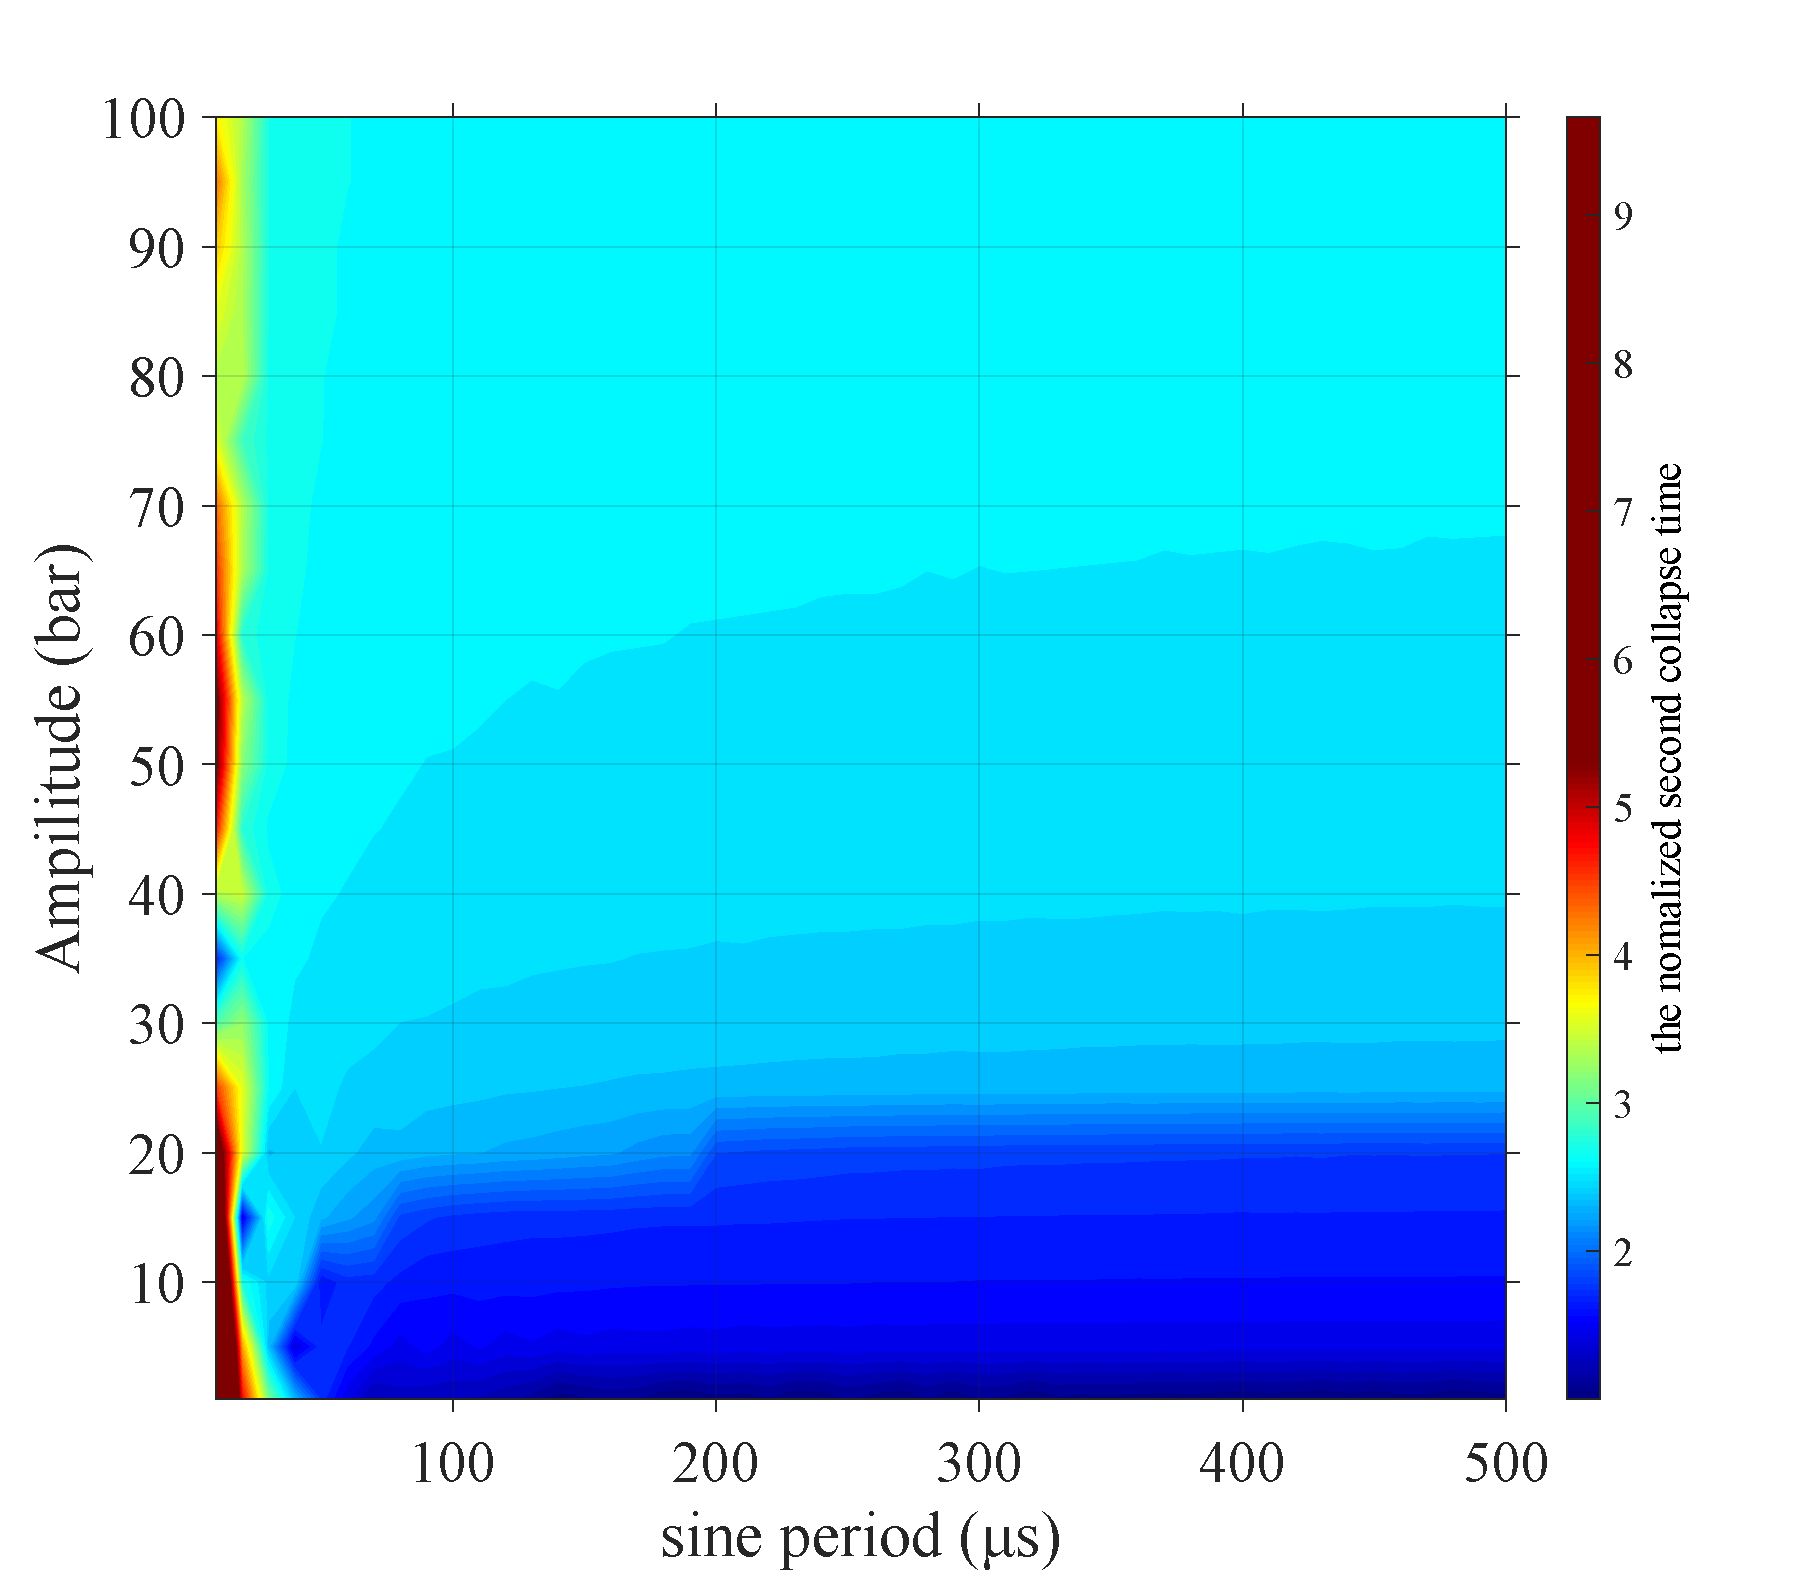
\includegraphics[width=0.7\linewidth]{img/fig5.28.pdf}
  \caption[$\Delta T=0$
时,不同振幅和周期的压力波导致的空泡第二次溃灭时间云图]{$\Delta T=0$
时,不同振幅和周期的压力波导致的空泡第二次溃灭时间云图。压力波振幅导致的其负压相推迟空泡溃灭时间。}
  \label{fig:5.28}
\end{figure}

如图 \ref{fig:5.28} 
给出的第二次溃灭相对时间($t/T_\mathrm{sine}$)所示,压力波振幅越高,其溃灭相对时间越晚。可以预测,随着振幅的继续增高,空泡有可能继续推迟其溃灭时间到形成三个半径极值峰甚至更多。且随着压力波周期的增加,则有溃灭时间减少的趋势,也就是前文所述,高频压力波会强迫空泡形成不溃灭的振动。



\section{本章总结}
本章中,利用自由下落的试管撞击金属平台这样一个简单的实验装置,研究了重力对空泡脉动的影响,以及因撞击产生的压力波和其在自由界面反射形成的舒张波对激光空泡脉动的影响。将实验结果与理想球形空泡受该冲击压力影响的计算结果进行了对比。并展示了决定于空泡产生时间和冲击压力波相位差的空泡动力学。
实验中,空泡的最大泡半径变化区间为 $100\,\mu$ m and $2500\,\mu$
m。当压力波的负压相晚于空泡产生而到达空泡位置,空泡在溃灭后,通常会被舒展波拉扯成一团小空泡团簇,而不是一个大空泡。但压力波的负压相在空泡溃灭前到达空泡,空泡会被拉扯以停止溃灭并回弹或直接膨胀成一个大空泡。而压力波的正压相对空泡的压缩,通常会加强空泡的溃灭,并产生更强的溃灭冲击声压。
而且,单个气泡动力学可以用 Keller-Miksis
模型很好地描述,在某种程度上也可以对空泡团簇簇动力学进行描述,这意味着空泡团簇的行为类似于单个气泡。
这种简单的实验技术即将激光诱导气泡的容器自由落体并撞击产生压力波,可以简单的获得暴露在低频高振幅的压力波下的空泡。该技术可能有利于增强激光诱导空化气泡群的溃灭能量聚焦,以改善早期尝试
\cite{ohl_luminescence_2000,duplat_luminescence_2015}。

同时拓展地,数值研究了正弦压力波对空泡脉动的影响。空泡在零负载状态下脉动时受到正压会加速溃灭并形成辐射声压加强,特别是在最大泡半径附近开始暴露产生最强的声压辐射加强。空泡诞生在正压范围内最大泡半径严重减小,但辐射声压没有明显加强和减弱。空泡诞生在负压相会产生空泡的超量膨胀,并取决于溃灭时压力相位而产生辐射声压的加强和减弱。低频和高振幅都会造成空泡最大泡半径的超量膨胀,高频和高振幅都会造成空泡单次溃灭含多个半径极值峰。

未来可以利用本章的结果以实现在各种工程中实现空泡的溃灭加强和减弱等。